\documentclass[11pt]{article}
\usepackage[margin=2cm]{geometry}
\usepackage{amsmath,amssymb}
\usepackage{graphicx}
\usepackage{booktabs}
\usepackage{array}
\usepackage{xcolor}
\usepackage[breakable]{tcolorbox}
\usepackage{enumitem}
\usepackage[hidelinks]{hyperref}
\allowdisplaybreaks
\setlength{\parindent}{0pt}
\setlength{\parskip}{4pt}
\definecolor{stepc}{HTML}{1F4E9E}
\definecolor{ansc}{HTML}{0B6E4F}
\newcommand{\solstep}[2]{\par\medskip{\color{stepc}\textbf{Step #1 --- #2}}\par\nopagebreak}
\newtcolorbox{probbox}[1]{colback=white,colframe=black!55,fonttitle=\bfseries,title={#1}}
\newtcolorbox{ansbox}{breakable,colback=ansc!6,colframe=ansc,fonttitle=\bfseries,title={Answer}}
\newtcolorbox{cardbox}[1]{breakable,colback=stepc!4,colframe=stepc,fonttitle=\bfseries,title={#1}}
\graphicspath{{../../../output/lecture1/1B_superposition/}}
\title{Set 1B: DC + AC Superposition}
\author{ECEN 325 --- Lecture 1 (Linear Network Analysis) practice set}
\date{}
\begin{document}
\maketitle

\textbf{What this set trains.} Circuits with DC supplies \emph{and} an AC input. You split the problem in two
(superposition): a DC circuit that gives $V_{o,dc}$ (capacitors open, inductors shorted) and an AC circuit that
gives $H(s)$ and $v_{o,ac}(t)$ (supplies grounded). The DC part uses only one tool, the divider between two
voltages. Problems 1--6 are easy, 7--12 medium, 13--18 hard. Try each problem before looking at its solution.


\begin{cardbox}{The Lecture-1 pipeline (use it for every problem in this set)}
\textbf{Tools --- this is all the theory you need:}
\begin{enumerate}[label=\textbf{T\arabic*},leftmargin=2.2em,itemsep=1pt]
\item \emph{Impedances:} $Z_R=R$, $Z_C=\frac{1}{sC}$, $Z_L=sL$. Series: add. Parallel:
      $Z_a\parallel Z_b=\frac{Z_aZ_b}{Z_a+Z_b}$.
\item \emph{Voltage divider:} if $Z_{top}$ connects $V_{in}$ to a node and $Z_{bot}$ is everything from that
      node to ground, then $V_{node}=V_{in}\,\frac{Z_{bot}}{Z_{top}+Z_{bot}}$.
\item \emph{Divider between two voltages (DC):} a node tied to $V_a$ through $R_a$ and to $V_b$ through $R_b$ sits at
      $V=V_b+(V_a-V_b)\frac{R_b}{R_a+R_b}$, and looks like a source $V$ with resistance $R_a\parallel R_b$
      (its Thevenin pair).
\item \emph{Dependent sources:} a VCVS forces $V=kV_x$; a VCCS drives the current $gV_x$ through the impedance $Z$
      hanging on its node, so $V=\pm gV_x Z$ (sign from the arrow).
\item \emph{Sinusoids:} $A\sin(\omega t+\theta)\ \to\ |H(j\omega)|\,A\sin\big(\omega t+\theta+\angle H(j\omega)\big)$.
\item \emph{Bode rules:} a pole at $p$ bends the magnitude by $-20$\,dB/dec above $p$, a zero by $+20$\,dB/dec;
      $\frac{1}{1+s/p}$ is $0$\,dB below $p$; $\frac{s}{s+p}$ is $0$\,dB above $p$.
\end{enumerate}
\textbf{Steps:}
\begin{enumerate}[leftmargin=2.2em,itemsep=1pt]
\item \emph{Sources.} DC and AC both present $\Rightarrow$ superposition $V_o=V_{o,dc}+v_{o,ac}$.
\item \emph{DC circuit:} $V_i\to0$, $C\to$ open, $L\to$ short; reduce toward $V_o$ with T3.
\item \emph{AC circuit:} DC supplies $\to 0$ (rails become ground); merge parallel resistors.
\item \emph{Divider chain:} name the nodes from $V_i$ to $V_o$; $H=\prod$ (node-to-node ratios), each by T2 or T4,
      using the impedance seen looking right from each node.
\item \emph{Standard form:} simplify, find the roots, write $H=K\cdot\prod(\text{factors})$.
\item \emph{Bode:} start from the low-frequency slope, bend by $\pm20$\,dB/dec at each corner.
\item \emph{Output:} evaluate each factor at $s=j\omega_{in}$, multiply magnitudes, add angles, apply T5 and add $V_{o,dc}$.
\end{enumerate}
\end{cardbox}

\section*{Problems}
\subsection*{Easy problems}
\begin{probbox}{Problem 1B.1 \hfill Easy}
For the circuit below: (a) find the AC transfer function $H(s)=\dfrac{V_o(s)}{V_i(s)}$ and sketch its magnitude Bode plot; (b) find the steady-state output $V_o(t)$ for $V_i(t) = 0.5\sin\left(2\pi\cdot 100\,t\right)$.
\begin{center}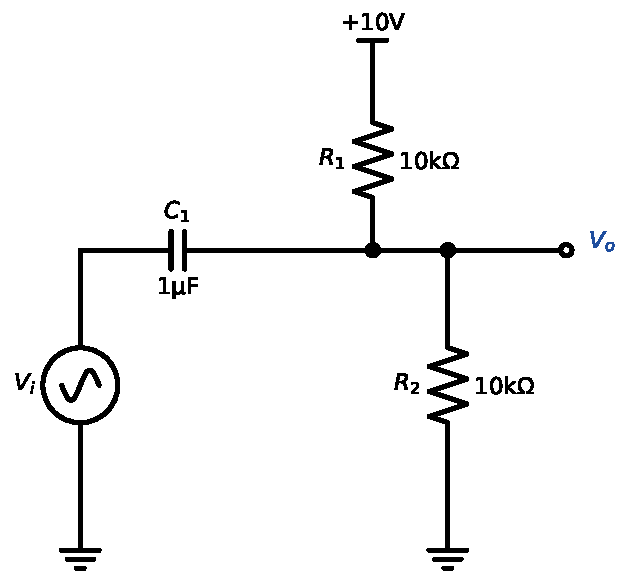
\includegraphics[width=0.8\linewidth,height=5.5cm,keepaspectratio]{p01_circuit}\end{center}
\end{probbox}

\begin{probbox}{Problem 1B.2 \hfill Easy}
For the circuit below: (a) find the AC transfer function $H(s)=\dfrac{V_o(s)}{V_i(s)}$ and sketch its magnitude Bode plot; (b) find the steady-state output $V_o(t)$ for $V_i(t) = 1\sin\left(2\pi\cdot 50\,t\right)$.
\begin{center}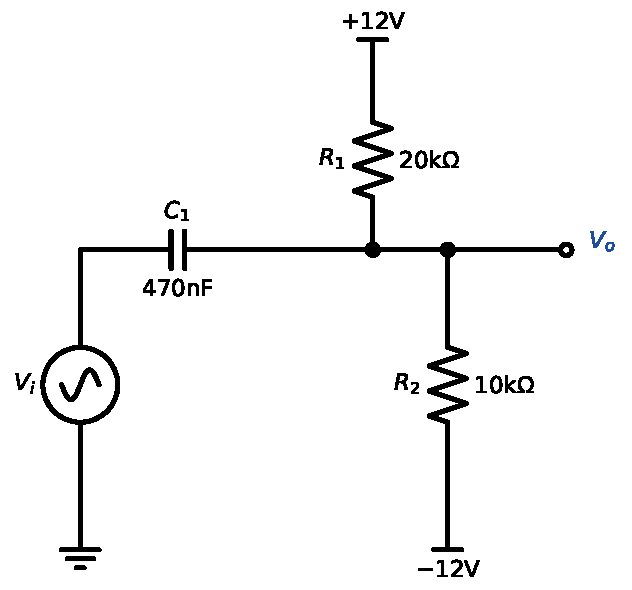
\includegraphics[width=0.8\linewidth,height=5.5cm,keepaspectratio]{p02_circuit}\end{center}
\end{probbox}

\begin{probbox}{Problem 1B.3 \hfill Easy}
For the circuit below: (a) find the AC transfer function $H(s)=\dfrac{V_o(s)}{V_i(s)}$ and sketch its magnitude Bode plot; (b) find the steady-state output $V_o(t)$ for $V_i(t) = 0.5\sin\left(2\pi\cdot 1000\,t\right)$.
\begin{center}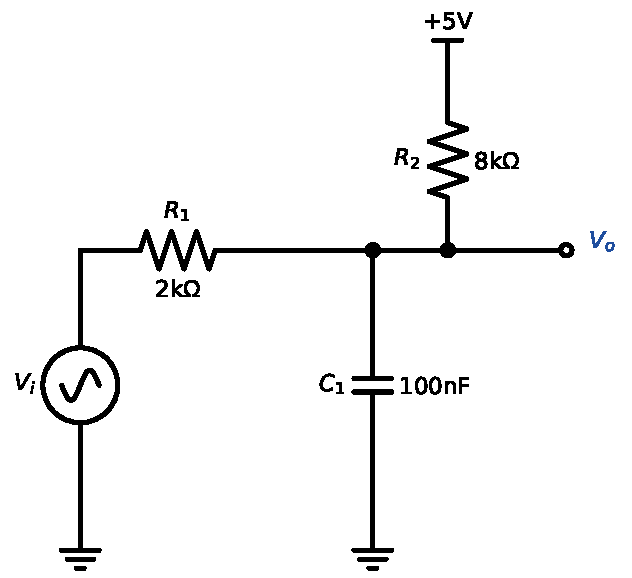
\includegraphics[width=0.8\linewidth,height=5.5cm,keepaspectratio]{p03_circuit}\end{center}
\end{probbox}

\begin{probbox}{Problem 1B.4 \hfill Easy}
For the circuit below: (a) find the AC transfer function $H(s)=\dfrac{V_o(s)}{V_i(s)}$ and sketch its magnitude Bode plot; (b) find the steady-state output $V_o(t)$ for $V_i(t) = 0.2\sin\left(2\pi\cdot 100\,t\right)$.
\begin{center}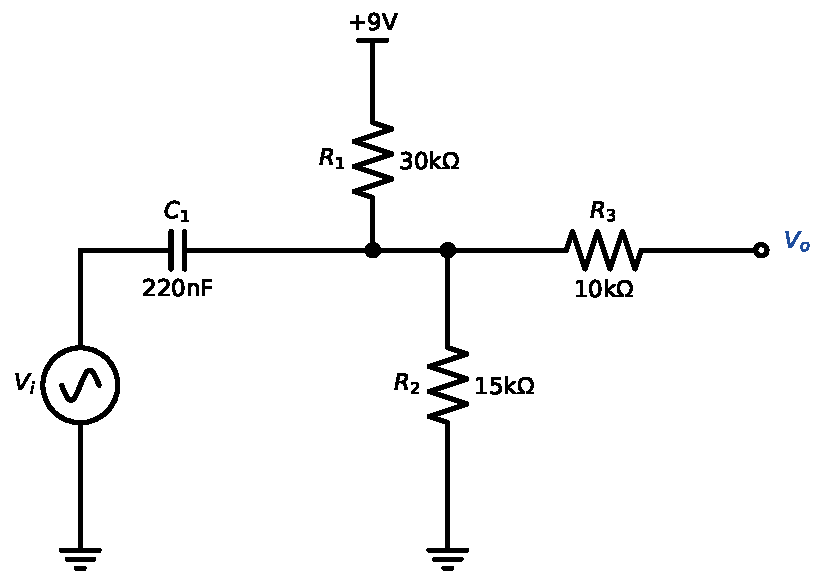
\includegraphics[width=0.8\linewidth,height=5.5cm,keepaspectratio]{p04_circuit}\end{center}
\end{probbox}

\begin{probbox}{Problem 1B.5 \hfill Easy}
For the circuit below: (a) find the AC transfer function $H(s)=\dfrac{V_o(s)}{V_i(s)}$ and sketch its magnitude Bode plot; (b) find the steady-state output $V_o(t)$ for $V_i(t) = 1\sin\left(2\pi\cdot 500\,t\right)$.
\begin{center}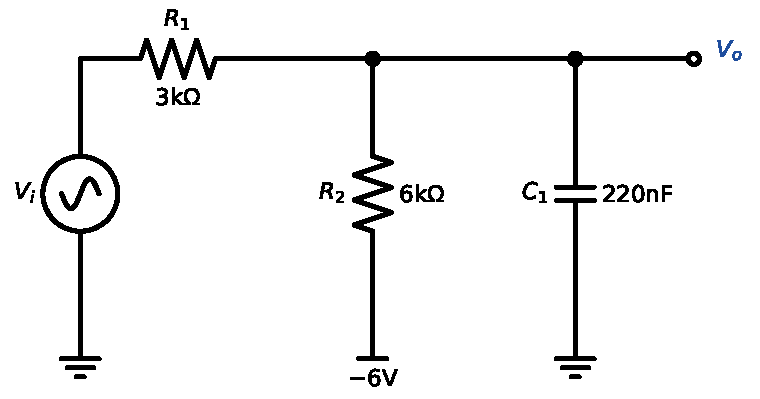
\includegraphics[width=0.8\linewidth,height=5.5cm,keepaspectratio]{p05_circuit}\end{center}
\end{probbox}

\begin{probbox}{Problem 1B.6 \hfill Easy}
For the circuit below: (a) find the AC transfer function $H(s)=\dfrac{V_o(s)}{V_i(s)}$ and sketch its magnitude Bode plot; (b) find the steady-state output $V_o(t)$ for $V_i(t) = 0.3\sin\left(2\pi\cdot 20\,t\right)$.
\begin{center}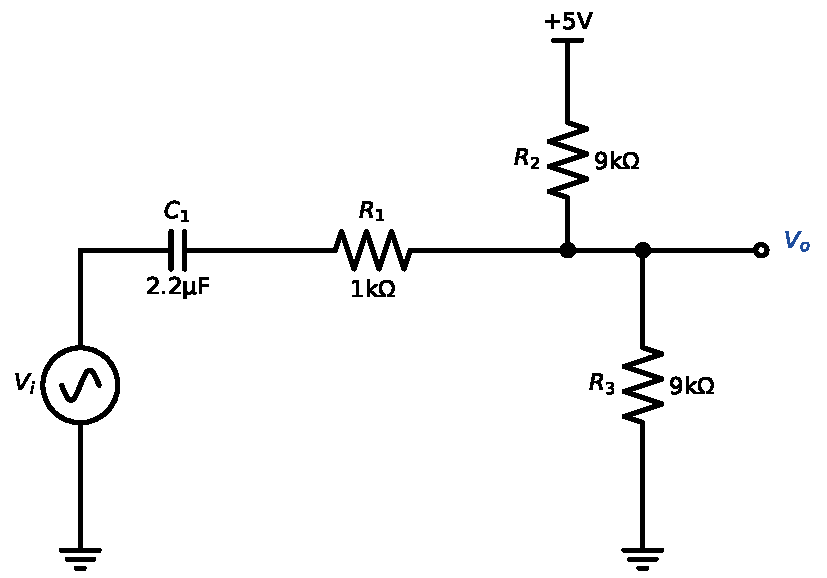
\includegraphics[width=0.8\linewidth,height=5.5cm,keepaspectratio]{p06_circuit}\end{center}
\end{probbox}

\subsection*{Medium problems}
\begin{probbox}{Problem 1B.7 \hfill Medium}
For the circuit below: (a) find the AC transfer function $H(s)=\dfrac{V_o(s)}{V_i(s)}$ and sketch its magnitude Bode plot; (b) find the steady-state output $V_o(t)$ for $V_i(t) = 0.5\sin\left(2\pi\cdot 1000\,t\right)$.
\begin{center}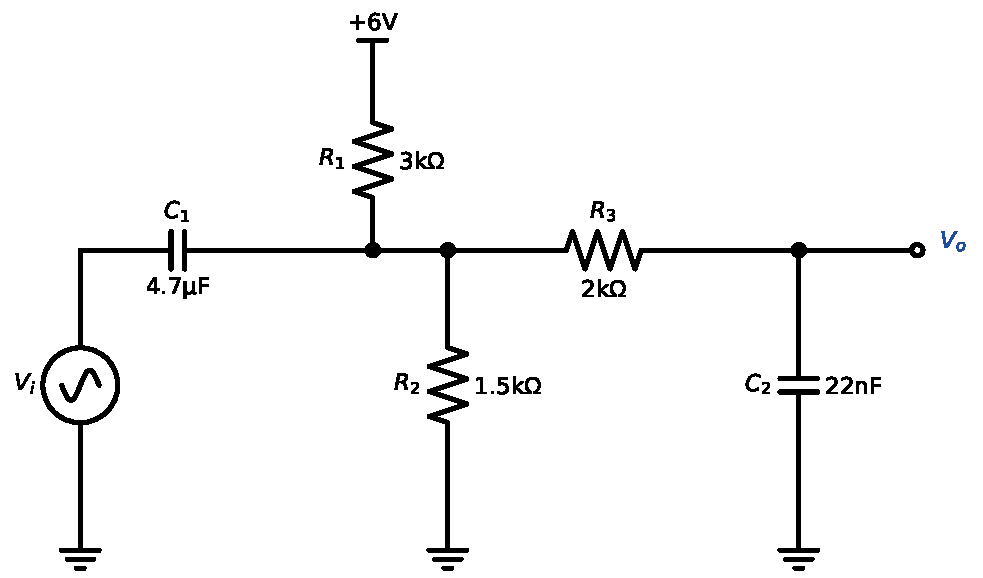
\includegraphics[width=0.8\linewidth,height=5.5cm,keepaspectratio]{p07_circuit}\end{center}
\end{probbox}

\begin{probbox}{Problem 1B.8 \hfill Medium}
For the circuit below: (a) find the AC transfer function $H(s)=\dfrac{V_o(s)}{V_i(s)}$ and sketch its magnitude Bode plot; (b) find the steady-state output $V_o(t)$ for $V_i(t) = 0.5\sin\left(2\pi\cdot 2000\,t\right)$.
\begin{center}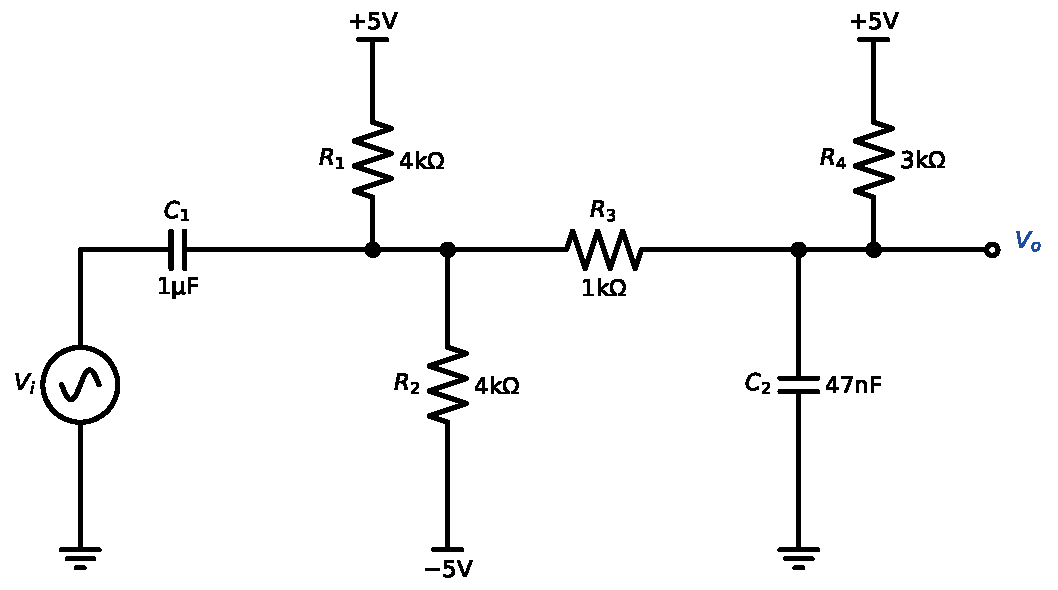
\includegraphics[width=0.8\linewidth,height=5.5cm,keepaspectratio]{p08_circuit}\end{center}
\end{probbox}

\begin{probbox}{Problem 1B.9 \hfill Medium}
For the circuit below: (a) find the AC transfer function $H(s)=\dfrac{V_o(s)}{V_i(s)}$ and sketch its magnitude Bode plot; (b) find the steady-state output $V_o(t)$ for $V_i(t) = 1\sin\left(2\pi\cdot 500\,t\right)$.
\begin{center}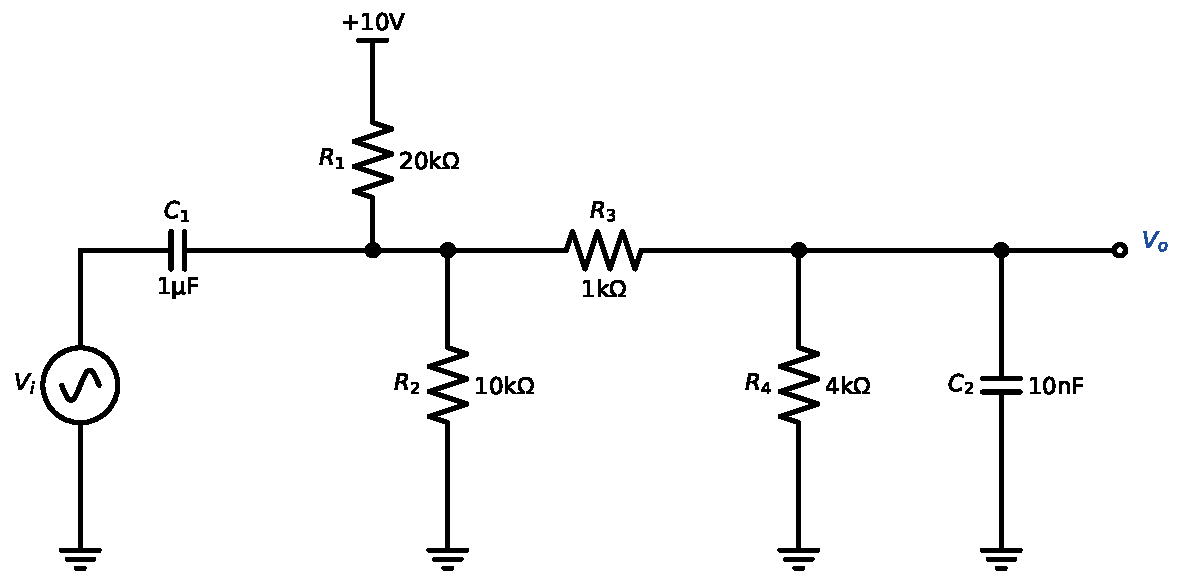
\includegraphics[width=0.8\linewidth,height=5.5cm,keepaspectratio]{p09_circuit}\end{center}
\end{probbox}

\begin{probbox}{Problem 1B.10 \hfill Medium}
For the circuit below: (a) find the AC transfer function $H(s)=\dfrac{V_o(s)}{V_i(s)}$ and sketch its magnitude Bode plot; (b) find the steady-state output $V_o(t)$ for $V_i(t) = 1\sin\left(2\pi\cdot 200\,t\right)$.
\begin{center}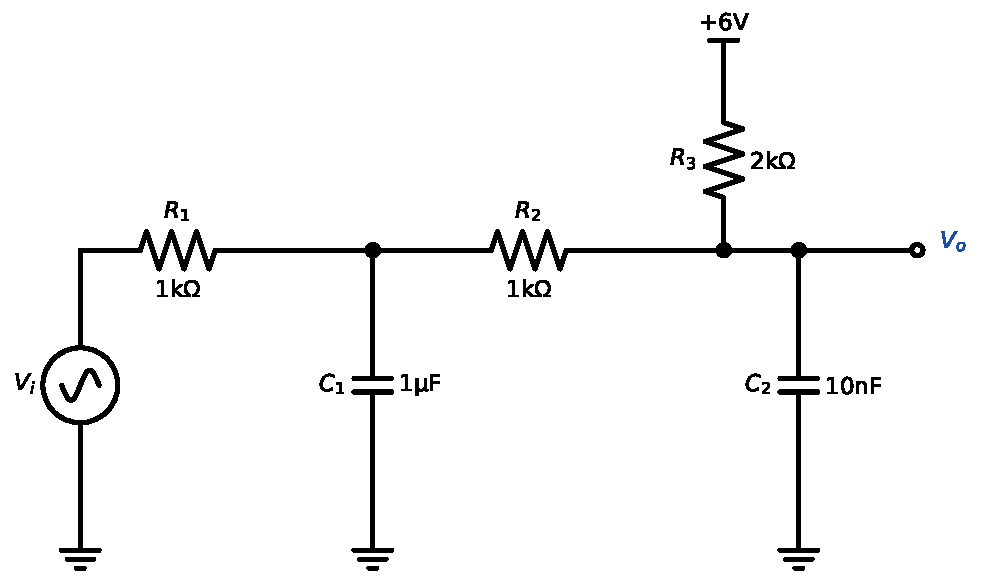
\includegraphics[width=0.8\linewidth,height=5.5cm,keepaspectratio]{p10_circuit}\end{center}
\end{probbox}

\begin{probbox}{Problem 1B.11 \hfill Medium}
For the circuit below: (a) find the AC transfer function $H(s)=\dfrac{V_o(s)}{V_i(s)}$ and sketch its magnitude Bode plot; (b) find the steady-state output $V_o(t)$ for $V_i(t) = 2\sin\left(2\pi\cdot 1000\,t\right)$.
\begin{center}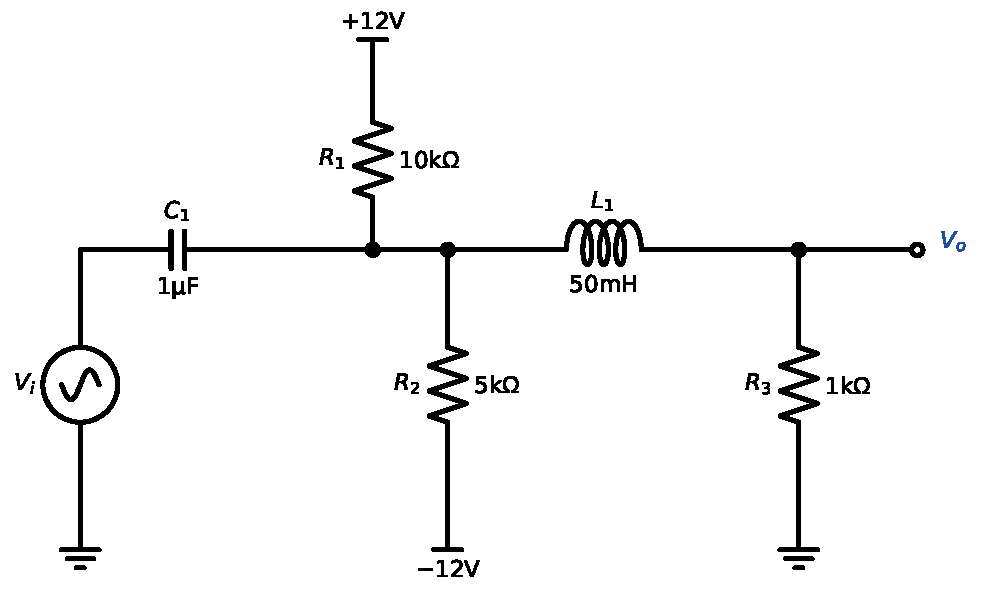
\includegraphics[width=0.8\linewidth,height=5.5cm,keepaspectratio]{p11_circuit}\end{center}
\end{probbox}

\begin{probbox}{Problem 1B.12 \hfill Medium}
For the circuit below: (a) find the AC transfer function $H(s)=\dfrac{V_o(s)}{V_i(s)}$ and sketch its magnitude Bode plot; (b) find the steady-state output $V_o(t)$ for $V_i(t) = 0.4\sin\left(2\pi\cdot 300\,t\right)$.
\begin{center}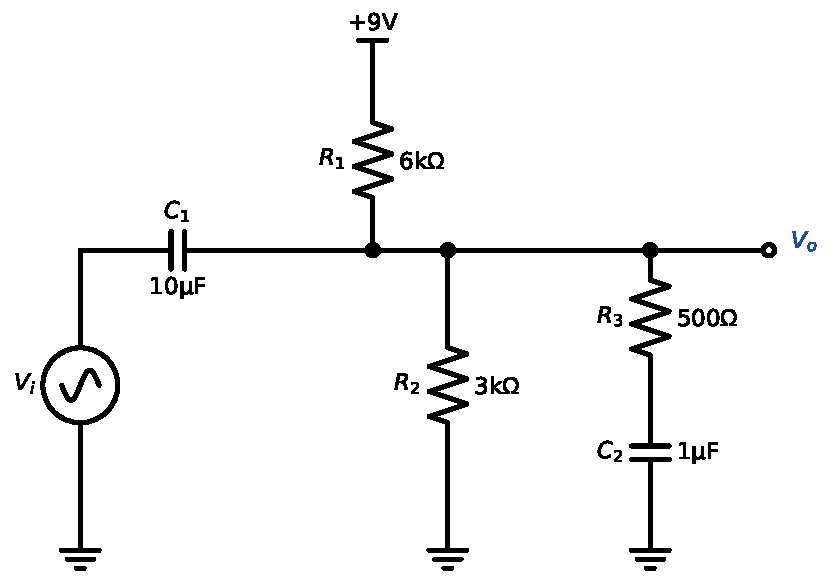
\includegraphics[width=0.8\linewidth,height=5.5cm,keepaspectratio]{p12_circuit}\end{center}
\end{probbox}

\subsection*{Hard problems}
\begin{probbox}{Problem 1B.13 \hfill Hard}
For the circuit below: (a) find the AC transfer function $H(s)=\dfrac{V_o(s)}{V_i(s)}$ and sketch its magnitude Bode plot; (b) find the steady-state output $V_o(t)$ for $V_i(t) = 1.5\sin\left(2\pi\cdot 1000\,t+\frac{\pi}{4}\right)$.
\begin{center}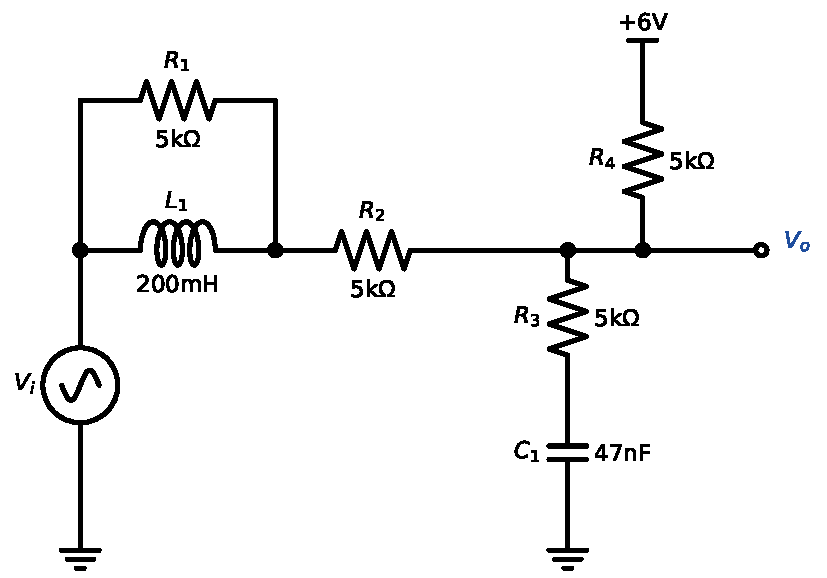
\includegraphics[width=0.8\linewidth,height=5.5cm,keepaspectratio]{p13_circuit}\end{center}
\end{probbox}

\begin{probbox}{Problem 1B.14 \hfill Hard}
For the circuit below: (a) find the AC transfer function $H(s)=\dfrac{V_o(s)}{V_i(s)}$ and sketch its magnitude Bode plot; (b) find the steady-state output $V_o(t)$ for $V_i(t) = 0.5\sin\left(2\pi\cdot 300\,t\right)$. Note that $V_o$ is \emph{not} at the right end: the branch to its right loads it, both at DC and at AC.
\begin{center}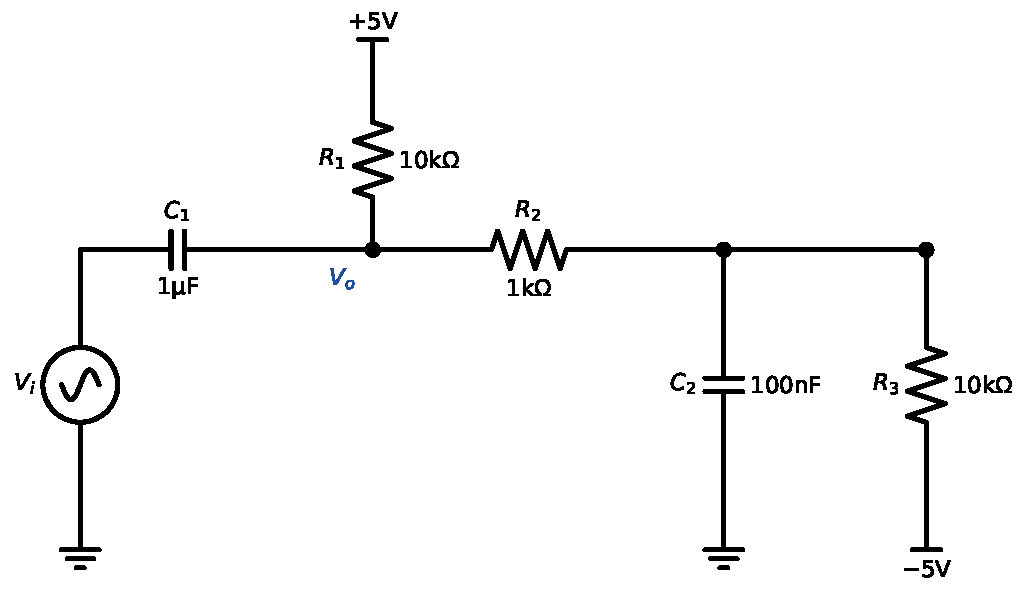
\includegraphics[width=0.8\linewidth,height=5.5cm,keepaspectratio]{p14_circuit}\end{center}
\end{probbox}

\begin{probbox}{Problem 1B.15 \hfill Hard}
For the circuit below: (a) find the AC transfer function $H(s)=\dfrac{V_o(s)}{V_i(s)}$ and sketch its magnitude Bode plot; (b) find the steady-state output $V_o(t)$ for $V_i(t) = 0.3\sin\left(2\pi\cdot 100\,t\right)$.
\begin{center}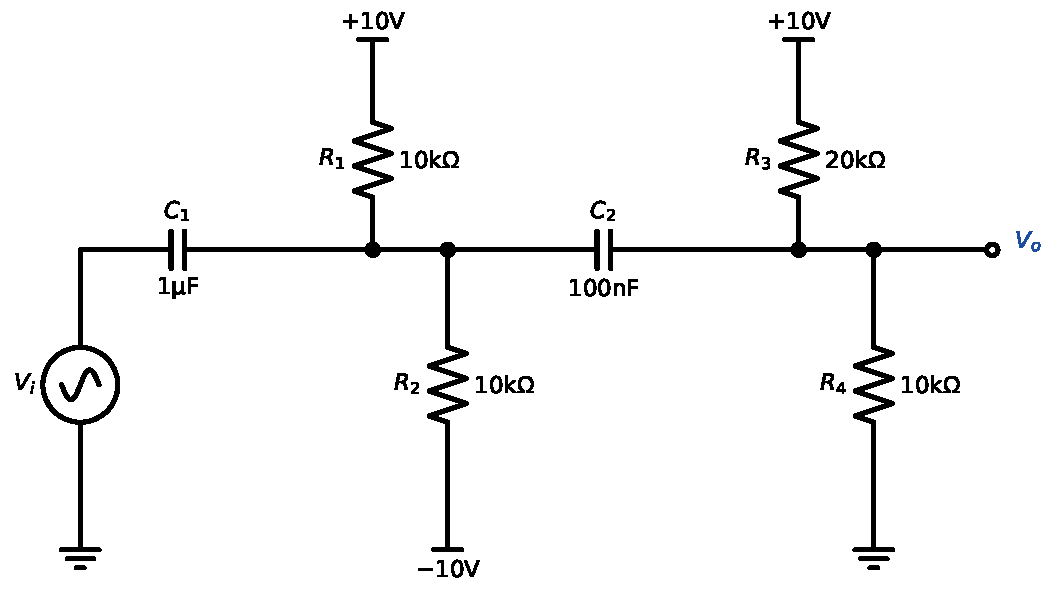
\includegraphics[width=0.8\linewidth,height=5.5cm,keepaspectratio]{p15_circuit}\end{center}
\end{probbox}

\begin{probbox}{Problem 1B.16 \hfill Hard}
For the circuit below: (a) find the AC transfer function $H(s)=\dfrac{V_o(s)}{V_i(s)}$ and sketch its magnitude Bode plot; (b) find the steady-state output $V_o(t)$ for $V_i(t) = 1\cos\left(2\pi\cdot 1000\,t\right)$.
\begin{center}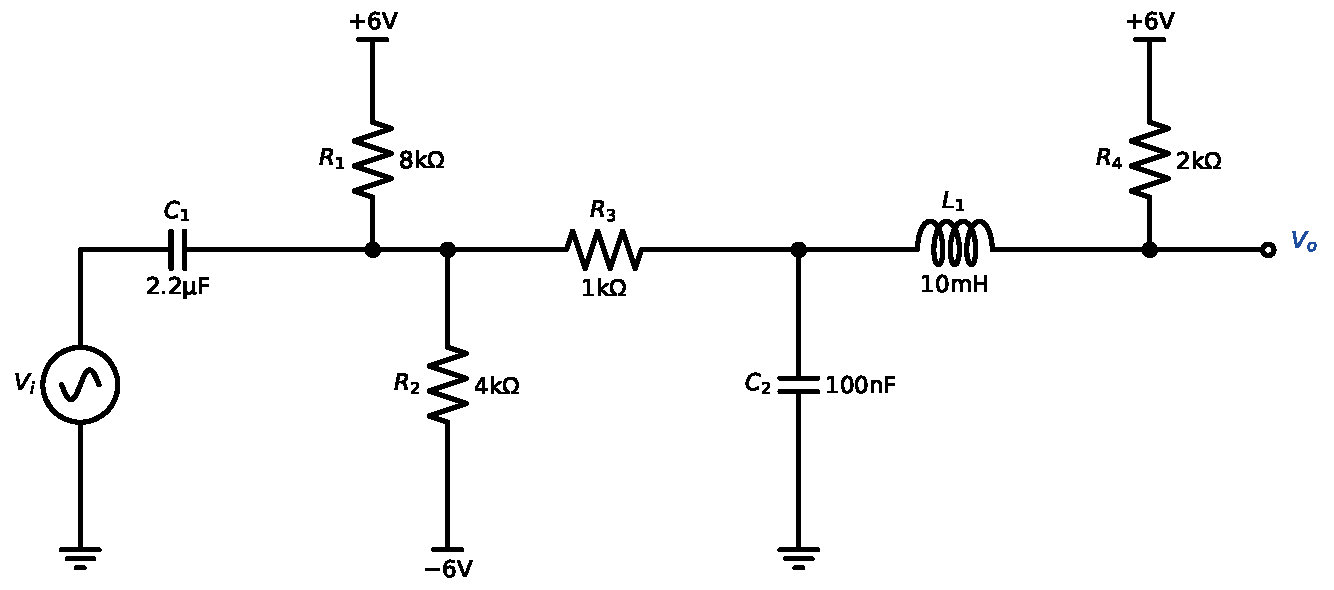
\includegraphics[width=0.8\linewidth,height=5.5cm,keepaspectratio]{p16_circuit}\end{center}
\end{probbox}

\begin{probbox}{Problem 1B.17 \hfill Hard}
For the circuit below: (a) find the AC transfer function $H(s)=\dfrac{V_o(s)}{V_i(s)}$ and sketch its magnitude Bode plot; (b) find the steady-state output $V_o(t)$ for $V_i(t) = 1\cos\left(2\pi\cdot 500\,t-\frac{\pi}{3}\right)$.
\begin{center}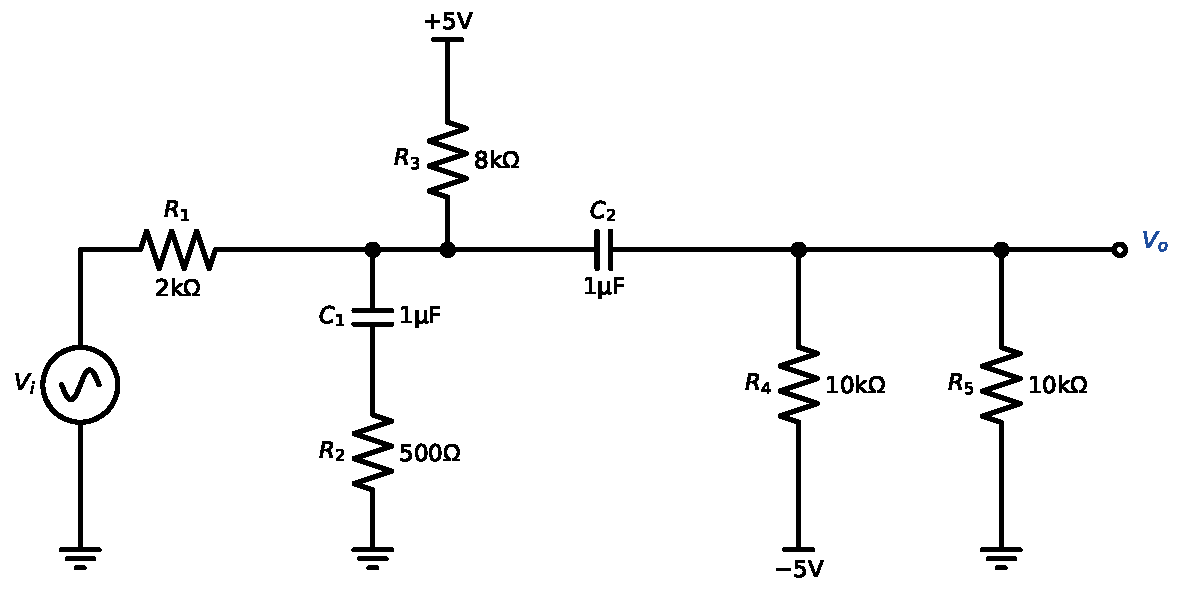
\includegraphics[width=0.8\linewidth,height=5.5cm,keepaspectratio]{p17_circuit}\end{center}
\end{probbox}

\begin{probbox}{Problem 1B.18 \hfill Hard}
For the circuit below: (a) find the AC transfer function $H(s)=\dfrac{V_o(s)}{V_i(s)}$ and sketch its magnitude Bode plot; (b) find the steady-state output $V_o(t)$ for $V_i(t) = 0.5\sin\left(2\pi\cdot 2000\,t+\frac{\pi}{6}\right)$.
\begin{center}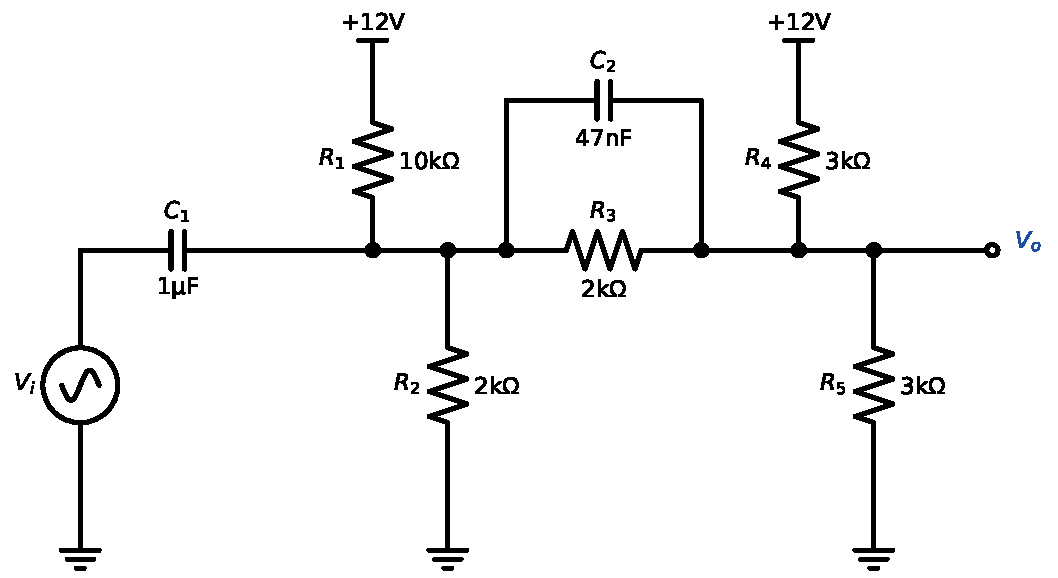
\includegraphics[width=0.8\linewidth,height=5.5cm,keepaspectratio]{p18_circuit}\end{center}
\end{probbox}

\newpage
\section*{Solutions}
Every solution follows the same seven steps of the pipeline card.
\newpage
\subsection*{Solution 1B.1 \hfill Easy}
\begin{center}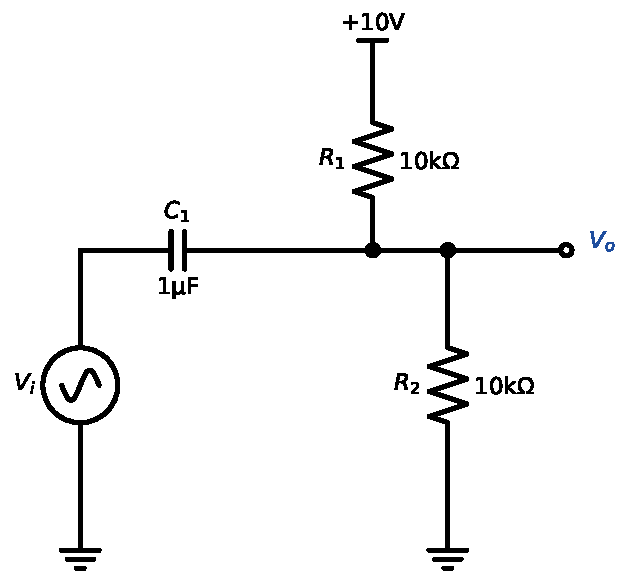
\includegraphics[width=0.8\linewidth,height=4.5cm,keepaspectratio]{p01_circuit}\end{center}
\solstep{1}{Identify the sources}Independent sources: the AC input $V_i(t)$ and the DC supplies $+10\,\mathrm{V}$. Because there are both DC and AC sources, use superposition: $V_o(t) = V_{o,dc} + v_{o,ac}(t)$. Solve the DC circuit (Step 2) and the AC circuit (Steps 3--7) separately, then add.
\solstep{2}{DC circuit $\Rightarrow V_{o,dc}$}DC rules: the AC input is set to zero ($V_i=0$: a wire to ground); every capacitor is an open circuit ($C_{1}$). Only the part of the circuit that is still connected to $V_o$ matters:
\begin{center}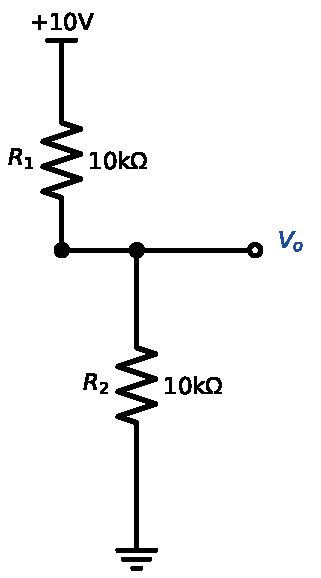
\includegraphics[width=0.55\linewidth,height=5cm,keepaspectratio]{p01_dc}\end{center}

Reduce the circuit with one tool only --- the \emph{divider between two voltages} (tool T3) --- walking toward $V_o$ and keeping a Thevenin pair $(V_{th},R_{th})$ for everything already visited.
\begin{enumerate}[leftmargin=*,itemsep=2pt]
\item Start at the input node: since $V_i=0$ it is tied to ground, i.e. it is an ideal $0\,\mathrm{V}$ source: $(V_{th},R_{th})=(0\,\mathrm{V},\,0\,\Omega)$.
\item $C_{1}$ is a capacitor $\Rightarrow$ open at DC. No DC current can cross it, so everything on its left is disconnected: start fresh after it.
\item Finally, collect everything at the output node $V_o$.
\item First DC path here: $R_{1}$ to the $+10\,\mathrm{V}$ supply, so $(V_{th},R_{th}) = (10\,\mathrm{V},\ 10\,\mathrm{k}\Omega)$.
\item Add $R_{2}$ to ground. Divider between $V_a=10\,\mathrm{V}$ (through $R_a=10\,\mathrm{k}\Omega$) and $V_b=0\,\mathrm{V}$ (through $R_b=10\,\mathrm{k}\Omega$):\[
V_{th} = V_b + (V_a-V_b)\frac{R_b}{R_a+R_b} = 0 + \left(10 - (0)\right)\frac{10\,\mathrm{k}}{10\,\mathrm{k} + 10\,\mathrm{k}} = 5\,\mathrm{V},\qquad R_{th} = R_a\parallel R_b = 5\,\mathrm{k}\Omega
\]

\end{enumerate}

\[
\boxed{V_{o,dc} = 5\,\mathrm{V}}
\]

\solstep{3}{AC circuit}Set every DC supply to zero: each supply rail becomes AC ground. Replace every capacitor by $\frac{1}{sC}$ and every inductor by $sL$.
\begin{itemize}[leftmargin=*,itemsep=2pt]
\item $R_{1}$, $R_{2}$ both go from the same node to (AC) ground, so they are in parallel: $R_{12} = R_{1} \parallel R_{2} = 10\,\mathrm{k} \parallel 10\,\mathrm{k} = 5\,\mathrm{k}\Omega$.
\end{itemize}

AC equivalent circuit (nodes named for the next step):
\begin{center}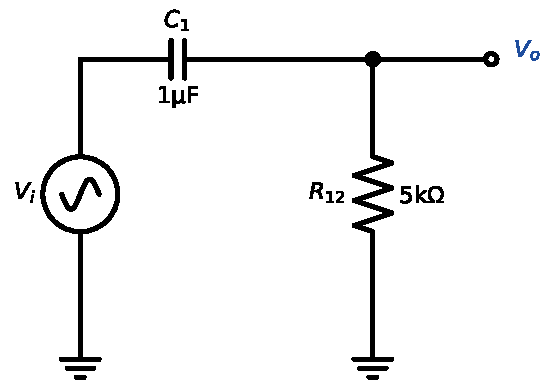
\includegraphics[width=0.95\linewidth,height=5.2cm,keepaspectratio]{p01_ac}\end{center}

\solstep{4}{Transfer function by a chain of dividers}Walk from the input to the output through the named nodes: $V_{i} \to V_{o}$. There is a single link, so $H(s)$ is just one voltage divider (tool T2).
Now each link. {\small (Algebra tip: to simplify a fraction that contains fractions, multiply its top and bottom by every inner denominator; then divide top and bottom by the leading coefficient of the denominator so that it starts with a plain $s^n$.)}
\begin{align*}
\frac{V_{o}}{V_{i}} &= \frac{R_{12}}{\frac{1}{sC_{1}} + R_{12}} = \dfrac{s}{s + 200}
\end{align*}

So:\[
H(s) = \dfrac{s}{s + 200}
\]

\solstep{5}{Standard (Bode-ready) form}Find the roots. Every root $s=-p$ of the denominator is a \emph{pole}, every root $s=-z$ of the numerator is a \emph{zero}; $|p|$ and $|z|$ are the corner frequencies (rad/s).
\begin{itemize}[leftmargin=*,itemsep=2pt]
\item Numerator: it has the factor $s$ $\Rightarrow$ 1 zero at $s=0$.
\item Denominator: $s + 200$; $s + 200 = 0 \Rightarrow s = -200$.
\end{itemize}

Factored form (leading coefficient in front):
\[
H(s) = 1\,\dfrac{s}{(s+200)}
\]

Bode-ready form: rewrite every $(s+p) = p\left(1+\frac{s}{p}\right)$ and $(s+z) = z\left(1+\frac{s}{z}\right)$, and collect all constants into $K$. Each $s$ in the numerator is paired with one of the \emph{lowest} poles as $\frac{s}{s+p}$ (that factor is $\approx 1$ above $p$). Then every factor except $K$ is $\approx 1$ inside the pass-band:
\[
H(s) = 1\,\dfrac{s}{s+2\pi\cdot 31.8},\qquad K = 1
\]

\begin{center}\renewcommand{\arraystretch}{1.35}
\begin{tabular}{cccc}
\toprule
type & $\omega_c$ (rad/s) & $f_c=\omega_c/2\pi$ & slope change \\
\midrule
pole & $200$ & 31.8 Hz & $-20$ dB/dec \\
\bottomrule
\end{tabular}\end{center}

\solstep{6}{Magnitude Bode plot}Below every corner $|H(s)|\approx 0.005\,s$, so the plot starts with a slope of $+20$\,dB/dec. Then, moving right, each pole bends the line down by 20\,dB/dec and each zero bends it up by 20\,dB/dec (tool T6):
\begin{center}\renewcommand{\arraystretch}{1.35}
\begin{tabular}{lcl}
\toprule
frequency range & slope & asymptote level \\
\midrule
$f<$ 31.8 Hz & $+20$ dB/dec & 0 dB at end \\
$f>$ 31.8 Hz & $0$ dB/dec (flat) & 0 dB at start \\
\bottomrule
\end{tabular}\end{center}

The flat (pass-band) level is $20\log_{10}|K| = 20\log_{10}1 = 0$\,dB.
\begin{center}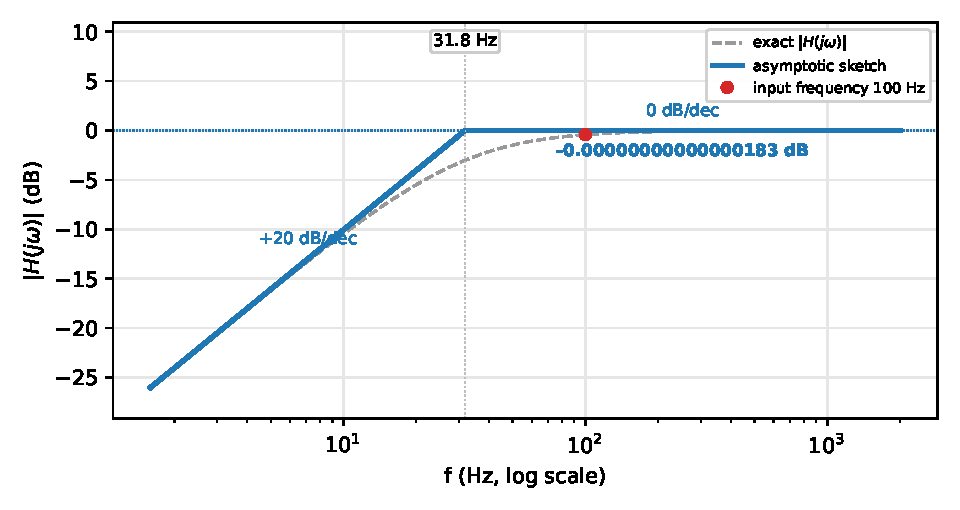
\includegraphics[width=0.78\linewidth,height=6.5cm,keepaspectratio]{p01_bode}\end{center}

{\small Blue: the straight-line sketch you are expected to draw. Dashed grey: the exact curve (about 3\,dB below the corner of an isolated pole). Red dot: the input frequency of Step 7.}
\solstep{7}{Steady-state output}The input is $V_i(t) = 0.5\sin\left(2\pi\cdot 100\,t\right)$, so $\omega_{in} = 2\pi\cdot 100 = 628$\,rad/s. Put $s=j\omega_{in}$ in each factor (tool T5): magnitudes multiply, angles add.
{\small Rules: $\left|\frac{s}{s+p}\right| = \frac{\omega}{\sqrt{\omega^2+p^2}}$, $\angle = \frac{\pi}{2}-\tan^{-1}\frac{\omega}{p}$;\quad $\left|\frac{1}{1+s/p}\right| = \frac{1}{\sqrt{1+(\omega/p)^2}}$, $\angle = -\tan^{-1}\frac{\omega}{p}$;\quad $\left|1+\frac{s}{z}\right| = \sqrt{1+(\omega/z)^2}$, $\angle = \tan^{-1}\frac{\omega}{z}$;\quad a negative $K$ adds $-\pi$.}
\begin{center}\renewcommand{\arraystretch}{1.35}
\begin{tabular}{ccc}
\toprule
factor & magnitude & angle (rad) \\
\midrule
$1$ & $1$ & $0$ \\
$\rule[-1.1em]{0pt}{2.8em}\dfrac{s}{s+2\pi\cdot 31.8}$ & $0.9529$ & $0.308$ \\
\textbf{total} & $\mathbf{0.9529}$ (product) & $\mathbf{0.308}$ (sum) \\
\bottomrule
\end{tabular}\end{center}

\begin{align*}
|H(j\omega_{in})| &= 0.953, \qquad \angle H(j\omega_{in}) = 0.308\ \mathrm{rad} \\
v_{o,ac}(t) &= 0.953\times 0.5\,\sin\left(2\pi\cdot 100\,t + 0.308\right) = 0.476\,\sin\left(2\pi\cdot 100\,t + 0.308\right)
\end{align*}

Add the DC part from Step 2 (superposition):
\[
\boxed{V_o(t) = 5 + 0.476\,\sin\left(2\pi\cdot 100\,t + 0.308\right)\ \mathrm{V}}
\]

\begin{ansbox}
$H(s) = 1\,\dfrac{s}{s+2\pi\cdot 31.8}$\quad (corners: 31.8 Hz)\\[4pt]
$V_o(t) = 5 + 0.476\,\sin\left(2\pi\cdot 100\,t + 0.308\right)\ \mathrm{V}$
\end{ansbox}

\newpage
\subsection*{Solution 1B.2 \hfill Easy}
\begin{center}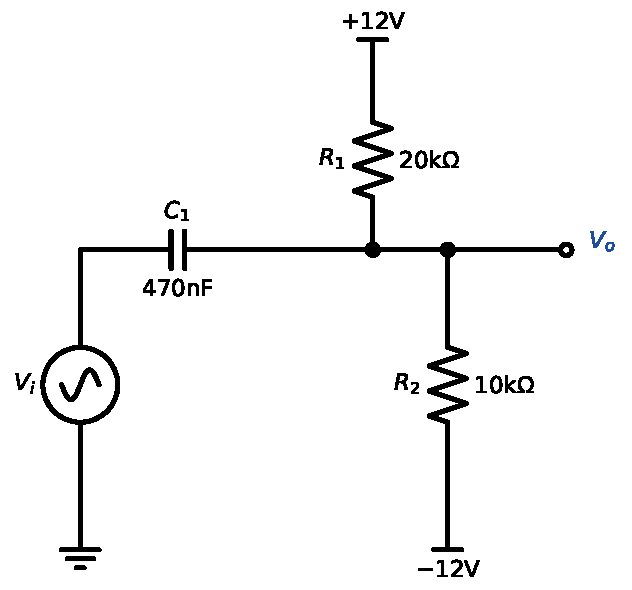
\includegraphics[width=0.8\linewidth,height=4.5cm,keepaspectratio]{p02_circuit}\end{center}
\solstep{1}{Identify the sources}Independent sources: the AC input $V_i(t)$ and the DC supplies $-12\,\mathrm{V}$, $+12\,\mathrm{V}$. Because there are both DC and AC sources, use superposition: $V_o(t) = V_{o,dc} + v_{o,ac}(t)$. Solve the DC circuit (Step 2) and the AC circuit (Steps 3--7) separately, then add.
\solstep{2}{DC circuit $\Rightarrow V_{o,dc}$}DC rules: the AC input is set to zero ($V_i=0$: a wire to ground); every capacitor is an open circuit ($C_{1}$). Only the part of the circuit that is still connected to $V_o$ matters:
\begin{center}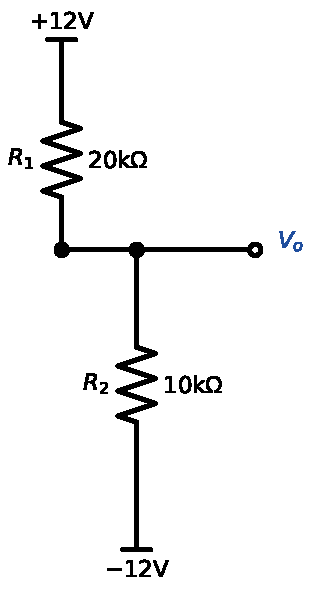
\includegraphics[width=0.55\linewidth,height=5cm,keepaspectratio]{p02_dc}\end{center}

Reduce the circuit with one tool only --- the \emph{divider between two voltages} (tool T3) --- walking toward $V_o$ and keeping a Thevenin pair $(V_{th},R_{th})$ for everything already visited.
\begin{enumerate}[leftmargin=*,itemsep=2pt]
\item Start at the input node: since $V_i=0$ it is tied to ground, i.e. it is an ideal $0\,\mathrm{V}$ source: $(V_{th},R_{th})=(0\,\mathrm{V},\,0\,\Omega)$.
\item $C_{1}$ is a capacitor $\Rightarrow$ open at DC. No DC current can cross it, so everything on its left is disconnected: start fresh after it.
\item Finally, collect everything at the output node $V_o$.
\item First DC path here: $R_{1}$ to the $+12\,\mathrm{V}$ supply, so $(V_{th},R_{th}) = (12\,\mathrm{V},\ 20\,\mathrm{k}\Omega)$.
\item Add $R_{2}$ to the $-12\,\mathrm{V}$ supply. Divider between $V_a=12\,\mathrm{V}$ (through $R_a=20\,\mathrm{k}\Omega$) and $V_b=-12\,\mathrm{V}$ (through $R_b=10\,\mathrm{k}\Omega$):\[
V_{th} = V_b + (V_a-V_b)\frac{R_b}{R_a+R_b} = -12 + \left(12 - (-12)\right)\frac{10\,\mathrm{k}}{20\,\mathrm{k} + 10\,\mathrm{k}} = -4\,\mathrm{V},\qquad R_{th} = R_a\parallel R_b = 6.67\,\mathrm{k}\Omega
\]

\end{enumerate}

\[
\boxed{V_{o,dc} = -4\,\mathrm{V}}
\]

\solstep{3}{AC circuit}Set every DC supply to zero: each supply rail becomes AC ground. Replace every capacitor by $\frac{1}{sC}$ and every inductor by $sL$.
\begin{itemize}[leftmargin=*,itemsep=2pt]
\item $R_{1}$, $R_{2}$ both go from the same node to (AC) ground, so they are in parallel: $R_{12} = R_{1} \parallel R_{2} = 20\,\mathrm{k} \parallel 10\,\mathrm{k} = 6.67\,\mathrm{k}\Omega$.
\end{itemize}

AC equivalent circuit (nodes named for the next step):
\begin{center}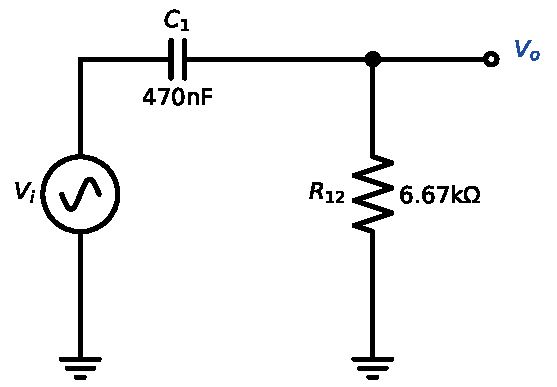
\includegraphics[width=0.95\linewidth,height=5.2cm,keepaspectratio]{p02_ac}\end{center}

\solstep{4}{Transfer function by a chain of dividers}Walk from the input to the output through the named nodes: $V_{i} \to V_{o}$. There is a single link, so $H(s)$ is just one voltage divider (tool T2).
Now each link. {\small (Algebra tip: to simplify a fraction that contains fractions, multiply its top and bottom by every inner denominator; then divide top and bottom by the leading coefficient of the denominator so that it starts with a plain $s^n$.)}
\begin{align*}
\frac{V_{o}}{V_{i}} &= \frac{R_{12}}{\frac{1}{sC_{1}} + R_{12}} = \dfrac{s}{s + 319}
\end{align*}

So:\[
H(s) = \dfrac{s}{s + 319}
\]

\solstep{5}{Standard (Bode-ready) form}Find the roots. Every root $s=-p$ of the denominator is a \emph{pole}, every root $s=-z$ of the numerator is a \emph{zero}; $|p|$ and $|z|$ are the corner frequencies (rad/s).
\begin{itemize}[leftmargin=*,itemsep=2pt]
\item Numerator: it has the factor $s$ $\Rightarrow$ 1 zero at $s=0$.
\item Denominator: $s + 319$; $s + 319 = 0 \Rightarrow s = -319$.
\end{itemize}

Factored form (leading coefficient in front):
\[
H(s) = 1\,\dfrac{s}{(s+319)}
\]

Bode-ready form: rewrite every $(s+p) = p\left(1+\frac{s}{p}\right)$ and $(s+z) = z\left(1+\frac{s}{z}\right)$, and collect all constants into $K$. Each $s$ in the numerator is paired with one of the \emph{lowest} poles as $\frac{s}{s+p}$ (that factor is $\approx 1$ above $p$). Then every factor except $K$ is $\approx 1$ inside the pass-band:
\[
H(s) = 1\,\dfrac{s}{s+2\pi\cdot 50.8},\qquad K = 1
\]

\begin{center}\renewcommand{\arraystretch}{1.35}
\begin{tabular}{cccc}
\toprule
type & $\omega_c$ (rad/s) & $f_c=\omega_c/2\pi$ & slope change \\
\midrule
pole & $319$ & 50.8 Hz & $-20$ dB/dec \\
\bottomrule
\end{tabular}\end{center}

\solstep{6}{Magnitude Bode plot}Below every corner $|H(s)|\approx 0.00313\,s$, so the plot starts with a slope of $+20$\,dB/dec. Then, moving right, each pole bends the line down by 20\,dB/dec and each zero bends it up by 20\,dB/dec (tool T6):
\begin{center}\renewcommand{\arraystretch}{1.35}
\begin{tabular}{lcl}
\toprule
frequency range & slope & asymptote level \\
\midrule
$f<$ 50.8 Hz & $+20$ dB/dec & 0 dB at end \\
$f>$ 50.8 Hz & $0$ dB/dec (flat) & 0 dB at start \\
\bottomrule
\end{tabular}\end{center}

The flat (pass-band) level is $20\log_{10}|K| = 20\log_{10}1 = 0$\,dB.
\begin{center}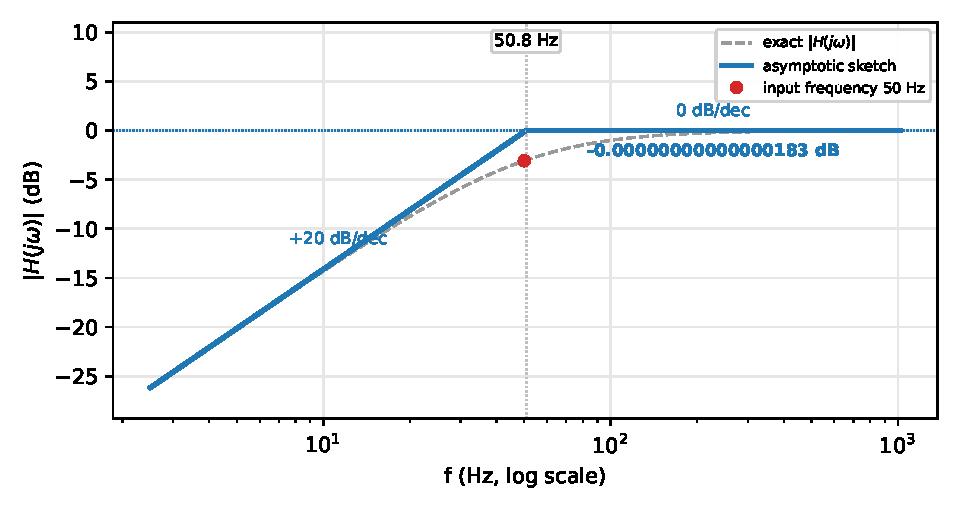
\includegraphics[width=0.78\linewidth,height=6.5cm,keepaspectratio]{p02_bode}\end{center}

{\small Blue: the straight-line sketch you are expected to draw. Dashed grey: the exact curve (about 3\,dB below the corner of an isolated pole). Red dot: the input frequency of Step 7.}
\solstep{7}{Steady-state output}The input is $V_i(t) = 1\sin\left(2\pi\cdot 50\,t\right)$, so $\omega_{in} = 2\pi\cdot 50 = 314$\,rad/s. Put $s=j\omega_{in}$ in each factor (tool T5): magnitudes multiply, angles add.
{\small Rules: $\left|\frac{s}{s+p}\right| = \frac{\omega}{\sqrt{\omega^2+p^2}}$, $\angle = \frac{\pi}{2}-\tan^{-1}\frac{\omega}{p}$;\quad $\left|\frac{1}{1+s/p}\right| = \frac{1}{\sqrt{1+(\omega/p)^2}}$, $\angle = -\tan^{-1}\frac{\omega}{p}$;\quad $\left|1+\frac{s}{z}\right| = \sqrt{1+(\omega/z)^2}$, $\angle = \tan^{-1}\frac{\omega}{z}$;\quad a negative $K$ adds $-\pi$.}
\begin{center}\renewcommand{\arraystretch}{1.35}
\begin{tabular}{ccc}
\toprule
factor & magnitude & angle (rad) \\
\midrule
$1$ & $1$ & $0$ \\
$\rule[-1.1em]{0pt}{2.8em}\dfrac{s}{s+2\pi\cdot 50.8}$ & $0.7015$ & $0.793$ \\
\textbf{total} & $\mathbf{0.7015}$ (product) & $\mathbf{0.793}$ (sum) \\
\bottomrule
\end{tabular}\end{center}

\begin{align*}
|H(j\omega_{in})| &= 0.702, \qquad \angle H(j\omega_{in}) = 0.793\ \mathrm{rad} \\
v_{o,ac}(t) &= 0.702\times 1\,\sin\left(2\pi\cdot 50\,t + 0.793\right) = 0.702\,\sin\left(2\pi\cdot 50\,t + 0.793\right)
\end{align*}

Add the DC part from Step 2 (superposition):
\[
\boxed{V_o(t) = -4 + 0.702\,\sin\left(2\pi\cdot 50\,t + 0.793\right)\ \mathrm{V}}
\]

\begin{ansbox}
$H(s) = 1\,\dfrac{s}{s+2\pi\cdot 50.8}$\quad (corners: 50.8 Hz)\\[4pt]
$V_o(t) = -4 + 0.702\,\sin\left(2\pi\cdot 50\,t + 0.793\right)\ \mathrm{V}$
\end{ansbox}

\newpage
\subsection*{Solution 1B.3 \hfill Easy}
\begin{center}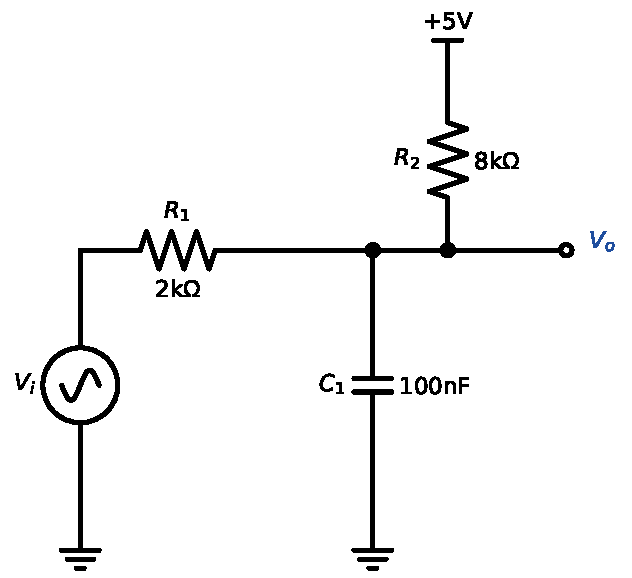
\includegraphics[width=0.8\linewidth,height=4.5cm,keepaspectratio]{p03_circuit}\end{center}
\solstep{1}{Identify the sources}Independent sources: the AC input $V_i(t)$ and the DC supplies $+5\,\mathrm{V}$. Because there are both DC and AC sources, use superposition: $V_o(t) = V_{o,dc} + v_{o,ac}(t)$. Solve the DC circuit (Step 2) and the AC circuit (Steps 3--7) separately, then add.
\solstep{2}{DC circuit $\Rightarrow V_{o,dc}$}DC rules: the AC input is set to zero ($V_i=0$: a wire to ground); every capacitor is an open circuit ($C_{1}$). Only the part of the circuit that is still connected to $V_o$ matters:
\begin{center}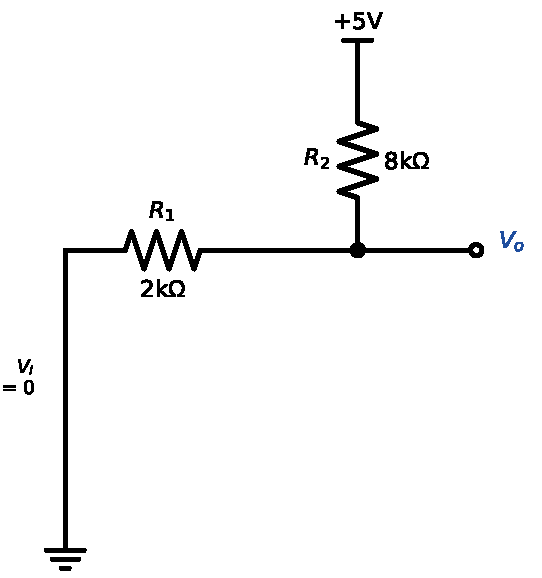
\includegraphics[width=0.55\linewidth,height=5cm,keepaspectratio]{p03_dc}\end{center}

Reduce the circuit with one tool only --- the \emph{divider between two voltages} (tool T3) --- walking toward $V_o$ and keeping a Thevenin pair $(V_{th},R_{th})$ for everything already visited.
\begin{enumerate}[leftmargin=*,itemsep=2pt]
\item Start at the input node: since $V_i=0$ it is tied to ground, i.e. it is an ideal $0\,\mathrm{V}$ source: $(V_{th},R_{th})=(0\,\mathrm{V},\,0\,\Omega)$.
\item Walk through $R_{1}$ ($2\,\mathrm{k}\Omega$ at DC). A series resistor just adds to $R_{th}$: $(V_{th},R_{th}) = (0\,\mathrm{V},\ 2\,\mathrm{k}\Omega)$.
\item Finally, collect everything at the output node $V_o$.
\item $C_{1}$ (at $V_{o}$) is a capacitor: open at DC, ignore it.
\item Add $R_{2}$ to the $+5\,\mathrm{V}$ supply. Divider between $V_a=0\,\mathrm{V}$ (through $R_a=2\,\mathrm{k}\Omega$) and $V_b=5\,\mathrm{V}$ (through $R_b=8\,\mathrm{k}\Omega$):\[
V_{th} = V_b + (V_a-V_b)\frac{R_b}{R_a+R_b} = 5 + \left(0 - (5)\right)\frac{8\,\mathrm{k}}{2\,\mathrm{k} + 8\,\mathrm{k}} = 1\,\mathrm{V},\qquad R_{th} = R_a\parallel R_b = 1.6\,\mathrm{k}\Omega
\]

\end{enumerate}

\[
\boxed{V_{o,dc} = 1\,\mathrm{V}}
\]

\solstep{3}{AC circuit}Set every DC supply to zero: each supply rail becomes AC ground. Replace every capacitor by $\frac{1}{sC}$ and every inductor by $sL$.
AC equivalent circuit (nodes named for the next step):
\begin{center}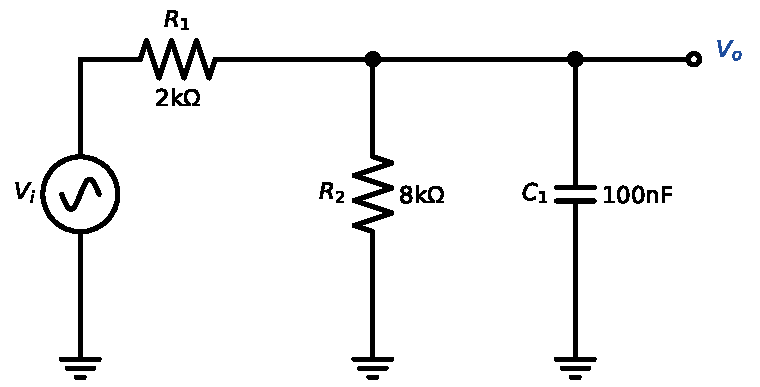
\includegraphics[width=0.95\linewidth,height=5.2cm,keepaspectratio]{p03_ac}\end{center}

\solstep{4}{Transfer function by a chain of dividers}Walk from the input to the output through the named nodes: $V_{i} \to V_{o}$. There is a single link, so $H(s)$ is just one voltage divider (tool T2).
Impedances seen \emph{looking right} from a node (everything from that node to ground, excluding what is on its left). Compute them from the far right toward the input:
\begin{align*}
Z_{o} &= R_{2} \parallel \frac{1}{sC_{1}} = \dfrac{10^{7}}{s + 1250}
\end{align*}

Now each link. {\small (Algebra tip: to simplify a fraction that contains fractions, multiply its top and bottom by every inner denominator; then divide top and bottom by the leading coefficient of the denominator so that it starts with a plain $s^n$.)}
\begin{align*}
\frac{V_{o}}{V_{i}} &= \frac{Z_{o}}{R_{1} + Z_{o}} = \dfrac{5000}{s + 6250}
\end{align*}

So:\[
H(s) = \dfrac{5000}{s + 6250}
\]

\solstep{5}{Standard (Bode-ready) form}Find the roots. Every root $s=-p$ of the denominator is a \emph{pole}, every root $s=-z$ of the numerator is a \emph{zero}; $|p|$ and $|z|$ are the corner frequencies (rad/s).
\begin{itemize}[leftmargin=*,itemsep=2pt]
\item Denominator: $s + 6250$; $s + 6250 = 0 \Rightarrow s = -6250$.
\end{itemize}

Factored form (leading coefficient in front):
\[
H(s) = 5000\,\dfrac{1}{(s+6250)}
\]

Bode-ready form: rewrite every $(s+p) = p\left(1+\frac{s}{p}\right)$ and $(s+z) = z\left(1+\frac{s}{z}\right)$, and collect all constants into $K$. Then every factor except $K$ is $\approx 1$ inside the pass-band:
\[
H(s) = 0.8\,\dfrac{1}{1+\dfrac{s}{2\pi\cdot 995}},\qquad K = 0.8
\]

\begin{center}\renewcommand{\arraystretch}{1.35}
\begin{tabular}{cccc}
\toprule
type & $\omega_c$ (rad/s) & $f_c=\omega_c/2\pi$ & slope change \\
\midrule
pole & $6250$ & 995 Hz & $-20$ dB/dec \\
\bottomrule
\end{tabular}\end{center}

\solstep{6}{Magnitude Bode plot}Below every corner, all factors are $\approx$ constant: $|H| \approx 0.8$ $= -1.94$\,dB (flat, 0 dB/dec). Then, moving right, each pole bends the line down by 20\,dB/dec and each zero bends it up by 20\,dB/dec (tool T6):
\begin{center}\renewcommand{\arraystretch}{1.35}
\begin{tabular}{lcl}
\toprule
frequency range & slope & asymptote level \\
\midrule
$f<$ 995 Hz & $0$ dB/dec (flat) & -1.94 dB at end \\
$f>$ 995 Hz & $-20$ dB/dec & -1.94 dB at start \\
\bottomrule
\end{tabular}\end{center}

The flat (pass-band) level is $20\log_{10}|K| = 20\log_{10}0.8 = -1.94$\,dB.
\begin{center}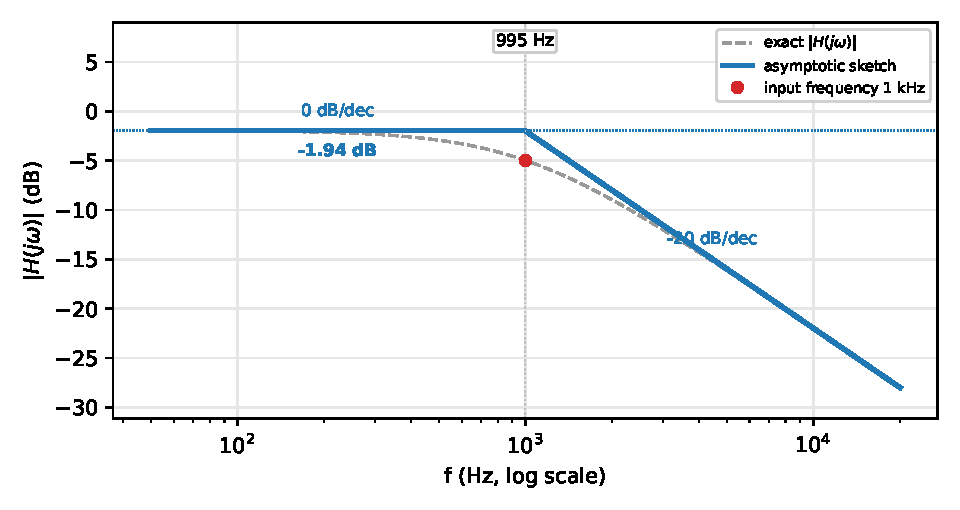
\includegraphics[width=0.78\linewidth,height=6.5cm,keepaspectratio]{p03_bode}\end{center}

{\small Blue: the straight-line sketch you are expected to draw. Dashed grey: the exact curve (about 3\,dB below the corner of an isolated pole). Red dot: the input frequency of Step 7.}
\solstep{7}{Steady-state output}The input is $V_i(t) = 0.5\sin\left(2\pi\cdot 1000\,t\right)$, so $\omega_{in} = 2\pi\cdot 1000 = 6280$\,rad/s. Put $s=j\omega_{in}$ in each factor (tool T5): magnitudes multiply, angles add.
{\small Rules: $\left|\frac{s}{s+p}\right| = \frac{\omega}{\sqrt{\omega^2+p^2}}$, $\angle = \frac{\pi}{2}-\tan^{-1}\frac{\omega}{p}$;\quad $\left|\frac{1}{1+s/p}\right| = \frac{1}{\sqrt{1+(\omega/p)^2}}$, $\angle = -\tan^{-1}\frac{\omega}{p}$;\quad $\left|1+\frac{s}{z}\right| = \sqrt{1+(\omega/z)^2}$, $\angle = \tan^{-1}\frac{\omega}{z}$;\quad a negative $K$ adds $-\pi$.}
\begin{center}\renewcommand{\arraystretch}{1.35}
\begin{tabular}{ccc}
\toprule
factor & magnitude & angle (rad) \\
\midrule
$0.8$ & $0.8$ & $0$ \\
$\rule[-1.7em]{0pt}{4em}\dfrac{1}{1+\dfrac{s}{2\pi\cdot 995}}$ & $0.7052$ & $-0.788$ \\
\textbf{total} & $\mathbf{0.5642}$ (product) & $\mathbf{-0.788}$ (sum) \\
\bottomrule
\end{tabular}\end{center}

\begin{align*}
|H(j\omega_{in})| &= 0.564, \qquad \angle H(j\omega_{in}) = -0.788\ \mathrm{rad} \\
v_{o,ac}(t) &= 0.564\times 0.5\,\sin\left(2\pi\cdot 1000\,t - 0.788\right) = 0.282\,\sin\left(2\pi\cdot 1000\,t - 0.788\right)
\end{align*}

Add the DC part from Step 2 (superposition):
\[
\boxed{V_o(t) = 1 + 0.282\,\sin\left(2\pi\cdot 1000\,t - 0.788\right)\ \mathrm{V}}
\]

\begin{ansbox}
$H(s) = 0.8\,\dfrac{1}{1+\dfrac{s}{2\pi\cdot 995}}$\quad (corners: 995 Hz)\\[4pt]
$V_o(t) = 1 + 0.282\,\sin\left(2\pi\cdot 1000\,t - 0.788\right)\ \mathrm{V}$
\end{ansbox}

\newpage
\subsection*{Solution 1B.4 \hfill Easy}
\begin{center}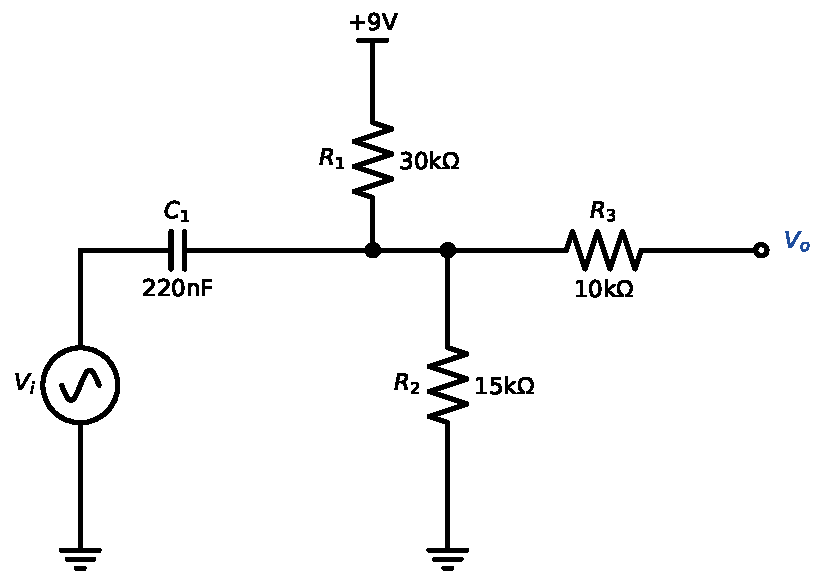
\includegraphics[width=0.8\linewidth,height=4.5cm,keepaspectratio]{p04_circuit}\end{center}
\solstep{1}{Identify the sources}Independent sources: the AC input $V_i(t)$ and the DC supplies $+9\,\mathrm{V}$. Because there are both DC and AC sources, use superposition: $V_o(t) = V_{o,dc} + v_{o,ac}(t)$. Solve the DC circuit (Step 2) and the AC circuit (Steps 3--7) separately, then add.
\solstep{2}{DC circuit $\Rightarrow V_{o,dc}$}DC rules: the AC input is set to zero ($V_i=0$: a wire to ground); every capacitor is an open circuit ($C_{1}$). Only the part of the circuit that is still connected to $V_o$ matters:
\begin{center}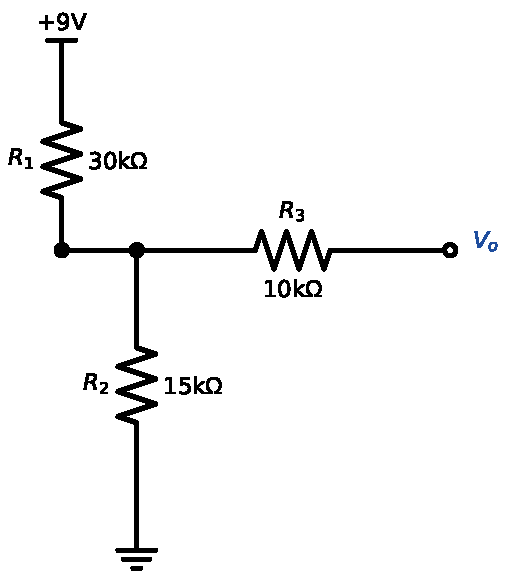
\includegraphics[width=0.55\linewidth,height=5cm,keepaspectratio]{p04_dc}\end{center}

Reduce the circuit with one tool only --- the \emph{divider between two voltages} (tool T3) --- walking toward $V_o$ and keeping a Thevenin pair $(V_{th},R_{th})$ for everything already visited.
\begin{enumerate}[leftmargin=*,itemsep=2pt]
\item Start at the input node: since $V_i=0$ it is tied to ground, i.e. it is an ideal $0\,\mathrm{V}$ source: $(V_{th},R_{th})=(0\,\mathrm{V},\,0\,\Omega)$.
\item $C_{1}$ is a capacitor $\Rightarrow$ open at DC. No DC current can cross it, so everything on its left is disconnected: start fresh after it.
\item First DC path here: $R_{1}$ to the $+9\,\mathrm{V}$ supply, so $(V_{th},R_{th}) = (9\,\mathrm{V},\ 30\,\mathrm{k}\Omega)$.
\item Add $R_{2}$ to ground. Divider between $V_a=9\,\mathrm{V}$ (through $R_a=30\,\mathrm{k}\Omega$) and $V_b=0\,\mathrm{V}$ (through $R_b=15\,\mathrm{k}\Omega$):\[
V_{th} = V_b + (V_a-V_b)\frac{R_b}{R_a+R_b} = 0 + \left(9 - (0)\right)\frac{15\,\mathrm{k}}{30\,\mathrm{k} + 15\,\mathrm{k}} = 3\,\mathrm{V},\qquad R_{th} = R_a\parallel R_b = 10\,\mathrm{k}\Omega
\]

\item Walk through $R_{3}$ ($10\,\mathrm{k}\Omega$ at DC). A series resistor just adds to $R_{th}$: $(V_{th},R_{th}) = (3\,\mathrm{V},\ 20\,\mathrm{k}\Omega)$.
\item Finally, collect everything at the output node $V_o$.
\item Nothing else draws DC current from $V_o$, so no current flows through $R_{th}$ and there is no voltage drop across it: $V_{o,dc}=V_{th}$.
\end{enumerate}

\[
\boxed{V_{o,dc} = 3\,\mathrm{V}}
\]

\solstep{3}{AC circuit}Set every DC supply to zero: each supply rail becomes AC ground. Replace every capacitor by $\frac{1}{sC}$ and every inductor by $sL$.
\begin{itemize}[leftmargin=*,itemsep=2pt]
\item $R_{1}$, $R_{2}$ both go from the same node to (AC) ground, so they are in parallel: $R_{12} = R_{1} \parallel R_{2} = 30\,\mathrm{k} \parallel 15\,\mathrm{k} = 10\,\mathrm{k}\Omega$.
\end{itemize}

AC equivalent circuit (nodes named for the next step):
\begin{center}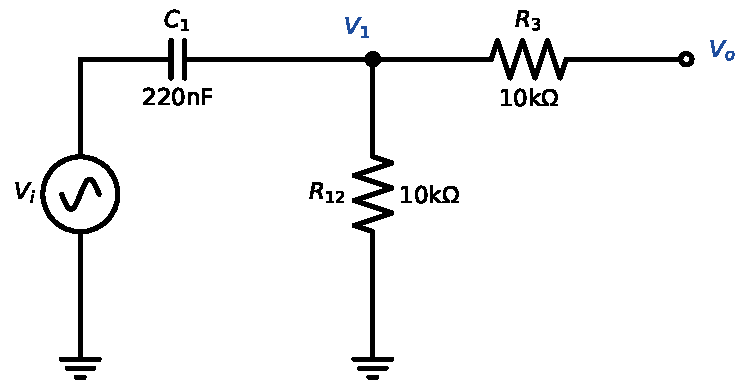
\includegraphics[width=0.95\linewidth,height=5.2cm,keepaspectratio]{p04_ac}\end{center}

\solstep{4}{Transfer function by a chain of dividers}Walk from the input to the output through the named nodes: $V_{i} \to V_{1} \to V_{o}$. The transfer function is the product of the node-to-node ratios (each one is a simple divider, tool T2, or a dependent source, tool T4):
\[
H(s) = \frac{V_o}{V_i} = \frac{V_{1}}{V_{i}}\cdot\frac{V_{o}}{V_{1}}
\]

Now each link. {\small (Algebra tip: to simplify a fraction that contains fractions, multiply its top and bottom by every inner denominator; then divide top and bottom by the leading coefficient of the denominator so that it starts with a plain $s^n$.)}
\begin{align*}
\frac{V_{1}}{V_{i}} &= \frac{R_{12}}{\frac{1}{sC_{1}} + R_{12}} = \dfrac{s}{s + 455} \\
\frac{V_{o}}{V_{1}} &= 1 &&\text{(nothing connected after $R_{3}$: no current, no drop)}
\end{align*}

Multiply the links and simplify (common factors cancel):\[
H(s) = \dfrac{s}{s + 455}
\]

\solstep{5}{Standard (Bode-ready) form}Find the roots. Every root $s=-p$ of the denominator is a \emph{pole}, every root $s=-z$ of the numerator is a \emph{zero}; $|p|$ and $|z|$ are the corner frequencies (rad/s).
\begin{itemize}[leftmargin=*,itemsep=2pt]
\item Numerator: it has the factor $s$ $\Rightarrow$ 1 zero at $s=0$.
\item Denominator: $s + 455$; $s + 455 = 0 \Rightarrow s = -455$.
\end{itemize}

Factored form (leading coefficient in front):
\[
H(s) = 1\,\dfrac{s}{(s+455)}
\]

Bode-ready form: rewrite every $(s+p) = p\left(1+\frac{s}{p}\right)$ and $(s+z) = z\left(1+\frac{s}{z}\right)$, and collect all constants into $K$. Each $s$ in the numerator is paired with one of the \emph{lowest} poles as $\frac{s}{s+p}$ (that factor is $\approx 1$ above $p$). Then every factor except $K$ is $\approx 1$ inside the pass-band:
\[
H(s) = 1\,\dfrac{s}{s+2\pi\cdot 72.3},\qquad K = 1
\]

\begin{center}\renewcommand{\arraystretch}{1.35}
\begin{tabular}{cccc}
\toprule
type & $\omega_c$ (rad/s) & $f_c=\omega_c/2\pi$ & slope change \\
\midrule
pole & $455$ & 72.3 Hz & $-20$ dB/dec \\
\bottomrule
\end{tabular}\end{center}

\solstep{6}{Magnitude Bode plot}Below every corner $|H(s)|\approx 0.0022\,s$, so the plot starts with a slope of $+20$\,dB/dec. Then, moving right, each pole bends the line down by 20\,dB/dec and each zero bends it up by 20\,dB/dec (tool T6):
\begin{center}\renewcommand{\arraystretch}{1.35}
\begin{tabular}{lcl}
\toprule
frequency range & slope & asymptote level \\
\midrule
$f<$ 72.3 Hz & $+20$ dB/dec & 0 dB at end \\
$f>$ 72.3 Hz & $0$ dB/dec (flat) & 0 dB at start \\
\bottomrule
\end{tabular}\end{center}

The flat (pass-band) level is $20\log_{10}|K| = 20\log_{10}1 = 0$\,dB.
\begin{center}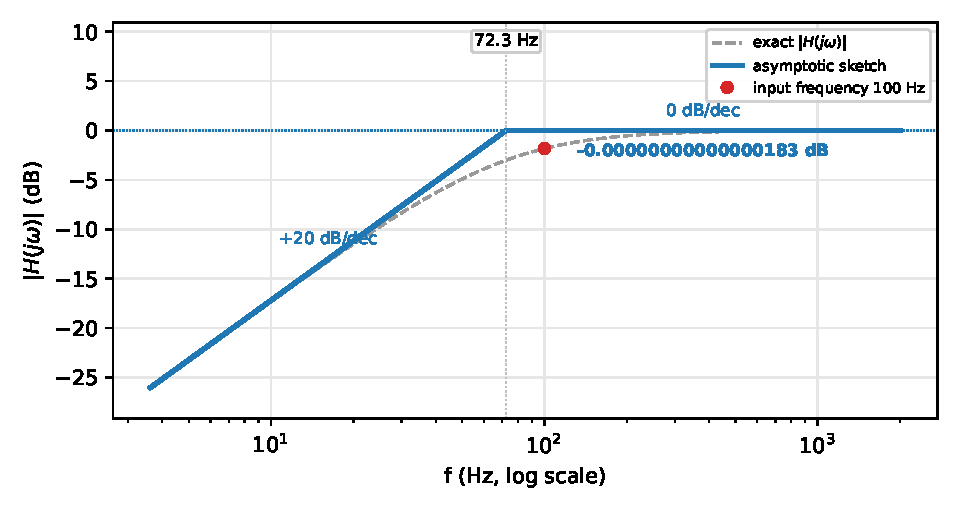
\includegraphics[width=0.78\linewidth,height=6.5cm,keepaspectratio]{p04_bode}\end{center}

{\small Blue: the straight-line sketch you are expected to draw. Dashed grey: the exact curve (about 3\,dB below the corner of an isolated pole). Red dot: the input frequency of Step 7.}
\solstep{7}{Steady-state output}The input is $V_i(t) = 0.2\sin\left(2\pi\cdot 100\,t\right)$, so $\omega_{in} = 2\pi\cdot 100 = 628$\,rad/s. Put $s=j\omega_{in}$ in each factor (tool T5): magnitudes multiply, angles add.
{\small Rules: $\left|\frac{s}{s+p}\right| = \frac{\omega}{\sqrt{\omega^2+p^2}}$, $\angle = \frac{\pi}{2}-\tan^{-1}\frac{\omega}{p}$;\quad $\left|\frac{1}{1+s/p}\right| = \frac{1}{\sqrt{1+(\omega/p)^2}}$, $\angle = -\tan^{-1}\frac{\omega}{p}$;\quad $\left|1+\frac{s}{z}\right| = \sqrt{1+(\omega/z)^2}$, $\angle = \tan^{-1}\frac{\omega}{z}$;\quad a negative $K$ adds $-\pi$.}
\begin{center}\renewcommand{\arraystretch}{1.35}
\begin{tabular}{ccc}
\toprule
factor & magnitude & angle (rad) \\
\midrule
$1$ & $1$ & $0$ \\
$\rule[-1.1em]{0pt}{2.8em}\dfrac{s}{s+2\pi\cdot 72.3}$ & $0.8102$ & $0.626$ \\
\textbf{total} & $\mathbf{0.8102}$ (product) & $\mathbf{0.626}$ (sum) \\
\bottomrule
\end{tabular}\end{center}

\begin{align*}
|H(j\omega_{in})| &= 0.81, \qquad \angle H(j\omega_{in}) = 0.626\ \mathrm{rad} \\
v_{o,ac}(t) &= 0.81\times 0.2\,\sin\left(2\pi\cdot 100\,t + 0.626\right) = 0.162\,\sin\left(2\pi\cdot 100\,t + 0.626\right)
\end{align*}

Add the DC part from Step 2 (superposition):
\[
\boxed{V_o(t) = 3 + 0.162\,\sin\left(2\pi\cdot 100\,t + 0.626\right)\ \mathrm{V}}
\]

\begin{ansbox}
$H(s) = 1\,\dfrac{s}{s+2\pi\cdot 72.3}$\quad (corners: 72.3 Hz)\\[4pt]
$V_o(t) = 3 + 0.162\,\sin\left(2\pi\cdot 100\,t + 0.626\right)\ \mathrm{V}$
\end{ansbox}

\newpage
\subsection*{Solution 1B.5 \hfill Easy}
\begin{center}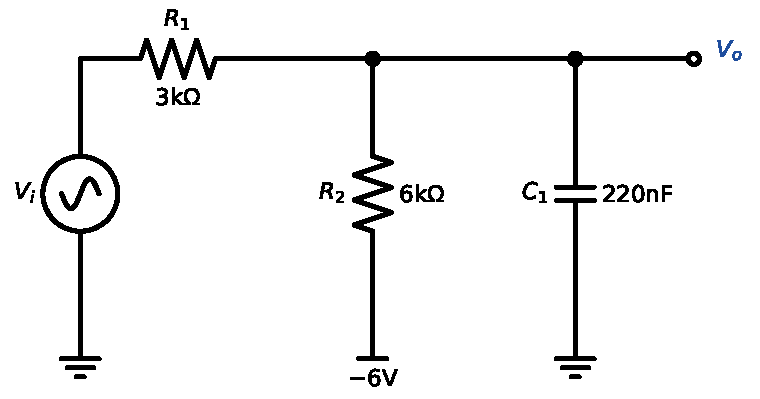
\includegraphics[width=0.8\linewidth,height=4.5cm,keepaspectratio]{p05_circuit}\end{center}
\solstep{1}{Identify the sources}Independent sources: the AC input $V_i(t)$ and the DC supplies $-6\,\mathrm{V}$. Because there are both DC and AC sources, use superposition: $V_o(t) = V_{o,dc} + v_{o,ac}(t)$. Solve the DC circuit (Step 2) and the AC circuit (Steps 3--7) separately, then add.
\solstep{2}{DC circuit $\Rightarrow V_{o,dc}$}DC rules: the AC input is set to zero ($V_i=0$: a wire to ground); every capacitor is an open circuit ($C_{1}$). Only the part of the circuit that is still connected to $V_o$ matters:
\begin{center}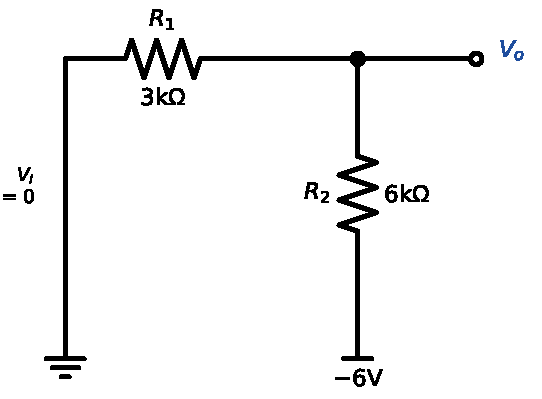
\includegraphics[width=0.55\linewidth,height=5cm,keepaspectratio]{p05_dc}\end{center}

Reduce the circuit with one tool only --- the \emph{divider between two voltages} (tool T3) --- walking toward $V_o$ and keeping a Thevenin pair $(V_{th},R_{th})$ for everything already visited.
\begin{enumerate}[leftmargin=*,itemsep=2pt]
\item Start at the input node: since $V_i=0$ it is tied to ground, i.e. it is an ideal $0\,\mathrm{V}$ source: $(V_{th},R_{th})=(0\,\mathrm{V},\,0\,\Omega)$.
\item Walk through $R_{1}$ ($3\,\mathrm{k}\Omega$ at DC). A series resistor just adds to $R_{th}$: $(V_{th},R_{th}) = (0\,\mathrm{V},\ 3\,\mathrm{k}\Omega)$.
\item Finally, collect everything at the output node $V_o$.
\item Add $R_{2}$ to the $-6\,\mathrm{V}$ supply. Divider between $V_a=0\,\mathrm{V}$ (through $R_a=3\,\mathrm{k}\Omega$) and $V_b=-6\,\mathrm{V}$ (through $R_b=6\,\mathrm{k}\Omega$):\[
V_{th} = V_b + (V_a-V_b)\frac{R_b}{R_a+R_b} = -6 + \left(0 - (-6)\right)\frac{6\,\mathrm{k}}{3\,\mathrm{k} + 6\,\mathrm{k}} = -2\,\mathrm{V},\qquad R_{th} = R_a\parallel R_b = 2\,\mathrm{k}\Omega
\]

\item $C_{1}$ (at $V_{o}$) is a capacitor: open at DC, ignore it.
\end{enumerate}

\[
\boxed{V_{o,dc} = -2\,\mathrm{V}}
\]

\solstep{3}{AC circuit}Set every DC supply to zero: each supply rail becomes AC ground. Replace every capacitor by $\frac{1}{sC}$ and every inductor by $sL$.
AC equivalent circuit (nodes named for the next step):
\begin{center}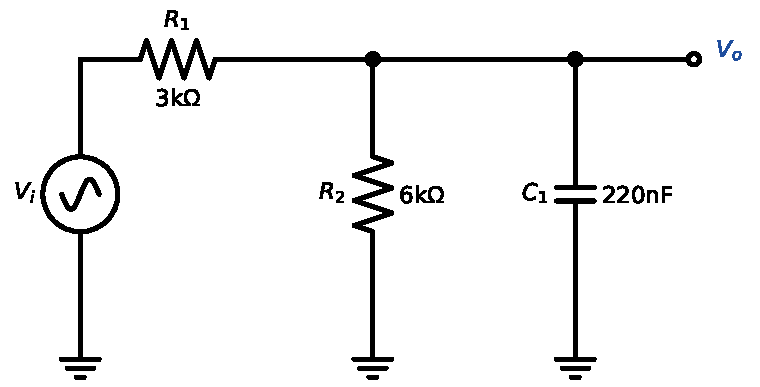
\includegraphics[width=0.95\linewidth,height=5.2cm,keepaspectratio]{p05_ac}\end{center}

\solstep{4}{Transfer function by a chain of dividers}Walk from the input to the output through the named nodes: $V_{i} \to V_{o}$. There is a single link, so $H(s)$ is just one voltage divider (tool T2).
Impedances seen \emph{looking right} from a node (everything from that node to ground, excluding what is on its left). Compute them from the far right toward the input:
\begin{align*}
Z_{o} &= R_{2} \parallel \frac{1}{sC_{1}} = \dfrac{4.55\times 10^{6}}{s + 758}
\end{align*}

Now each link. {\small (Algebra tip: to simplify a fraction that contains fractions, multiply its top and bottom by every inner denominator; then divide top and bottom by the leading coefficient of the denominator so that it starts with a plain $s^n$.)}
\begin{align*}
\frac{V_{o}}{V_{i}} &= \frac{Z_{o}}{R_{1} + Z_{o}} = \dfrac{1520}{s + 2270}
\end{align*}

So:\[
H(s) = \dfrac{1520}{s + 2270}
\]

\solstep{5}{Standard (Bode-ready) form}Find the roots. Every root $s=-p$ of the denominator is a \emph{pole}, every root $s=-z$ of the numerator is a \emph{zero}; $|p|$ and $|z|$ are the corner frequencies (rad/s).
\begin{itemize}[leftmargin=*,itemsep=2pt]
\item Denominator: $s + 2270$; $s + 2270 = 0 \Rightarrow s = -2270$.
\end{itemize}

Factored form (leading coefficient in front):
\[
H(s) = 1520\,\dfrac{1}{(s+2270)}
\]

Bode-ready form: rewrite every $(s+p) = p\left(1+\frac{s}{p}\right)$ and $(s+z) = z\left(1+\frac{s}{z}\right)$, and collect all constants into $K$. Then every factor except $K$ is $\approx 1$ inside the pass-band:
\[
H(s) = 0.667\,\dfrac{1}{1+\dfrac{s}{2\pi\cdot 362}},\qquad K = 0.667
\]

\begin{center}\renewcommand{\arraystretch}{1.35}
\begin{tabular}{cccc}
\toprule
type & $\omega_c$ (rad/s) & $f_c=\omega_c/2\pi$ & slope change \\
\midrule
pole & $2270$ & 362 Hz & $-20$ dB/dec \\
\bottomrule
\end{tabular}\end{center}

\solstep{6}{Magnitude Bode plot}Below every corner, all factors are $\approx$ constant: $|H| \approx 0.667$ $= -3.52$\,dB (flat, 0 dB/dec). Then, moving right, each pole bends the line down by 20\,dB/dec and each zero bends it up by 20\,dB/dec (tool T6):
\begin{center}\renewcommand{\arraystretch}{1.35}
\begin{tabular}{lcl}
\toprule
frequency range & slope & asymptote level \\
\midrule
$f<$ 362 Hz & $0$ dB/dec (flat) & -3.52 dB at end \\
$f>$ 362 Hz & $-20$ dB/dec & -3.52 dB at start \\
\bottomrule
\end{tabular}\end{center}

The flat (pass-band) level is $20\log_{10}|K| = 20\log_{10}0.667 = -3.52$\,dB.
\begin{center}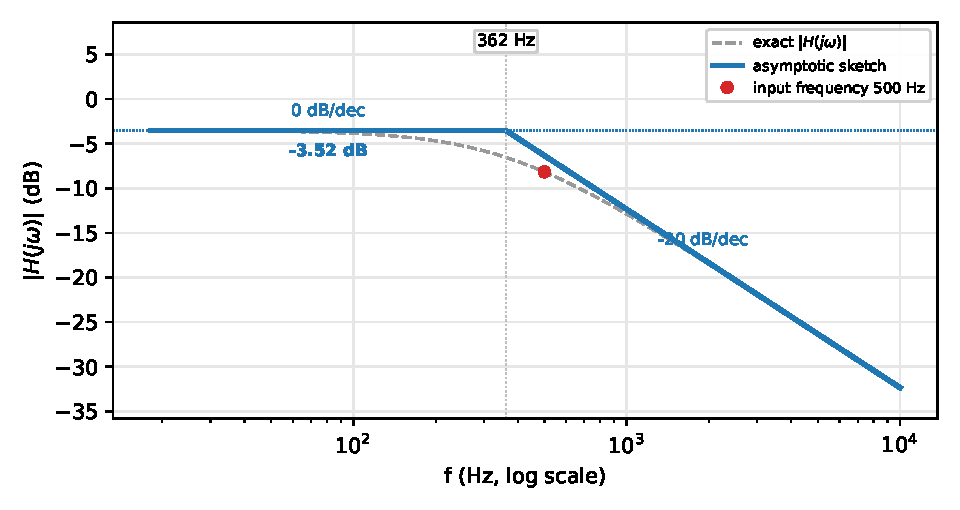
\includegraphics[width=0.78\linewidth,height=6.5cm,keepaspectratio]{p05_bode}\end{center}

{\small Blue: the straight-line sketch you are expected to draw. Dashed grey: the exact curve (about 3\,dB below the corner of an isolated pole). Red dot: the input frequency of Step 7.}
\solstep{7}{Steady-state output}The input is $V_i(t) = 1\sin\left(2\pi\cdot 500\,t\right)$, so $\omega_{in} = 2\pi\cdot 500 = 3140$\,rad/s. Put $s=j\omega_{in}$ in each factor (tool T5): magnitudes multiply, angles add.
{\small Rules: $\left|\frac{s}{s+p}\right| = \frac{\omega}{\sqrt{\omega^2+p^2}}$, $\angle = \frac{\pi}{2}-\tan^{-1}\frac{\omega}{p}$;\quad $\left|\frac{1}{1+s/p}\right| = \frac{1}{\sqrt{1+(\omega/p)^2}}$, $\angle = -\tan^{-1}\frac{\omega}{p}$;\quad $\left|1+\frac{s}{z}\right| = \sqrt{1+(\omega/z)^2}$, $\angle = \tan^{-1}\frac{\omega}{z}$;\quad a negative $K$ adds $-\pi$.}
\begin{center}\renewcommand{\arraystretch}{1.35}
\begin{tabular}{ccc}
\toprule
factor & magnitude & angle (rad) \\
\midrule
$0.667$ & $0.6667$ & $0$ \\
$\rule[-1.7em]{0pt}{4em}\dfrac{1}{1+\dfrac{s}{2\pi\cdot 362}}$ & $0.5861$ & $-0.945$ \\
\textbf{total} & $\mathbf{0.3908}$ (product) & $\mathbf{-0.945}$ (sum) \\
\bottomrule
\end{tabular}\end{center}

\begin{align*}
|H(j\omega_{in})| &= 0.391, \qquad \angle H(j\omega_{in}) = -0.945\ \mathrm{rad} \\
v_{o,ac}(t) &= 0.391\times 1\,\sin\left(2\pi\cdot 500\,t - 0.945\right) = 0.391\,\sin\left(2\pi\cdot 500\,t - 0.945\right)
\end{align*}

Add the DC part from Step 2 (superposition):
\[
\boxed{V_o(t) = -2 + 0.391\,\sin\left(2\pi\cdot 500\,t - 0.945\right)\ \mathrm{V}}
\]

\begin{ansbox}
$H(s) = 0.667\,\dfrac{1}{1+\dfrac{s}{2\pi\cdot 362}}$\quad (corners: 362 Hz)\\[4pt]
$V_o(t) = -2 + 0.391\,\sin\left(2\pi\cdot 500\,t - 0.945\right)\ \mathrm{V}$
\end{ansbox}

\newpage
\subsection*{Solution 1B.6 \hfill Easy}
\begin{center}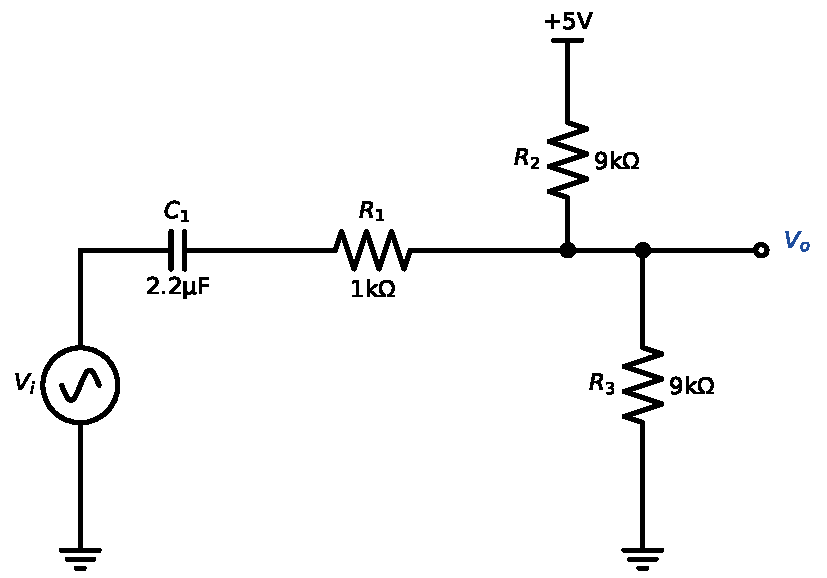
\includegraphics[width=0.8\linewidth,height=4.5cm,keepaspectratio]{p06_circuit}\end{center}
\solstep{1}{Identify the sources}Independent sources: the AC input $V_i(t)$ and the DC supplies $+5\,\mathrm{V}$. Because there are both DC and AC sources, use superposition: $V_o(t) = V_{o,dc} + v_{o,ac}(t)$. Solve the DC circuit (Step 2) and the AC circuit (Steps 3--7) separately, then add.
\solstep{2}{DC circuit $\Rightarrow V_{o,dc}$}DC rules: the AC input is set to zero ($V_i=0$: a wire to ground); every capacitor is an open circuit ($C_{1}$). Only the part of the circuit that is still connected to $V_o$ matters:
\begin{center}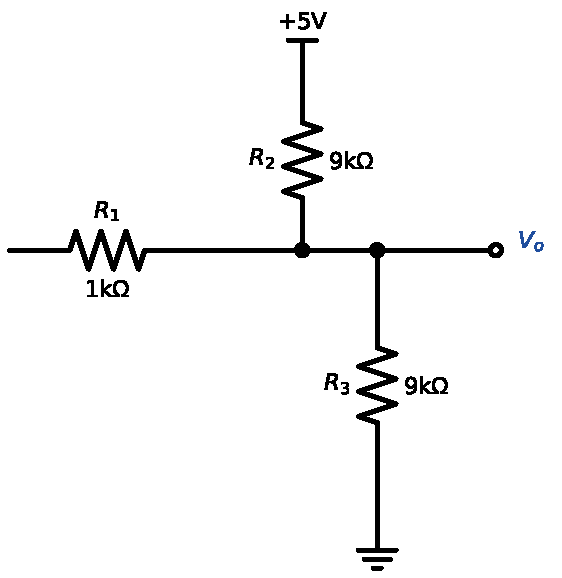
\includegraphics[width=0.55\linewidth,height=5cm,keepaspectratio]{p06_dc}\end{center}

Reduce the circuit with one tool only --- the \emph{divider between two voltages} (tool T3) --- walking toward $V_o$ and keeping a Thevenin pair $(V_{th},R_{th})$ for everything already visited.
\begin{enumerate}[leftmargin=*,itemsep=2pt]
\item Start at the input node: since $V_i=0$ it is tied to ground, i.e. it is an ideal $0\,\mathrm{V}$ source: $(V_{th},R_{th})=(0\,\mathrm{V},\,0\,\Omega)$.
\item $C_{1}$ is a capacitor $\Rightarrow$ open at DC. No DC current can cross it, so everything on its left is disconnected: start fresh after it.
\item Finally, collect everything at the output node $V_o$.
\item First DC path here: $R_{2}$ to the $+5\,\mathrm{V}$ supply, so $(V_{th},R_{th}) = (5\,\mathrm{V},\ 9\,\mathrm{k}\Omega)$.
\item Add $R_{3}$ to ground. Divider between $V_a=5\,\mathrm{V}$ (through $R_a=9\,\mathrm{k}\Omega$) and $V_b=0\,\mathrm{V}$ (through $R_b=9\,\mathrm{k}\Omega$):\[
V_{th} = V_b + (V_a-V_b)\frac{R_b}{R_a+R_b} = 0 + \left(5 - (0)\right)\frac{9\,\mathrm{k}}{9\,\mathrm{k} + 9\,\mathrm{k}} = 2.5\,\mathrm{V},\qquad R_{th} = R_a\parallel R_b = 4.5\,\mathrm{k}\Omega
\]

\end{enumerate}

\[
\boxed{V_{o,dc} = 2.5\,\mathrm{V}}
\]

\solstep{3}{AC circuit}Set every DC supply to zero: each supply rail becomes AC ground. Replace every capacitor by $\frac{1}{sC}$ and every inductor by $sL$.
\begin{itemize}[leftmargin=*,itemsep=2pt]
\item $R_{2}$, $R_{3}$ both go from the same node to (AC) ground, so they are in parallel: $R_{23} = R_{2} \parallel R_{3} = 9\,\mathrm{k} \parallel 9\,\mathrm{k} = 4.5\,\mathrm{k}\Omega$.
\end{itemize}

AC equivalent circuit (nodes named for the next step):
\begin{center}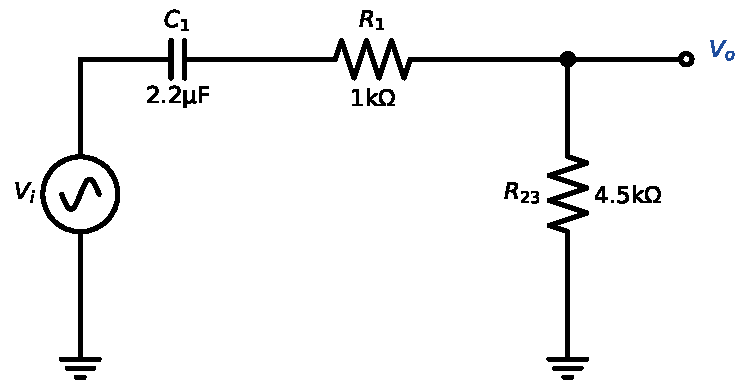
\includegraphics[width=0.95\linewidth,height=5.2cm,keepaspectratio]{p06_ac}\end{center}

\solstep{4}{Transfer function by a chain of dividers}Walk from the input to the output through the named nodes: $V_{i} \to V_{o}$. There is a single link, so $H(s)$ is just one voltage divider (tool T2).
Now each link. {\small (Algebra tip: to simplify a fraction that contains fractions, multiply its top and bottom by every inner denominator; then divide top and bottom by the leading coefficient of the denominator so that it starts with a plain $s^n$.)}
\begin{align*}
\frac{V_{o}}{V_{i}} &= \frac{R_{23}}{\frac{1}{sC_{1}} + R_{1} + R_{23}} = \dfrac{0.818\,s}{s + 82.6}
\end{align*}

So:\[
H(s) = \dfrac{0.818\,s}{s + 82.6}
\]

\solstep{5}{Standard (Bode-ready) form}Find the roots. Every root $s=-p$ of the denominator is a \emph{pole}, every root $s=-z$ of the numerator is a \emph{zero}; $|p|$ and $|z|$ are the corner frequencies (rad/s).
\begin{itemize}[leftmargin=*,itemsep=2pt]
\item Numerator: it has the factor $s$ $\Rightarrow$ 1 zero at $s=0$.
\item Denominator: $s + 82.6$; $s + 82.6 = 0 \Rightarrow s = -82.6$.
\end{itemize}

Factored form (leading coefficient in front):
\[
H(s) = 0.818\,\dfrac{s}{(s+82.6)}
\]

Bode-ready form: rewrite every $(s+p) = p\left(1+\frac{s}{p}\right)$ and $(s+z) = z\left(1+\frac{s}{z}\right)$, and collect all constants into $K$. Each $s$ in the numerator is paired with one of the \emph{lowest} poles as $\frac{s}{s+p}$ (that factor is $\approx 1$ above $p$). Then every factor except $K$ is $\approx 1$ inside the pass-band:
\[
H(s) = 0.818\,\dfrac{s}{s+2\pi\cdot 13.2},\qquad K = 0.818
\]

\begin{center}\renewcommand{\arraystretch}{1.35}
\begin{tabular}{cccc}
\toprule
type & $\omega_c$ (rad/s) & $f_c=\omega_c/2\pi$ & slope change \\
\midrule
pole & $82.6$ & 13.2 Hz & $-20$ dB/dec \\
\bottomrule
\end{tabular}\end{center}

\solstep{6}{Magnitude Bode plot}Below every corner $|H(s)|\approx 0.0099\,s$, so the plot starts with a slope of $+20$\,dB/dec. Then, moving right, each pole bends the line down by 20\,dB/dec and each zero bends it up by 20\,dB/dec (tool T6):
\begin{center}\renewcommand{\arraystretch}{1.35}
\begin{tabular}{lcl}
\toprule
frequency range & slope & asymptote level \\
\midrule
$f<$ 13.2 Hz & $+20$ dB/dec & -1.74 dB at end \\
$f>$ 13.2 Hz & $0$ dB/dec (flat) & -1.74 dB at start \\
\bottomrule
\end{tabular}\end{center}

The flat (pass-band) level is $20\log_{10}|K| = 20\log_{10}0.818 = -1.74$\,dB.
\begin{center}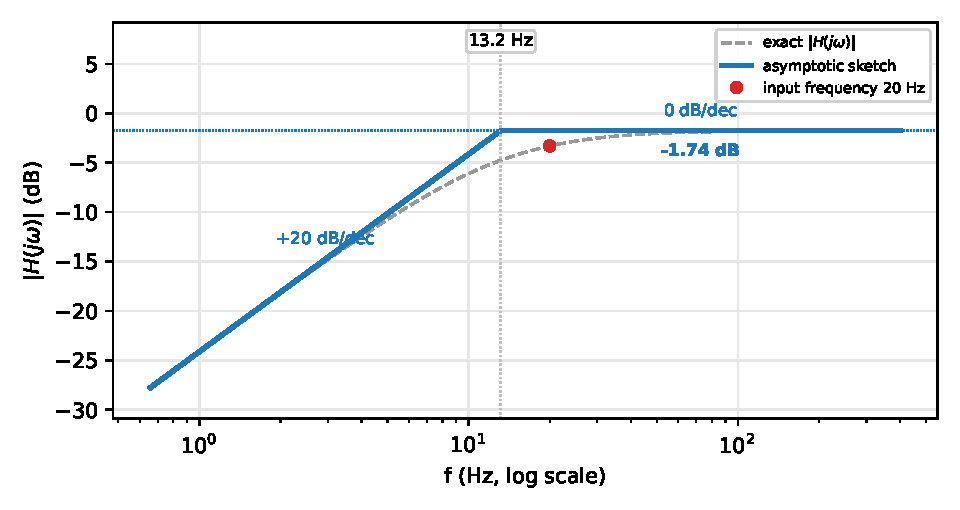
\includegraphics[width=0.78\linewidth,height=6.5cm,keepaspectratio]{p06_bode}\end{center}

{\small Blue: the straight-line sketch you are expected to draw. Dashed grey: the exact curve (about 3\,dB below the corner of an isolated pole). Red dot: the input frequency of Step 7.}
\solstep{7}{Steady-state output}The input is $V_i(t) = 0.3\sin\left(2\pi\cdot 20\,t\right)$, so $\omega_{in} = 2\pi\cdot 20 = 126$\,rad/s. Put $s=j\omega_{in}$ in each factor (tool T5): magnitudes multiply, angles add.
{\small Rules: $\left|\frac{s}{s+p}\right| = \frac{\omega}{\sqrt{\omega^2+p^2}}$, $\angle = \frac{\pi}{2}-\tan^{-1}\frac{\omega}{p}$;\quad $\left|\frac{1}{1+s/p}\right| = \frac{1}{\sqrt{1+(\omega/p)^2}}$, $\angle = -\tan^{-1}\frac{\omega}{p}$;\quad $\left|1+\frac{s}{z}\right| = \sqrt{1+(\omega/z)^2}$, $\angle = \tan^{-1}\frac{\omega}{z}$;\quad a negative $K$ adds $-\pi$.}
\begin{center}\renewcommand{\arraystretch}{1.35}
\begin{tabular}{ccc}
\toprule
factor & magnitude & angle (rad) \\
\midrule
$0.818$ & $0.8182$ & $0$ \\
$\rule[-1.1em]{0pt}{2.8em}\dfrac{s}{s+2\pi\cdot 13.2}$ & $0.8355$ & $0.582$ \\
\textbf{total} & $\mathbf{0.6836}$ (product) & $\mathbf{0.582}$ (sum) \\
\bottomrule
\end{tabular}\end{center}

\begin{align*}
|H(j\omega_{in})| &= 0.684, \qquad \angle H(j\omega_{in}) = 0.582\ \mathrm{rad} \\
v_{o,ac}(t) &= 0.684\times 0.3\,\sin\left(2\pi\cdot 20\,t + 0.582\right) = 0.205\,\sin\left(2\pi\cdot 20\,t + 0.582\right)
\end{align*}

Add the DC part from Step 2 (superposition):
\[
\boxed{V_o(t) = 2.5 + 0.205\,\sin\left(2\pi\cdot 20\,t + 0.582\right)\ \mathrm{V}}
\]

\begin{ansbox}
$H(s) = 0.818\,\dfrac{s}{s+2\pi\cdot 13.2}$\quad (corners: 13.2 Hz)\\[4pt]
$V_o(t) = 2.5 + 0.205\,\sin\left(2\pi\cdot 20\,t + 0.582\right)\ \mathrm{V}$
\end{ansbox}

\newpage
\subsection*{Solution 1B.7 \hfill Medium}
\begin{center}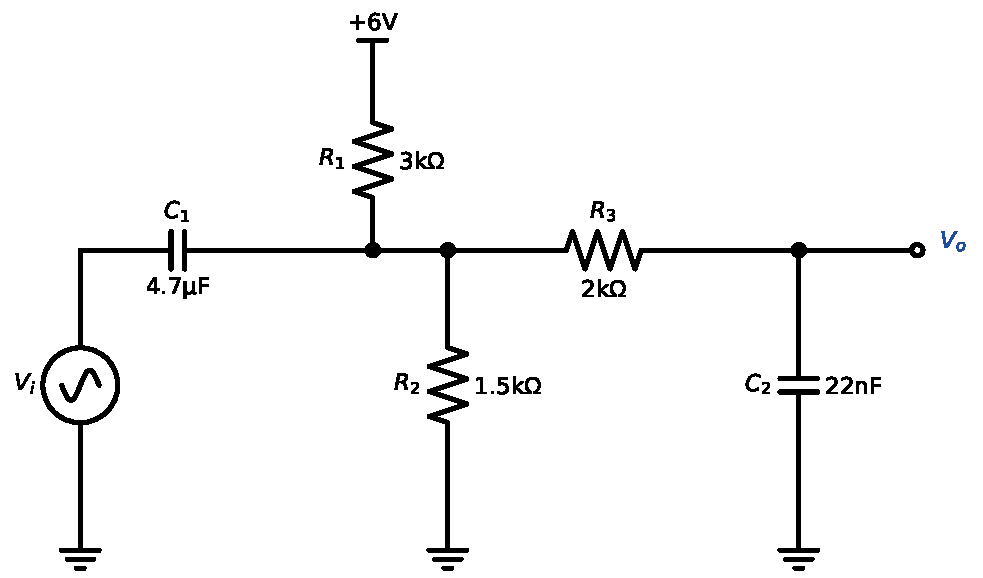
\includegraphics[width=0.8\linewidth,height=4.5cm,keepaspectratio]{p07_circuit}\end{center}
\solstep{1}{Identify the sources}Independent sources: the AC input $V_i(t)$ and the DC supplies $+6\,\mathrm{V}$. Because there are both DC and AC sources, use superposition: $V_o(t) = V_{o,dc} + v_{o,ac}(t)$. Solve the DC circuit (Step 2) and the AC circuit (Steps 3--7) separately, then add.
\solstep{2}{DC circuit $\Rightarrow V_{o,dc}$}DC rules: the AC input is set to zero ($V_i=0$: a wire to ground); every capacitor is an open circuit ($C_{1}, C_{2}$). Only the part of the circuit that is still connected to $V_o$ matters:
\begin{center}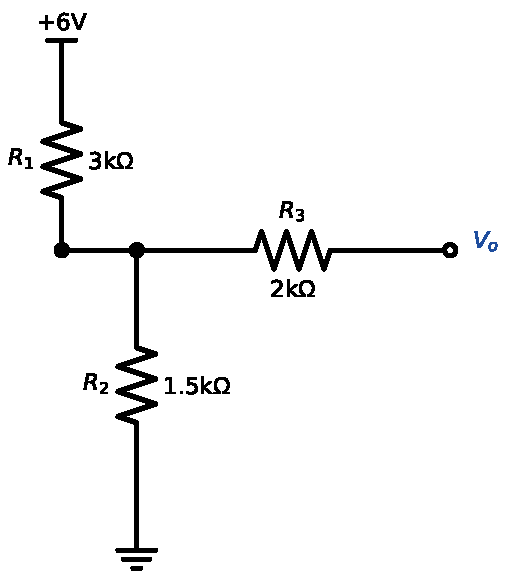
\includegraphics[width=0.55\linewidth,height=5cm,keepaspectratio]{p07_dc}\end{center}

Reduce the circuit with one tool only --- the \emph{divider between two voltages} (tool T3) --- walking toward $V_o$ and keeping a Thevenin pair $(V_{th},R_{th})$ for everything already visited.
\begin{enumerate}[leftmargin=*,itemsep=2pt]
\item Start at the input node: since $V_i=0$ it is tied to ground, i.e. it is an ideal $0\,\mathrm{V}$ source: $(V_{th},R_{th})=(0\,\mathrm{V},\,0\,\Omega)$.
\item $C_{1}$ is a capacitor $\Rightarrow$ open at DC. No DC current can cross it, so everything on its left is disconnected: start fresh after it.
\item First DC path here: $R_{1}$ to the $+6\,\mathrm{V}$ supply, so $(V_{th},R_{th}) = (6\,\mathrm{V},\ 3\,\mathrm{k}\Omega)$.
\item Add $R_{2}$ to ground. Divider between $V_a=6\,\mathrm{V}$ (through $R_a=3\,\mathrm{k}\Omega$) and $V_b=0\,\mathrm{V}$ (through $R_b=1.5\,\mathrm{k}\Omega$):\[
V_{th} = V_b + (V_a-V_b)\frac{R_b}{R_a+R_b} = 0 + \left(6 - (0)\right)\frac{1.5\,\mathrm{k}}{3\,\mathrm{k} + 1.5\,\mathrm{k}} = 2\,\mathrm{V},\qquad R_{th} = R_a\parallel R_b = 1\,\mathrm{k}\Omega
\]

\item Walk through $R_{3}$ ($2\,\mathrm{k}\Omega$ at DC). A series resistor just adds to $R_{th}$: $(V_{th},R_{th}) = (2\,\mathrm{V},\ 3\,\mathrm{k}\Omega)$.
\item Finally, collect everything at the output node $V_o$.
\item $C_{2}$ (at $V_{o}$) is a capacitor: open at DC, ignore it.
\item Nothing else draws DC current from $V_o$, so no current flows through $R_{th}$ and there is no voltage drop across it: $V_{o,dc}=V_{th}$.
\end{enumerate}

\[
\boxed{V_{o,dc} = 2\,\mathrm{V}}
\]

\solstep{3}{AC circuit}Set every DC supply to zero: each supply rail becomes AC ground. Replace every capacitor by $\frac{1}{sC}$ and every inductor by $sL$.
\begin{itemize}[leftmargin=*,itemsep=2pt]
\item $R_{1}$, $R_{2}$ both go from the same node to (AC) ground, so they are in parallel: $R_{12} = R_{1} \parallel R_{2} = 3\,\mathrm{k} \parallel 1.5\,\mathrm{k} = 1\,\mathrm{k}\Omega$.
\end{itemize}

AC equivalent circuit (nodes named for the next step):
\begin{center}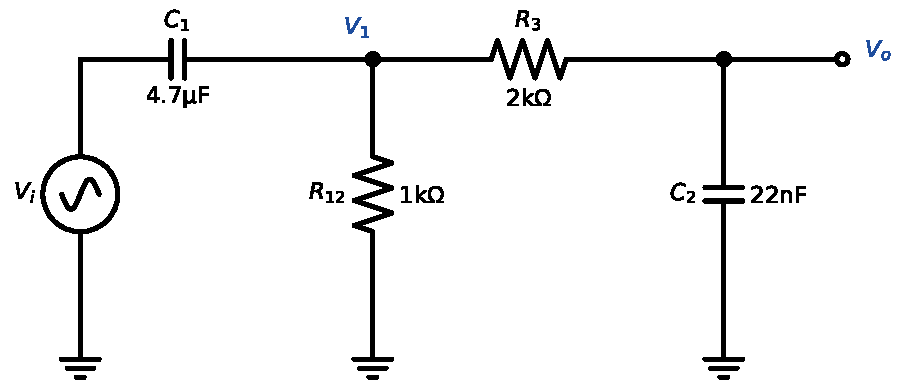
\includegraphics[width=0.95\linewidth,height=5.2cm,keepaspectratio]{p07_ac}\end{center}

\solstep{4}{Transfer function by a chain of dividers}Walk from the input to the output through the named nodes: $V_{i} \to V_{1} \to V_{o}$. The transfer function is the product of the node-to-node ratios (each one is a simple divider, tool T2, or a dependent source, tool T4):
\[
H(s) = \frac{V_o}{V_i} = \frac{V_{1}}{V_{i}}\cdot\frac{V_{o}}{V_{1}}
\]

Impedances seen \emph{looking right} from a node (everything from that node to ground, excluding what is on its left). Compute them from the far right toward the input:
\begin{align*}
Z_{1} &= R_{12} \parallel \left(R_{3} + \frac{1}{sC_{2}}\right) = \dfrac{667\,s + 1.52\times 10^{7}}{s + 15200}
\end{align*}

Now each link. {\small (Algebra tip: to simplify a fraction that contains fractions, multiply its top and bottom by every inner denominator; then divide top and bottom by the leading coefficient of the denominator so that it starts with a plain $s^n$.)}
\begin{align*}
\frac{V_{1}}{V_{i}} &= \frac{Z_{1}}{\frac{1}{sC_{1}} + Z_{1}} = \dfrac{s^{2} + 22700\,s}{s^{2} + 23000\,s + 4.84\times 10^{6}} \\
\frac{V_{o}}{V_{1}} &= \frac{\frac{1}{sC_{2}}}{R_{3} + \frac{1}{sC_{2}}} = \dfrac{22700}{s + 22700}
\end{align*}

Multiply the links and simplify (common factors cancel):\[
H(s) = \dfrac{22700\,s}{s^{2} + 23000\,s + 4.84\times 10^{6}}
\]

\solstep{5}{Standard (Bode-ready) form}Find the roots. Every root $s=-p$ of the denominator is a \emph{pole}, every root $s=-z$ of the numerator is a \emph{zero}; $|p|$ and $|z|$ are the corner frequencies (rad/s).
\begin{itemize}[leftmargin=*,itemsep=2pt]
\item Numerator: it has the factor $s$ $\Rightarrow$ 1 zero at $s=0$.
\item Denominator: $s^{2} + 23000\,s + 4.84\times 10^{6}$; quadratic formula:\[
s = \frac{-23000 \pm \sqrt{(23000)^2 - 4(4.84\times 10^{6})}}{2} = \frac{-23000 \pm 22600}{2} \Rightarrow s = -212,\ -22800
\]

\end{itemize}

Factored form (leading coefficient in front):
\[
H(s) = 22700\,\dfrac{s}{(s+212)(s+22800)}
\]

Bode-ready form: rewrite every $(s+p) = p\left(1+\frac{s}{p}\right)$ and $(s+z) = z\left(1+\frac{s}{z}\right)$, and collect all constants into $K$. Each $s$ in the numerator is paired with one of the \emph{lowest} poles as $\frac{s}{s+p}$ (that factor is $\approx 1$ above $p$). Then every factor except $K$ is $\approx 1$ inside the pass-band:
\[
H(s) = 0.995\,\dfrac{s}{s+2\pi\cdot 33.7}\,\dfrac{1}{1+\dfrac{s}{2\pi\cdot 3.63\mathrm{k}}},\qquad K = 0.995
\]

\begin{center}\renewcommand{\arraystretch}{1.35}
\begin{tabular}{cccc}
\toprule
type & $\omega_c$ (rad/s) & $f_c=\omega_c/2\pi$ & slope change \\
\midrule
pole & $212$ & 33.7 Hz & $-20$ dB/dec \\
pole & $22800$ & 3.63 kHz & $-20$ dB/dec \\
\bottomrule
\end{tabular}\end{center}

\solstep{6}{Magnitude Bode plot}Below every corner $|H(s)|\approx 0.0047\,s$, so the plot starts with a slope of $+20$\,dB/dec. Then, moving right, each pole bends the line down by 20\,dB/dec and each zero bends it up by 20\,dB/dec (tool T6):
\begin{center}\renewcommand{\arraystretch}{1.35}
\begin{tabular}{lcl}
\toprule
frequency range & slope & asymptote level \\
\midrule
$f<$ 33.7 Hz & $+20$ dB/dec & -0.0409 dB at end \\
33.7 Hz -- 3.63 kHz & $0$ dB/dec (flat) & -0.0409 dB at start, -0.0409 dB at end \\
$f>$ 3.63 kHz & $-20$ dB/dec & -0.0409 dB at start \\
\bottomrule
\end{tabular}\end{center}

The flat (pass-band) level is $20\log_{10}|K| = 20\log_{10}0.995 = -0.0409$\,dB.
\begin{center}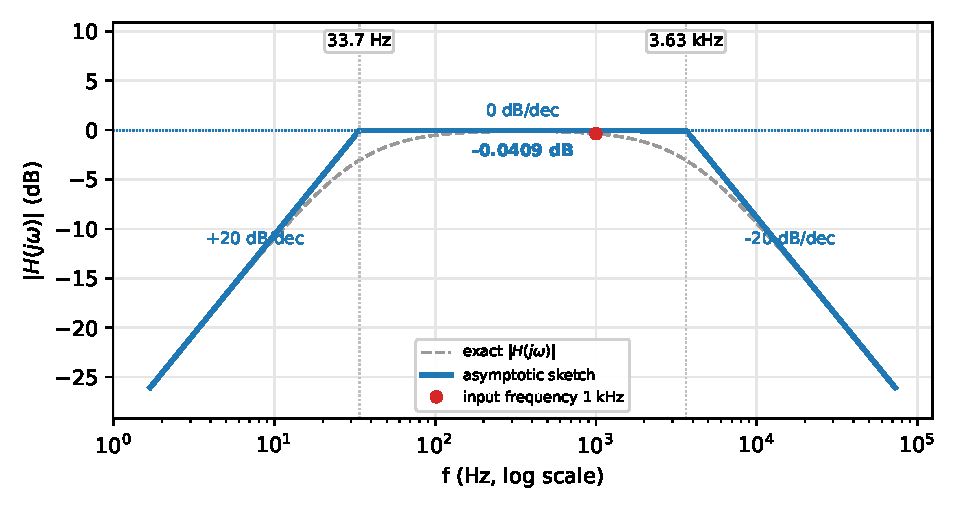
\includegraphics[width=0.78\linewidth,height=6.5cm,keepaspectratio]{p07_bode}\end{center}

{\small Blue: the straight-line sketch you are expected to draw. Dashed grey: the exact curve (about 3\,dB below the corner of an isolated pole). Red dot: the input frequency of Step 7.}
\solstep{7}{Steady-state output}The input is $V_i(t) = 0.5\sin\left(2\pi\cdot 1000\,t\right)$, so $\omega_{in} = 2\pi\cdot 1000 = 6280$\,rad/s. Put $s=j\omega_{in}$ in each factor (tool T5): magnitudes multiply, angles add.
{\small Rules: $\left|\frac{s}{s+p}\right| = \frac{\omega}{\sqrt{\omega^2+p^2}}$, $\angle = \frac{\pi}{2}-\tan^{-1}\frac{\omega}{p}$;\quad $\left|\frac{1}{1+s/p}\right| = \frac{1}{\sqrt{1+(\omega/p)^2}}$, $\angle = -\tan^{-1}\frac{\omega}{p}$;\quad $\left|1+\frac{s}{z}\right| = \sqrt{1+(\omega/z)^2}$, $\angle = \tan^{-1}\frac{\omega}{z}$;\quad a negative $K$ adds $-\pi$.}
\begin{center}\renewcommand{\arraystretch}{1.35}
\begin{tabular}{ccc}
\toprule
factor & magnitude & angle (rad) \\
\midrule
$0.995$ & $0.9953$ & $0$ \\
$\rule[-1.1em]{0pt}{2.8em}\dfrac{s}{s+2\pi\cdot 33.7}$ & $0.9994$ & $0.0337$ \\
$\rule[-1.7em]{0pt}{4em}\dfrac{1}{1+\dfrac{s}{2\pi\cdot 3.63\mathrm{k}}}$ & $0.9642$ & $-0.269$ \\
\textbf{total} & $\mathbf{0.9591}$ (product) & $\mathbf{-0.235}$ (sum) \\
\bottomrule
\end{tabular}\end{center}

\begin{align*}
|H(j\omega_{in})| &= 0.959, \qquad \angle H(j\omega_{in}) = -0.235\ \mathrm{rad} \\
v_{o,ac}(t) &= 0.959\times 0.5\,\sin\left(2\pi\cdot 1000\,t - 0.235\right) = 0.48\,\sin\left(2\pi\cdot 1000\,t - 0.235\right)
\end{align*}

Add the DC part from Step 2 (superposition):
\[
\boxed{V_o(t) = 2 + 0.48\,\sin\left(2\pi\cdot 1000\,t - 0.235\right)\ \mathrm{V}}
\]

\begin{ansbox}
$H(s) = 0.995\,\dfrac{s}{s+2\pi\cdot 33.7}\,\dfrac{1}{1+\dfrac{s}{2\pi\cdot 3.63\mathrm{k}}}$\quad (corners: 33.7 Hz, 3.63 kHz)\\[4pt]
$V_o(t) = 2 + 0.48\,\sin\left(2\pi\cdot 1000\,t - 0.235\right)\ \mathrm{V}$
\end{ansbox}

\newpage
\subsection*{Solution 1B.8 \hfill Medium}
\begin{center}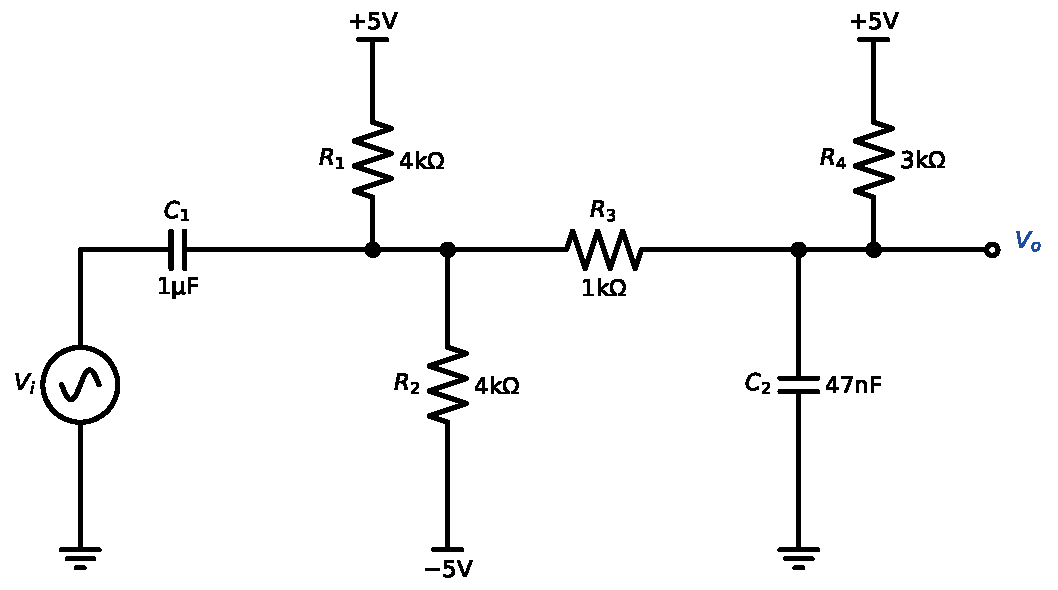
\includegraphics[width=0.8\linewidth,height=4.5cm,keepaspectratio]{p08_circuit}\end{center}
\solstep{1}{Identify the sources}Independent sources: the AC input $V_i(t)$ and the DC supplies $-5\,\mathrm{V}$, $+5\,\mathrm{V}$. Because there are both DC and AC sources, use superposition: $V_o(t) = V_{o,dc} + v_{o,ac}(t)$. Solve the DC circuit (Step 2) and the AC circuit (Steps 3--7) separately, then add.
\solstep{2}{DC circuit $\Rightarrow V_{o,dc}$}DC rules: the AC input is set to zero ($V_i=0$: a wire to ground); every capacitor is an open circuit ($C_{1}, C_{2}$). Only the part of the circuit that is still connected to $V_o$ matters:
\begin{center}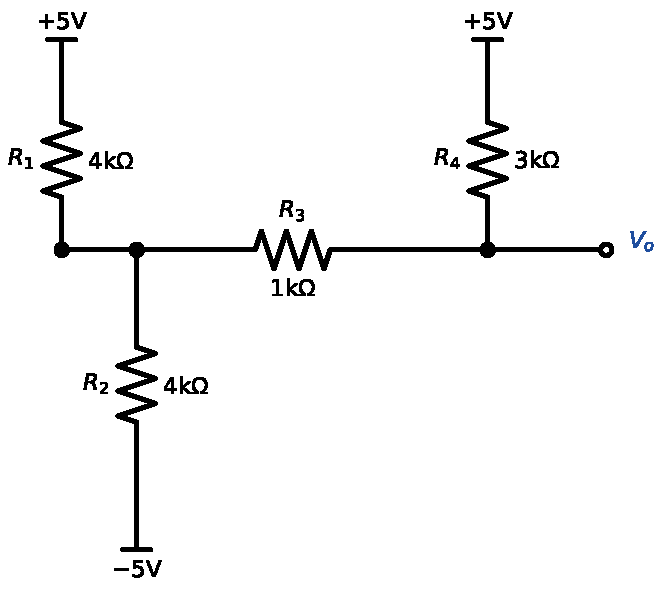
\includegraphics[width=0.55\linewidth,height=5cm,keepaspectratio]{p08_dc}\end{center}

Reduce the circuit with one tool only --- the \emph{divider between two voltages} (tool T3) --- walking toward $V_o$ and keeping a Thevenin pair $(V_{th},R_{th})$ for everything already visited.
\begin{enumerate}[leftmargin=*,itemsep=2pt]
\item Start at the input node: since $V_i=0$ it is tied to ground, i.e. it is an ideal $0\,\mathrm{V}$ source: $(V_{th},R_{th})=(0\,\mathrm{V},\,0\,\Omega)$.
\item $C_{1}$ is a capacitor $\Rightarrow$ open at DC. No DC current can cross it, so everything on its left is disconnected: start fresh after it.
\item First DC path here: $R_{1}$ to the $+5\,\mathrm{V}$ supply, so $(V_{th},R_{th}) = (5\,\mathrm{V},\ 4\,\mathrm{k}\Omega)$.
\item Add $R_{2}$ to the $-5\,\mathrm{V}$ supply. Divider between $V_a=5\,\mathrm{V}$ (through $R_a=4\,\mathrm{k}\Omega$) and $V_b=-5\,\mathrm{V}$ (through $R_b=4\,\mathrm{k}\Omega$):\[
V_{th} = V_b + (V_a-V_b)\frac{R_b}{R_a+R_b} = -5 + \left(5 - (-5)\right)\frac{4\,\mathrm{k}}{4\,\mathrm{k} + 4\,\mathrm{k}} = 0\,\mathrm{V},\qquad R_{th} = R_a\parallel R_b = 2\,\mathrm{k}\Omega
\]

\item Walk through $R_{3}$ ($1\,\mathrm{k}\Omega$ at DC). A series resistor just adds to $R_{th}$: $(V_{th},R_{th}) = (0\,\mathrm{V},\ 3\,\mathrm{k}\Omega)$.
\item Finally, collect everything at the output node $V_o$.
\item $C_{2}$ (at $V_{o}$) is a capacitor: open at DC, ignore it.
\item Add $R_{4}$ to the $+5\,\mathrm{V}$ supply. Divider between $V_a=0\,\mathrm{V}$ (through $R_a=3\,\mathrm{k}\Omega$) and $V_b=5\,\mathrm{V}$ (through $R_b=3\,\mathrm{k}\Omega$):\[
V_{th} = V_b + (V_a-V_b)\frac{R_b}{R_a+R_b} = 5 + \left(0 - (5)\right)\frac{3\,\mathrm{k}}{3\,\mathrm{k} + 3\,\mathrm{k}} = 2.5\,\mathrm{V},\qquad R_{th} = R_a\parallel R_b = 1.5\,\mathrm{k}\Omega
\]

\end{enumerate}

\[
\boxed{V_{o,dc} = 2.5\,\mathrm{V}}
\]

\solstep{3}{AC circuit}Set every DC supply to zero: each supply rail becomes AC ground. Replace every capacitor by $\frac{1}{sC}$ and every inductor by $sL$.
\begin{itemize}[leftmargin=*,itemsep=2pt]
\item $R_{1}$, $R_{2}$ both go from the same node to (AC) ground, so they are in parallel: $R_{12} = R_{1} \parallel R_{2} = 4\,\mathrm{k} \parallel 4\,\mathrm{k} = 2\,\mathrm{k}\Omega$.
\end{itemize}

AC equivalent circuit (nodes named for the next step):
\begin{center}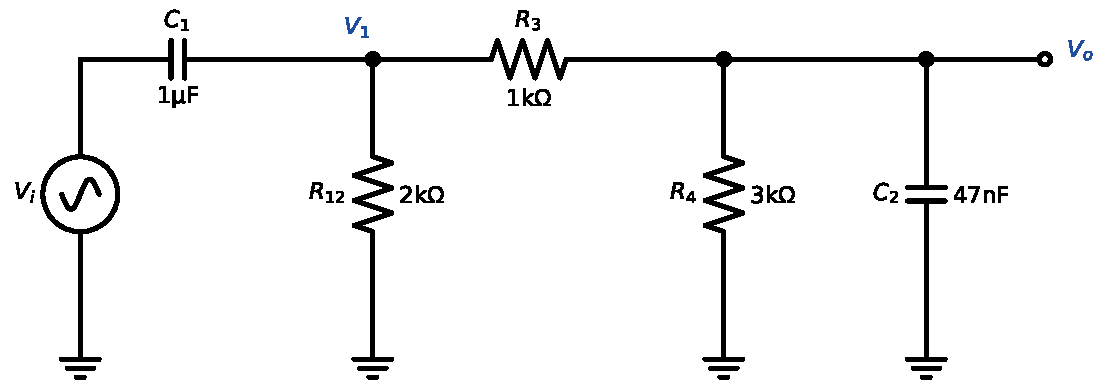
\includegraphics[width=0.95\linewidth,height=5.2cm,keepaspectratio]{p08_ac}\end{center}

\solstep{4}{Transfer function by a chain of dividers}Walk from the input to the output through the named nodes: $V_{i} \to V_{1} \to V_{o}$. The transfer function is the product of the node-to-node ratios (each one is a simple divider, tool T2, or a dependent source, tool T4):
\[
H(s) = \frac{V_o}{V_i} = \frac{V_{1}}{V_{i}}\cdot\frac{V_{o}}{V_{1}}
\]

Impedances seen \emph{looking right} from a node (everything from that node to ground, excluding what is on its left). Compute them from the far right toward the input:
\begin{align*}
Z_{o} &= R_{4} \parallel \frac{1}{sC_{2}} = \dfrac{2.13\times 10^{7}}{s + 7090} \\
Z_{1} &= R_{12} \parallel \left(R_{3} + Z_{o}\right) = \dfrac{667\,s + 1.89\times 10^{7}}{s + 14200}
\end{align*}

Now each link. {\small (Algebra tip: to simplify a fraction that contains fractions, multiply its top and bottom by every inner denominator; then divide top and bottom by the leading coefficient of the denominator so that it starts with a plain $s^n$.)}
\begin{align*}
\frac{V_{1}}{V_{i}} &= \frac{Z_{1}}{\frac{1}{sC_{1}} + Z_{1}} = \dfrac{s^{2} + 28400\,s}{s^{2} + 29900\,s + 2.13\times 10^{7}} \\
\frac{V_{o}}{V_{1}} &= \frac{Z_{o}}{R_{3} + Z_{o}} = \dfrac{21300}{s + 28400}
\end{align*}

Multiply the links and simplify (common factors cancel):\[
H(s) = \dfrac{21300\,s}{s^{2} + 29900\,s + 2.13\times 10^{7}}
\]

\solstep{5}{Standard (Bode-ready) form}Find the roots. Every root $s=-p$ of the denominator is a \emph{pole}, every root $s=-z$ of the numerator is a \emph{zero}; $|p|$ and $|z|$ are the corner frequencies (rad/s).
\begin{itemize}[leftmargin=*,itemsep=2pt]
\item Numerator: it has the factor $s$ $\Rightarrow$ 1 zero at $s=0$.
\item Denominator: $s^{2} + 29900\,s + 2.13\times 10^{7}$; quadratic formula:\[
s = \frac{-29900 \pm \sqrt{(29900)^2 - 4(2.13\times 10^{7})}}{2} = \frac{-29900 \pm 28400}{2} \Rightarrow s = -730,\ -29100
\]

\end{itemize}

Factored form (leading coefficient in front):
\[
H(s) = 21300\,\dfrac{s}{(s+730)(s+29100)}
\]

Bode-ready form: rewrite every $(s+p) = p\left(1+\frac{s}{p}\right)$ and $(s+z) = z\left(1+\frac{s}{z}\right)$, and collect all constants into $K$. Each $s$ in the numerator is paired with one of the \emph{lowest} poles as $\frac{s}{s+p}$ (that factor is $\approx 1$ above $p$). Then every factor except $K$ is $\approx 1$ inside the pass-band:
\[
H(s) = 0.73\,\dfrac{s}{s+2\pi\cdot 116}\,\dfrac{1}{1+\dfrac{s}{2\pi\cdot 4.64\mathrm{k}}},\qquad K = 0.73
\]

\begin{center}\renewcommand{\arraystretch}{1.35}
\begin{tabular}{cccc}
\toprule
type & $\omega_c$ (rad/s) & $f_c=\omega_c/2\pi$ & slope change \\
\midrule
pole & $730$ & 116 Hz & $-20$ dB/dec \\
pole & $29100$ & 4.64 kHz & $-20$ dB/dec \\
\bottomrule
\end{tabular}\end{center}

\solstep{6}{Magnitude Bode plot}Below every corner $|H(s)|\approx 0.001\,s$, so the plot starts with a slope of $+20$\,dB/dec. Then, moving right, each pole bends the line down by 20\,dB/dec and each zero bends it up by 20\,dB/dec (tool T6):
\begin{center}\renewcommand{\arraystretch}{1.35}
\begin{tabular}{lcl}
\toprule
frequency range & slope & asymptote level \\
\midrule
$f<$ 116 Hz & $+20$ dB/dec & -2.73 dB at end \\
116 Hz -- 4.64 kHz & $0$ dB/dec (flat) & -2.73 dB at start, -2.73 dB at end \\
$f>$ 4.64 kHz & $-20$ dB/dec & -2.73 dB at start \\
\bottomrule
\end{tabular}\end{center}

The flat (pass-band) level is $20\log_{10}|K| = 20\log_{10}0.73 = -2.73$\,dB.
\begin{center}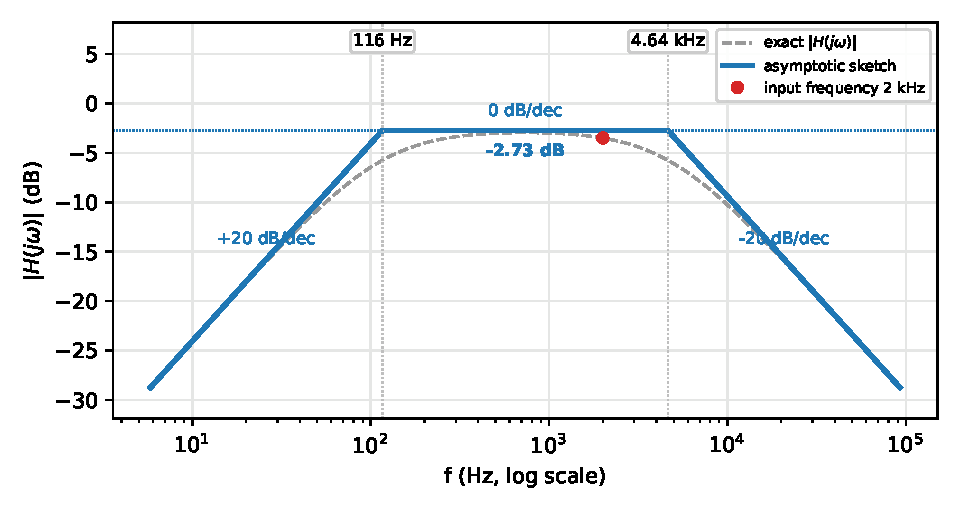
\includegraphics[width=0.78\linewidth,height=6.5cm,keepaspectratio]{p08_bode}\end{center}

{\small Blue: the straight-line sketch you are expected to draw. Dashed grey: the exact curve (about 3\,dB below the corner of an isolated pole). Red dot: the input frequency of Step 7.}
\solstep{7}{Steady-state output}The input is $V_i(t) = 0.5\sin\left(2\pi\cdot 2000\,t\right)$, so $\omega_{in} = 2\pi\cdot 2000 = 12600$\,rad/s. Put $s=j\omega_{in}$ in each factor (tool T5): magnitudes multiply, angles add.
{\small Rules: $\left|\frac{s}{s+p}\right| = \frac{\omega}{\sqrt{\omega^2+p^2}}$, $\angle = \frac{\pi}{2}-\tan^{-1}\frac{\omega}{p}$;\quad $\left|\frac{1}{1+s/p}\right| = \frac{1}{\sqrt{1+(\omega/p)^2}}$, $\angle = -\tan^{-1}\frac{\omega}{p}$;\quad $\left|1+\frac{s}{z}\right| = \sqrt{1+(\omega/z)^2}$, $\angle = \tan^{-1}\frac{\omega}{z}$;\quad a negative $K$ adds $-\pi$.}
\begin{center}\renewcommand{\arraystretch}{1.35}
\begin{tabular}{ccc}
\toprule
factor & magnitude & angle (rad) \\
\midrule
$0.73$ & $0.7302$ & $0$ \\
$\rule[-1.1em]{0pt}{2.8em}\dfrac{s}{s+2\pi\cdot 116}$ & $0.9983$ & $0.058$ \\
$\rule[-1.7em]{0pt}{4em}\dfrac{1}{1+\dfrac{s}{2\pi\cdot 4.64\mathrm{k}}}$ & $0.9182$ & $-0.407$ \\
\textbf{total} & $\mathbf{0.6694}$ (product) & $\mathbf{-0.349}$ (sum) \\
\bottomrule
\end{tabular}\end{center}

\begin{align*}
|H(j\omega_{in})| &= 0.669, \qquad \angle H(j\omega_{in}) = -0.349\ \mathrm{rad} \\
v_{o,ac}(t) &= 0.669\times 0.5\,\sin\left(2\pi\cdot 2000\,t - 0.349\right) = 0.335\,\sin\left(2\pi\cdot 2000\,t - 0.349\right)
\end{align*}

Add the DC part from Step 2 (superposition):
\[
\boxed{V_o(t) = 2.5 + 0.335\,\sin\left(2\pi\cdot 2000\,t - 0.349\right)\ \mathrm{V}}
\]

\begin{ansbox}
$H(s) = 0.73\,\dfrac{s}{s+2\pi\cdot 116}\,\dfrac{1}{1+\dfrac{s}{2\pi\cdot 4.64\mathrm{k}}}$\quad (corners: 116 Hz, 4.64 kHz)\\[4pt]
$V_o(t) = 2.5 + 0.335\,\sin\left(2\pi\cdot 2000\,t - 0.349\right)\ \mathrm{V}$
\end{ansbox}

\newpage
\subsection*{Solution 1B.9 \hfill Medium}
\begin{center}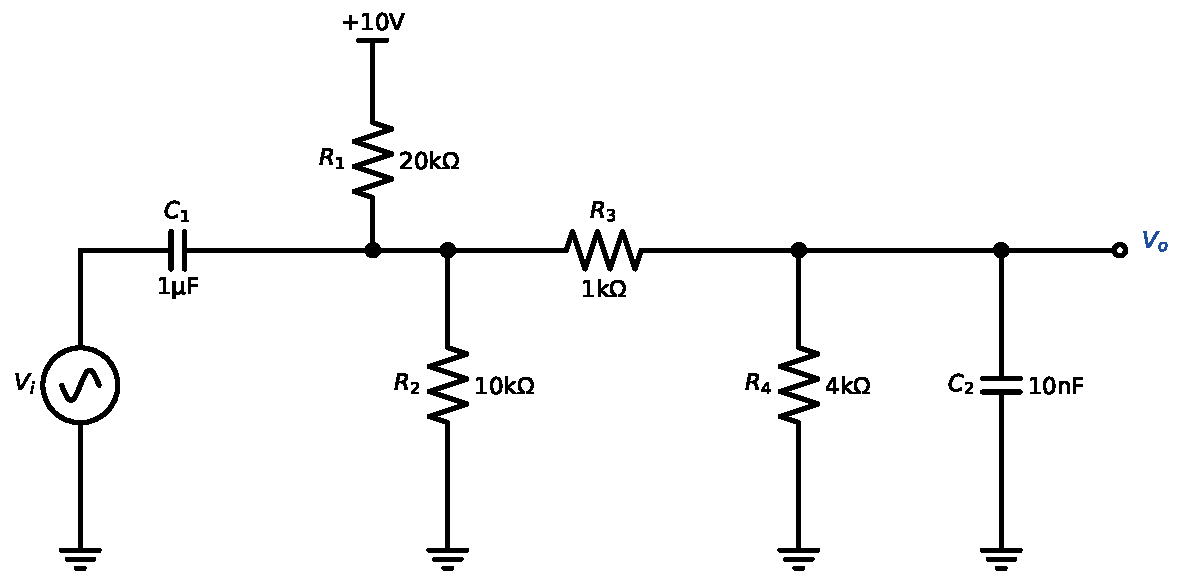
\includegraphics[width=0.8\linewidth,height=4.5cm,keepaspectratio]{p09_circuit}\end{center}
\solstep{1}{Identify the sources}Independent sources: the AC input $V_i(t)$ and the DC supplies $+10\,\mathrm{V}$. Because there are both DC and AC sources, use superposition: $V_o(t) = V_{o,dc} + v_{o,ac}(t)$. Solve the DC circuit (Step 2) and the AC circuit (Steps 3--7) separately, then add.
\solstep{2}{DC circuit $\Rightarrow V_{o,dc}$}DC rules: the AC input is set to zero ($V_i=0$: a wire to ground); every capacitor is an open circuit ($C_{1}, C_{2}$). Only the part of the circuit that is still connected to $V_o$ matters:
\begin{center}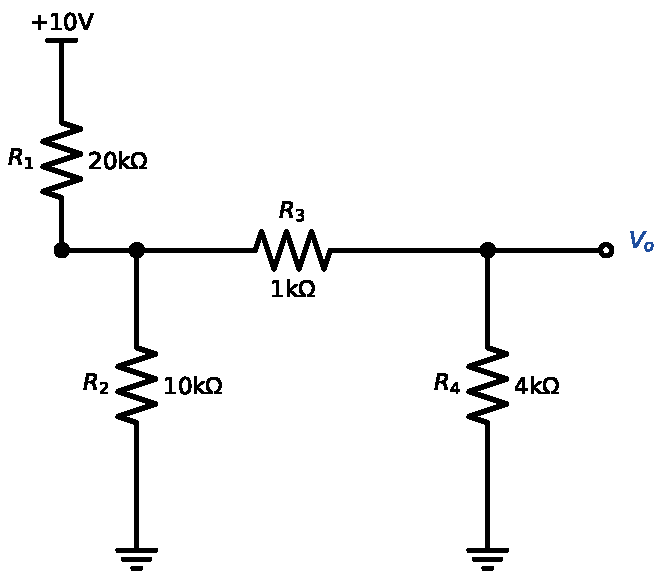
\includegraphics[width=0.55\linewidth,height=5cm,keepaspectratio]{p09_dc}\end{center}

Reduce the circuit with one tool only --- the \emph{divider between two voltages} (tool T3) --- walking toward $V_o$ and keeping a Thevenin pair $(V_{th},R_{th})$ for everything already visited.
\begin{enumerate}[leftmargin=*,itemsep=2pt]
\item Start at the input node: since $V_i=0$ it is tied to ground, i.e. it is an ideal $0\,\mathrm{V}$ source: $(V_{th},R_{th})=(0\,\mathrm{V},\,0\,\Omega)$.
\item $C_{1}$ is a capacitor $\Rightarrow$ open at DC. No DC current can cross it, so everything on its left is disconnected: start fresh after it.
\item First DC path here: $R_{1}$ to the $+10\,\mathrm{V}$ supply, so $(V_{th},R_{th}) = (10\,\mathrm{V},\ 20\,\mathrm{k}\Omega)$.
\item Add $R_{2}$ to ground. Divider between $V_a=10\,\mathrm{V}$ (through $R_a=20\,\mathrm{k}\Omega$) and $V_b=0\,\mathrm{V}$ (through $R_b=10\,\mathrm{k}\Omega$):\[
V_{th} = V_b + (V_a-V_b)\frac{R_b}{R_a+R_b} = 0 + \left(10 - (0)\right)\frac{10\,\mathrm{k}}{20\,\mathrm{k} + 10\,\mathrm{k}} = 3.33\,\mathrm{V},\qquad R_{th} = R_a\parallel R_b = 6.67\,\mathrm{k}\Omega
\]

\item Walk through $R_{3}$ ($1\,\mathrm{k}\Omega$ at DC). A series resistor just adds to $R_{th}$: $(V_{th},R_{th}) = (3.33\,\mathrm{V},\ 7.67\,\mathrm{k}\Omega)$.
\item Finally, collect everything at the output node $V_o$.
\item Add $R_{4}$ to ground. Divider between $V_a=3.33\,\mathrm{V}$ (through $R_a=7.67\,\mathrm{k}\Omega$) and $V_b=0\,\mathrm{V}$ (through $R_b=4\,\mathrm{k}\Omega$):\[
V_{th} = V_b + (V_a-V_b)\frac{R_b}{R_a+R_b} = 0 + \left(3.33 - (0)\right)\frac{4\,\mathrm{k}}{7.67\,\mathrm{k} + 4\,\mathrm{k}} = 1.14\,\mathrm{V},\qquad R_{th} = R_a\parallel R_b = 2.63\,\mathrm{k}\Omega
\]

\item $C_{2}$ (at $V_{o}$) is a capacitor: open at DC, ignore it.
\end{enumerate}

\[
\boxed{V_{o,dc} = 1.14\,\mathrm{V}}
\]

\solstep{3}{AC circuit}Set every DC supply to zero: each supply rail becomes AC ground. Replace every capacitor by $\frac{1}{sC}$ and every inductor by $sL$.
\begin{itemize}[leftmargin=*,itemsep=2pt]
\item $R_{1}$, $R_{2}$ both go from the same node to (AC) ground, so they are in parallel: $R_{12} = R_{1} \parallel R_{2} = 20\,\mathrm{k} \parallel 10\,\mathrm{k} = 6.67\,\mathrm{k}\Omega$.
\end{itemize}

AC equivalent circuit (nodes named for the next step):
\begin{center}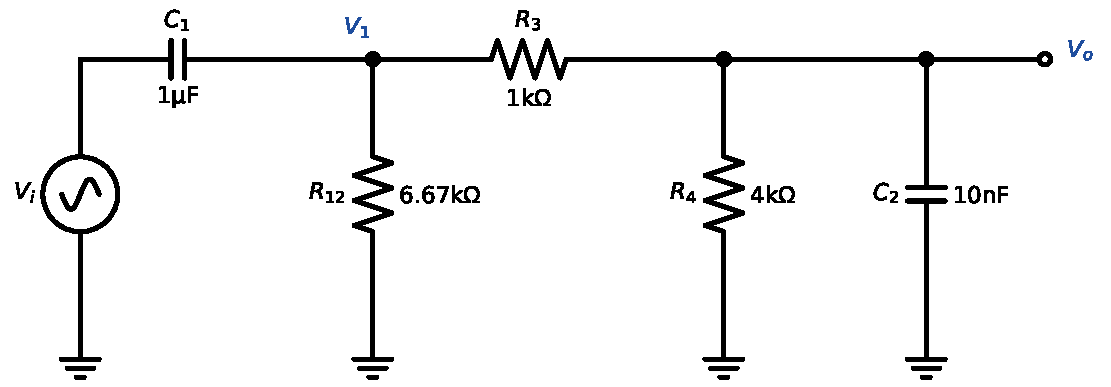
\includegraphics[width=0.95\linewidth,height=5.2cm,keepaspectratio]{p09_ac}\end{center}

\solstep{4}{Transfer function by a chain of dividers}Walk from the input to the output through the named nodes: $V_{i} \to V_{1} \to V_{o}$. The transfer function is the product of the node-to-node ratios (each one is a simple divider, tool T2, or a dependent source, tool T4):
\[
H(s) = \frac{V_o}{V_i} = \frac{V_{1}}{V_{i}}\cdot\frac{V_{o}}{V_{1}}
\]

Impedances seen \emph{looking right} from a node (everything from that node to ground, excluding what is on its left). Compute them from the far right toward the input:
\begin{align*}
Z_{o} &= R_{4} \parallel \frac{1}{sC_{2}} = \dfrac{10^{8}}{s + 25000} \\
Z_{1} &= R_{12} \parallel \left(R_{3} + Z_{o}\right) = \dfrac{870\,s + 1.09\times 10^{8}}{s + 38000}
\end{align*}

Now each link. {\small (Algebra tip: to simplify a fraction that contains fractions, multiply its top and bottom by every inner denominator; then divide top and bottom by the leading coefficient of the denominator so that it starts with a plain $s^n$.)}
\begin{align*}
\frac{V_{1}}{V_{i}} &= \frac{Z_{1}}{\frac{1}{sC_{1}} + Z_{1}} = \dfrac{s^{2} + 1.25\times 10^{5}\,s}{s^{2} + 1.26\times 10^{5}\,s + 4.38\times 10^{7}} \\
\frac{V_{o}}{V_{1}} &= \frac{Z_{o}}{R_{3} + Z_{o}} = \dfrac{10^{5}}{s + 1.25\times 10^{5}}
\end{align*}

Multiply the links and simplify (common factors cancel):\[
H(s) = \dfrac{10^{5}\,s}{s^{2} + 1.26\times 10^{5}\,s + 4.38\times 10^{7}}
\]

\solstep{5}{Standard (Bode-ready) form}Find the roots. Every root $s=-p$ of the denominator is a \emph{pole}, every root $s=-z$ of the numerator is a \emph{zero}; $|p|$ and $|z|$ are the corner frequencies (rad/s).
\begin{itemize}[leftmargin=*,itemsep=2pt]
\item Numerator: it has the factor $s$ $\Rightarrow$ 1 zero at $s=0$.
\item Denominator: $s^{2} + 1.26\times 10^{5}\,s + 4.38\times 10^{7}$; quadratic formula:\[
s = \frac{-1.26\times 10^{5} \pm \sqrt{(1.26\times 10^{5})^2 - 4(4.38\times 10^{7})}}{2} = \frac{-1.26\times 10^{5} \pm 1.25\times 10^{5}}{2} \Rightarrow s = -348,\ -1.26\times 10^{5}
\]

\end{itemize}

Factored form (leading coefficient in front):
\[
H(s) = 10^{5}\,\dfrac{s}{(s+348)(s+1.26\times 10^{5})}
\]

Bode-ready form: rewrite every $(s+p) = p\left(1+\frac{s}{p}\right)$ and $(s+z) = z\left(1+\frac{s}{z}\right)$, and collect all constants into $K$. Each $s$ in the numerator is paired with one of the \emph{lowest} poles as $\frac{s}{s+p}$ (that factor is $\approx 1$ above $p$). Then every factor except $K$ is $\approx 1$ inside the pass-band:
\[
H(s) = 0.795\,\dfrac{s}{s+2\pi\cdot 55.3}\,\dfrac{1}{1+\dfrac{s}{2\pi\cdot 20\mathrm{k}}},\qquad K = 0.795
\]

\begin{center}\renewcommand{\arraystretch}{1.35}
\begin{tabular}{cccc}
\toprule
type & $\omega_c$ (rad/s) & $f_c=\omega_c/2\pi$ & slope change \\
\midrule
pole & $348$ & 55.3 Hz & $-20$ dB/dec \\
pole & $1.26\times 10^{5}$ & 20 kHz & $-20$ dB/dec \\
\bottomrule
\end{tabular}\end{center}

\solstep{6}{Magnitude Bode plot}Below every corner $|H(s)|\approx 0.00229\,s$, so the plot starts with a slope of $+20$\,dB/dec. Then, moving right, each pole bends the line down by 20\,dB/dec and each zero bends it up by 20\,dB/dec (tool T6):
\begin{center}\renewcommand{\arraystretch}{1.35}
\begin{tabular}{lcl}
\toprule
frequency range & slope & asymptote level \\
\midrule
$f<$ 55.3 Hz & $+20$ dB/dec & -1.99 dB at end \\
55.3 Hz -- 20 kHz & $0$ dB/dec (flat) & -1.99 dB at start, -1.99 dB at end \\
$f>$ 20 kHz & $-20$ dB/dec & -1.99 dB at start \\
\bottomrule
\end{tabular}\end{center}

The flat (pass-band) level is $20\log_{10}|K| = 20\log_{10}0.795 = -1.99$\,dB.
\begin{center}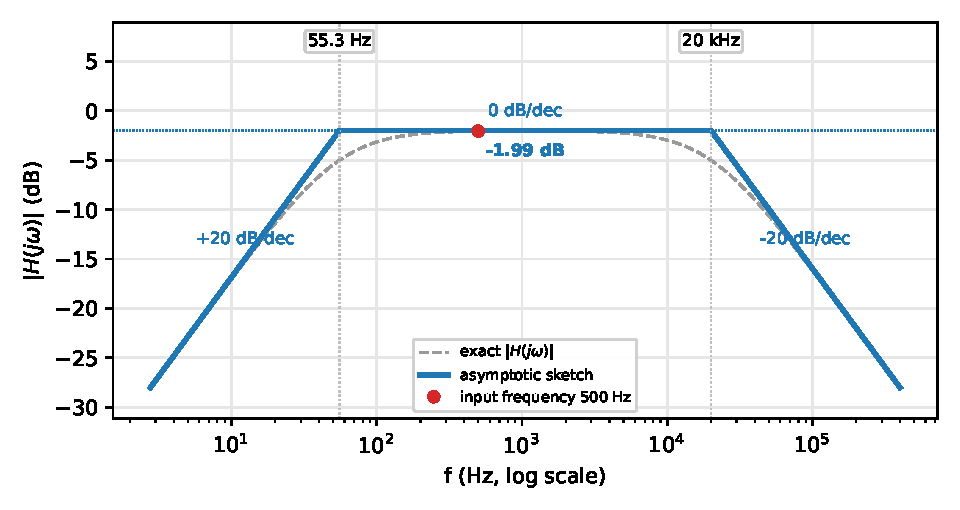
\includegraphics[width=0.78\linewidth,height=6.5cm,keepaspectratio]{p09_bode}\end{center}

{\small Blue: the straight-line sketch you are expected to draw. Dashed grey: the exact curve (about 3\,dB below the corner of an isolated pole). Red dot: the input frequency of Step 7.}
\solstep{7}{Steady-state output}The input is $V_i(t) = 1\sin\left(2\pi\cdot 500\,t\right)$, so $\omega_{in} = 2\pi\cdot 500 = 3140$\,rad/s. Put $s=j\omega_{in}$ in each factor (tool T5): magnitudes multiply, angles add.
{\small Rules: $\left|\frac{s}{s+p}\right| = \frac{\omega}{\sqrt{\omega^2+p^2}}$, $\angle = \frac{\pi}{2}-\tan^{-1}\frac{\omega}{p}$;\quad $\left|\frac{1}{1+s/p}\right| = \frac{1}{\sqrt{1+(\omega/p)^2}}$, $\angle = -\tan^{-1}\frac{\omega}{p}$;\quad $\left|1+\frac{s}{z}\right| = \sqrt{1+(\omega/z)^2}$, $\angle = \tan^{-1}\frac{\omega}{z}$;\quad a negative $K$ adds $-\pi$.}
\begin{center}\renewcommand{\arraystretch}{1.35}
\begin{tabular}{ccc}
\toprule
factor & magnitude & angle (rad) \\
\midrule
$0.795$ & $0.7949$ & $0$ \\
$\rule[-1.1em]{0pt}{2.8em}\dfrac{s}{s+2\pi\cdot 55.3}$ & $0.9939$ & $0.11$ \\
$\rule[-1.7em]{0pt}{4em}\dfrac{1}{1+\dfrac{s}{2\pi\cdot 20\mathrm{k}}}$ & $0.9997$ & $-0.025$ \\
\textbf{total} & $\mathbf{0.7898}$ (product) & $\mathbf{0.0853}$ (sum) \\
\bottomrule
\end{tabular}\end{center}

\begin{align*}
|H(j\omega_{in})| &= 0.79, \qquad \angle H(j\omega_{in}) = 0.0853\ \mathrm{rad} \\
v_{o,ac}(t) &= 0.79\times 1\,\sin\left(2\pi\cdot 500\,t + 0.0853\right) = 0.79\,\sin\left(2\pi\cdot 500\,t + 0.0853\right)
\end{align*}

Add the DC part from Step 2 (superposition):
\[
\boxed{V_o(t) = 1.14 + 0.79\,\sin\left(2\pi\cdot 500\,t + 0.0853\right)\ \mathrm{V}}
\]

\begin{ansbox}
$H(s) = 0.795\,\dfrac{s}{s+2\pi\cdot 55.3}\,\dfrac{1}{1+\dfrac{s}{2\pi\cdot 20\mathrm{k}}}$\quad (corners: 55.3 Hz, 20 kHz)\\[4pt]
$V_o(t) = 1.14 + 0.79\,\sin\left(2\pi\cdot 500\,t + 0.0853\right)\ \mathrm{V}$
\end{ansbox}

\newpage
\subsection*{Solution 1B.10 \hfill Medium}
\begin{center}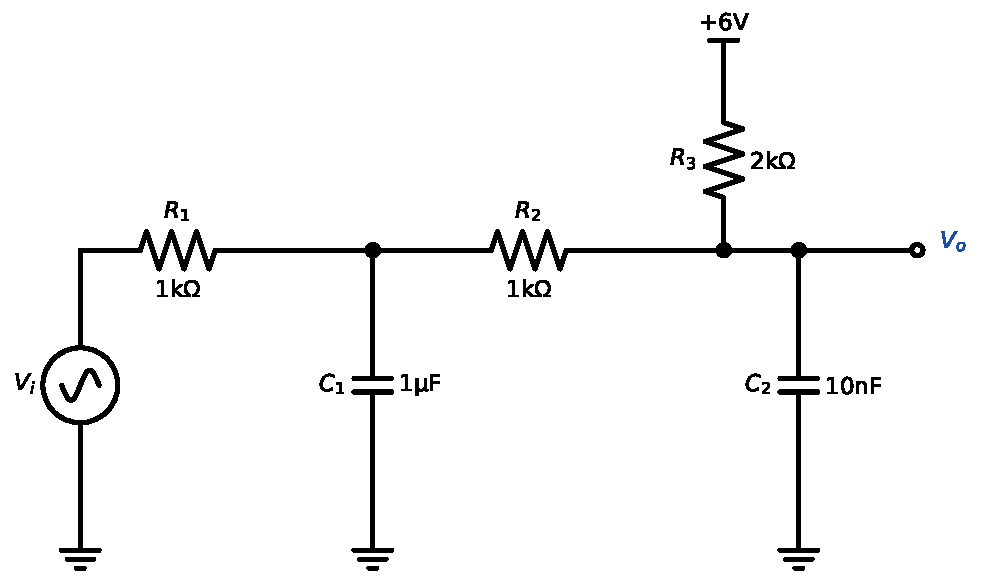
\includegraphics[width=0.8\linewidth,height=4.5cm,keepaspectratio]{p10_circuit}\end{center}
\solstep{1}{Identify the sources}Independent sources: the AC input $V_i(t)$ and the DC supplies $+6\,\mathrm{V}$. Because there are both DC and AC sources, use superposition: $V_o(t) = V_{o,dc} + v_{o,ac}(t)$. Solve the DC circuit (Step 2) and the AC circuit (Steps 3--7) separately, then add.
\solstep{2}{DC circuit $\Rightarrow V_{o,dc}$}DC rules: the AC input is set to zero ($V_i=0$: a wire to ground); every capacitor is an open circuit ($C_{1}, C_{2}$). Only the part of the circuit that is still connected to $V_o$ matters:
\begin{center}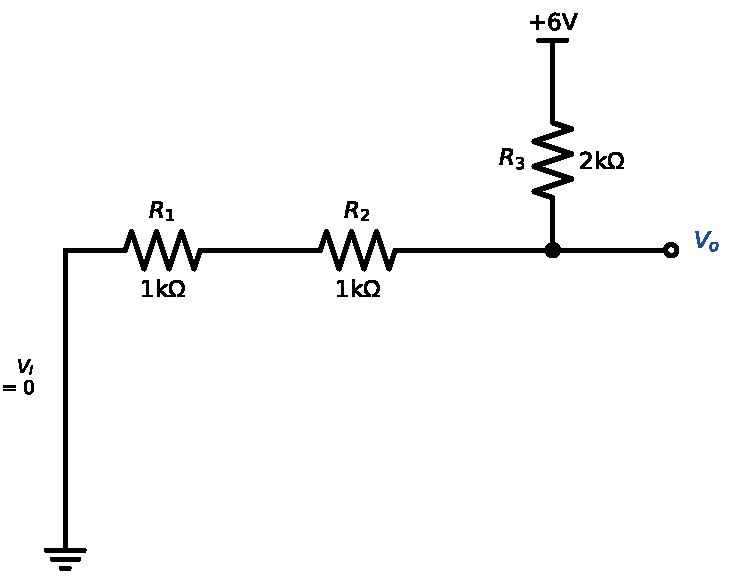
\includegraphics[width=0.55\linewidth,height=5cm,keepaspectratio]{p10_dc}\end{center}

Reduce the circuit with one tool only --- the \emph{divider between two voltages} (tool T3) --- walking toward $V_o$ and keeping a Thevenin pair $(V_{th},R_{th})$ for everything already visited.
\begin{enumerate}[leftmargin=*,itemsep=2pt]
\item Start at the input node: since $V_i=0$ it is tied to ground, i.e. it is an ideal $0\,\mathrm{V}$ source: $(V_{th},R_{th})=(0\,\mathrm{V},\,0\,\Omega)$.
\item Walk through $R_{1}$ ($1\,\mathrm{k}\Omega$ at DC). A series resistor just adds to $R_{th}$: $(V_{th},R_{th}) = (0\,\mathrm{V},\ 1\,\mathrm{k}\Omega)$.
\item $C_{1}$ (at $V_{1}$) is a capacitor: open at DC, ignore it.
\item Walk through $R_{2}$ ($1\,\mathrm{k}\Omega$ at DC). A series resistor just adds to $R_{th}$: $(V_{th},R_{th}) = (0\,\mathrm{V},\ 2\,\mathrm{k}\Omega)$.
\item Finally, collect everything at the output node $V_o$.
\item Add $R_{3}$ to the $+6\,\mathrm{V}$ supply. Divider between $V_a=0\,\mathrm{V}$ (through $R_a=2\,\mathrm{k}\Omega$) and $V_b=6\,\mathrm{V}$ (through $R_b=2\,\mathrm{k}\Omega$):\[
V_{th} = V_b + (V_a-V_b)\frac{R_b}{R_a+R_b} = 6 + \left(0 - (6)\right)\frac{2\,\mathrm{k}}{2\,\mathrm{k} + 2\,\mathrm{k}} = 3\,\mathrm{V},\qquad R_{th} = R_a\parallel R_b = 1\,\mathrm{k}\Omega
\]

\item $C_{2}$ (at $V_{o}$) is a capacitor: open at DC, ignore it.
\end{enumerate}

\[
\boxed{V_{o,dc} = 3\,\mathrm{V}}
\]

\solstep{3}{AC circuit}Set every DC supply to zero: each supply rail becomes AC ground. Replace every capacitor by $\frac{1}{sC}$ and every inductor by $sL$.
AC equivalent circuit (nodes named for the next step):
\begin{center}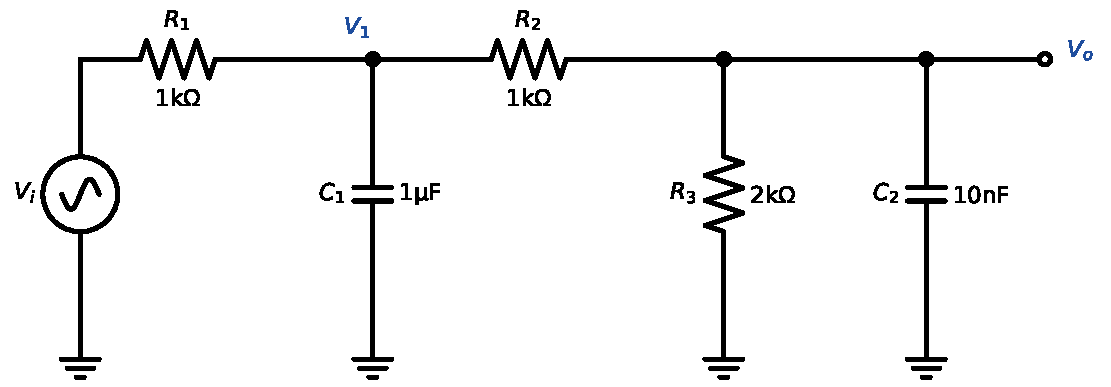
\includegraphics[width=0.95\linewidth,height=5.2cm,keepaspectratio]{p10_ac}\end{center}

\solstep{4}{Transfer function by a chain of dividers}Walk from the input to the output through the named nodes: $V_{i} \to V_{1} \to V_{o}$. The transfer function is the product of the node-to-node ratios (each one is a simple divider, tool T2, or a dependent source, tool T4):
\[
H(s) = \frac{V_o}{V_i} = \frac{V_{1}}{V_{i}}\cdot\frac{V_{o}}{V_{1}}
\]

Impedances seen \emph{looking right} from a node (everything from that node to ground, excluding what is on its left). Compute them from the far right toward the input:
\begin{align*}
Z_{o} &= R_{3} \parallel \frac{1}{sC_{2}} = \dfrac{10^{8}}{s + 50000} \\
Z_{1} &= \frac{1}{sC_{1}} \parallel \left(R_{2} + Z_{o}\right) = \dfrac{10^{6}\,s + 1.5\times 10^{11}}{s^{2} + 1.51\times 10^{5}\,s + 5\times 10^{7}}
\end{align*}

Now each link. {\small (Algebra tip: to simplify a fraction that contains fractions, multiply its top and bottom by every inner denominator; then divide top and bottom by the leading coefficient of the denominator so that it starts with a plain $s^n$.)}
\begin{align*}
\frac{V_{1}}{V_{i}} &= \frac{Z_{1}}{R_{1} + Z_{1}} = \dfrac{1000\,s + 1.5\times 10^{8}}{s^{2} + 1.52\times 10^{5}\,s + 2\times 10^{8}} \\
\frac{V_{o}}{V_{1}} &= \frac{Z_{o}}{R_{2} + Z_{o}} = \dfrac{10^{5}}{s + 1.5\times 10^{5}}
\end{align*}

Multiply the links and simplify (common factors cancel):\[
H(s) = \dfrac{10^{8}}{s^{2} + 1.52\times 10^{5}\,s + 2\times 10^{8}}
\]

\solstep{5}{Standard (Bode-ready) form}Find the roots. Every root $s=-p$ of the denominator is a \emph{pole}, every root $s=-z$ of the numerator is a \emph{zero}; $|p|$ and $|z|$ are the corner frequencies (rad/s).
\begin{itemize}[leftmargin=*,itemsep=2pt]
\item Denominator: $s^{2} + 1.52\times 10^{5}\,s + 2\times 10^{8}$; quadratic formula:\[
s = \frac{-1.52\times 10^{5} \pm \sqrt{(1.52\times 10^{5})^2 - 4(2\times 10^{8})}}{2} = \frac{-1.52\times 10^{5} \pm 1.49\times 10^{5}}{2} \Rightarrow s = -1330,\ -1.51\times 10^{5}
\]

\end{itemize}

Factored form (leading coefficient in front):
\[
H(s) = 10^{8}\,\dfrac{1}{(s+1330)(s+1.51\times 10^{5})}
\]

Bode-ready form: rewrite every $(s+p) = p\left(1+\frac{s}{p}\right)$ and $(s+z) = z\left(1+\frac{s}{z}\right)$, and collect all constants into $K$. Then every factor except $K$ is $\approx 1$ inside the pass-band:
\[
H(s) = 0.5\,\dfrac{1}{1+\dfrac{s}{2\pi\cdot 211}}\,\dfrac{1}{1+\dfrac{s}{2\pi\cdot 24\mathrm{k}}},\qquad K = 0.5
\]

\begin{center}\renewcommand{\arraystretch}{1.35}
\begin{tabular}{cccc}
\toprule
type & $\omega_c$ (rad/s) & $f_c=\omega_c/2\pi$ & slope change \\
\midrule
pole & $1330$ & 211 Hz & $-20$ dB/dec \\
pole & $1.51\times 10^{5}$ & 24 kHz & $-20$ dB/dec \\
\bottomrule
\end{tabular}\end{center}

\solstep{6}{Magnitude Bode plot}Below every corner, all factors are $\approx$ constant: $|H| \approx 0.5$ $= -6.02$\,dB (flat, 0 dB/dec). Then, moving right, each pole bends the line down by 20\,dB/dec and each zero bends it up by 20\,dB/dec (tool T6):
\begin{center}\renewcommand{\arraystretch}{1.35}
\begin{tabular}{lcl}
\toprule
frequency range & slope & asymptote level \\
\midrule
$f<$ 211 Hz & $0$ dB/dec (flat) & -6.02 dB at end \\
211 Hz -- 24 kHz & $-20$ dB/dec & -6.02 dB at start, -47.1 dB at end \\
$f>$ 24 kHz & $-40$ dB/dec & -47.1 dB at start \\
\bottomrule
\end{tabular}\end{center}

The flat (pass-band) level is $20\log_{10}|K| = 20\log_{10}0.5 = -6.02$\,dB.
\begin{center}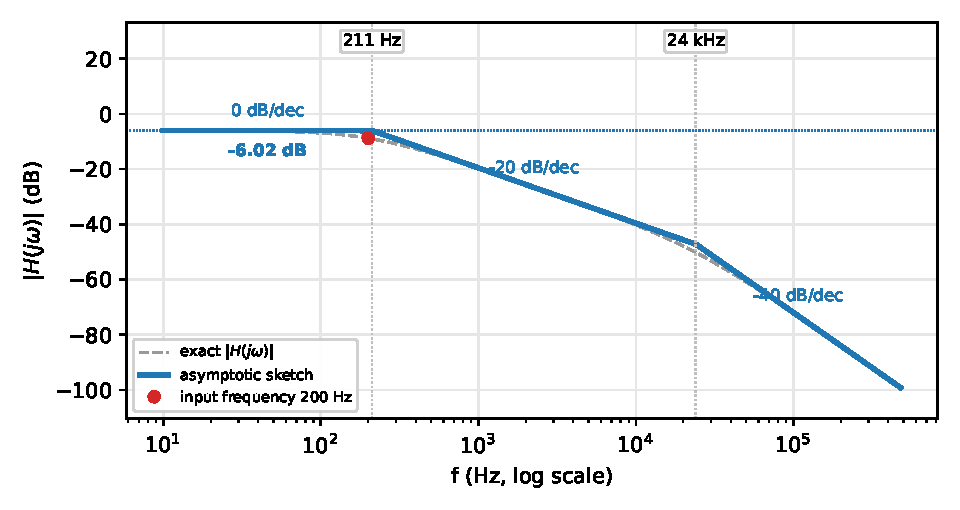
\includegraphics[width=0.78\linewidth,height=6.5cm,keepaspectratio]{p10_bode}\end{center}

{\small Blue: the straight-line sketch you are expected to draw. Dashed grey: the exact curve (about 3\,dB below the corner of an isolated pole). Red dot: the input frequency of Step 7.}
\solstep{7}{Steady-state output}The input is $V_i(t) = 1\sin\left(2\pi\cdot 200\,t\right)$, so $\omega_{in} = 2\pi\cdot 200 = 1260$\,rad/s. Put $s=j\omega_{in}$ in each factor (tool T5): magnitudes multiply, angles add.
{\small Rules: $\left|\frac{s}{s+p}\right| = \frac{\omega}{\sqrt{\omega^2+p^2}}$, $\angle = \frac{\pi}{2}-\tan^{-1}\frac{\omega}{p}$;\quad $\left|\frac{1}{1+s/p}\right| = \frac{1}{\sqrt{1+(\omega/p)^2}}$, $\angle = -\tan^{-1}\frac{\omega}{p}$;\quad $\left|1+\frac{s}{z}\right| = \sqrt{1+(\omega/z)^2}$, $\angle = \tan^{-1}\frac{\omega}{z}$;\quad a negative $K$ adds $-\pi$.}
\begin{center}\renewcommand{\arraystretch}{1.35}
\begin{tabular}{ccc}
\toprule
factor & magnitude & angle (rad) \\
\midrule
$0.5$ & $0.5$ & $0$ \\
$\rule[-1.7em]{0pt}{4em}\dfrac{1}{1+\dfrac{s}{2\pi\cdot 211}}$ & $0.7262$ & $-0.758$ \\
$\rule[-1.7em]{0pt}{4em}\dfrac{1}{1+\dfrac{s}{2\pi\cdot 24\mathrm{k}}}$ & $1$ & $-0.00834$ \\
\textbf{total} & $\mathbf{0.3631}$ (product) & $\mathbf{-0.766}$ (sum) \\
\bottomrule
\end{tabular}\end{center}

\begin{align*}
|H(j\omega_{in})| &= 0.363, \qquad \angle H(j\omega_{in}) = -0.766\ \mathrm{rad} \\
v_{o,ac}(t) &= 0.363\times 1\,\sin\left(2\pi\cdot 200\,t - 0.766\right) = 0.363\,\sin\left(2\pi\cdot 200\,t - 0.766\right)
\end{align*}

Add the DC part from Step 2 (superposition):
\[
\boxed{V_o(t) = 3 + 0.363\,\sin\left(2\pi\cdot 200\,t - 0.766\right)\ \mathrm{V}}
\]

\begin{ansbox}
$H(s) = 0.5\,\dfrac{1}{1+\dfrac{s}{2\pi\cdot 211}}\,\dfrac{1}{1+\dfrac{s}{2\pi\cdot 24\mathrm{k}}}$\quad (corners: 211 Hz, 24 kHz)\\[4pt]
$V_o(t) = 3 + 0.363\,\sin\left(2\pi\cdot 200\,t - 0.766\right)\ \mathrm{V}$
\end{ansbox}

\newpage
\subsection*{Solution 1B.11 \hfill Medium}
\begin{center}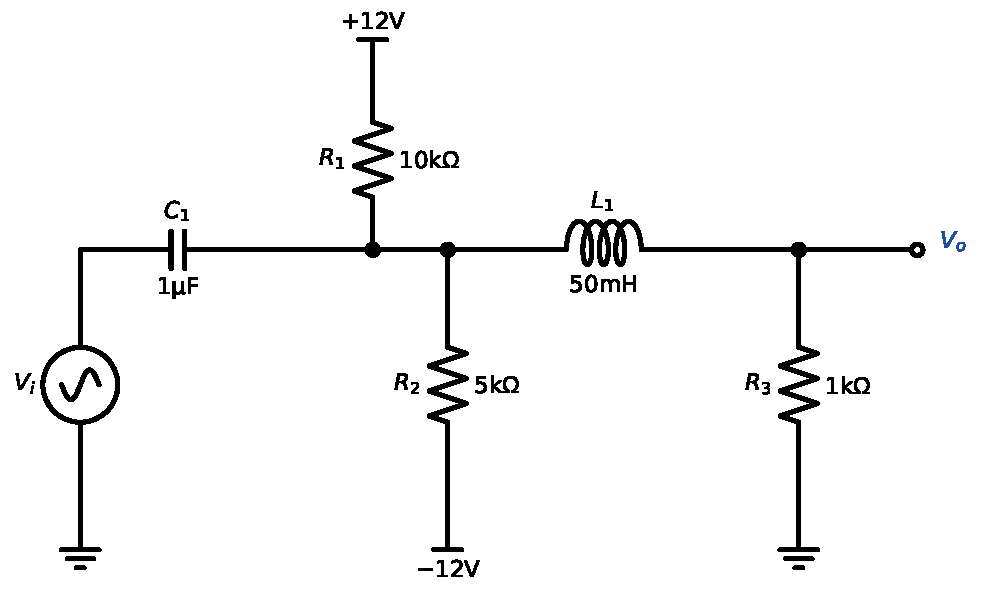
\includegraphics[width=0.8\linewidth,height=4.5cm,keepaspectratio]{p11_circuit}\end{center}
\solstep{1}{Identify the sources}Independent sources: the AC input $V_i(t)$ and the DC supplies $-12\,\mathrm{V}$, $+12\,\mathrm{V}$. Because there are both DC and AC sources, use superposition: $V_o(t) = V_{o,dc} + v_{o,ac}(t)$. Solve the DC circuit (Step 2) and the AC circuit (Steps 3--7) separately, then add.
\solstep{2}{DC circuit $\Rightarrow V_{o,dc}$}DC rules: the AC input is set to zero ($V_i=0$: a wire to ground); every capacitor is an open circuit ($C_{1}$); every inductor is a short circuit ($L_{1}$). Only the part of the circuit that is still connected to $V_o$ matters:
\begin{center}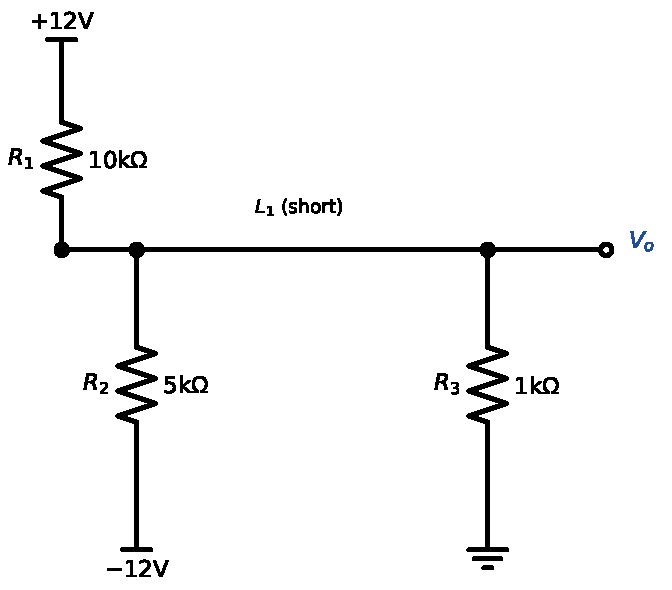
\includegraphics[width=0.55\linewidth,height=5cm,keepaspectratio]{p11_dc}\end{center}

Reduce the circuit with one tool only --- the \emph{divider between two voltages} (tool T3) --- walking toward $V_o$ and keeping a Thevenin pair $(V_{th},R_{th})$ for everything already visited.
\begin{enumerate}[leftmargin=*,itemsep=2pt]
\item Start at the input node: since $V_i=0$ it is tied to ground, i.e. it is an ideal $0\,\mathrm{V}$ source: $(V_{th},R_{th})=(0\,\mathrm{V},\,0\,\Omega)$.
\item $C_{1}$ is a capacitor $\Rightarrow$ open at DC. No DC current can cross it, so everything on its left is disconnected: start fresh after it.
\item First DC path here: $R_{1}$ to the $+12\,\mathrm{V}$ supply, so $(V_{th},R_{th}) = (12\,\mathrm{V},\ 10\,\mathrm{k}\Omega)$.
\item Add $R_{2}$ to the $-12\,\mathrm{V}$ supply. Divider between $V_a=12\,\mathrm{V}$ (through $R_a=10\,\mathrm{k}\Omega$) and $V_b=-12\,\mathrm{V}$ (through $R_b=5\,\mathrm{k}\Omega$):\[
V_{th} = V_b + (V_a-V_b)\frac{R_b}{R_a+R_b} = -12 + \left(12 - (-12)\right)\frac{5\,\mathrm{k}}{10\,\mathrm{k} + 5\,\mathrm{k}} = -4\,\mathrm{V},\qquad R_{th} = R_a\parallel R_b = 3.33\,\mathrm{k}\Omega
\]

\item $L_{1}$ is a short at DC (inductor), so the pair is unchanged.
\item Finally, collect everything at the output node $V_o$.
\item Add $R_{3}$ to ground. Divider between $V_a=-4\,\mathrm{V}$ (through $R_a=3.33\,\mathrm{k}\Omega$) and $V_b=0\,\mathrm{V}$ (through $R_b=1\,\mathrm{k}\Omega$):\[
V_{th} = V_b + (V_a-V_b)\frac{R_b}{R_a+R_b} = 0 + \left(-4 - (0)\right)\frac{1\,\mathrm{k}}{3.33\,\mathrm{k} + 1\,\mathrm{k}} = -923\,\mathrm{m}\mathrm{V},\qquad R_{th} = R_a\parallel R_b = 769\,\Omega
\]

\end{enumerate}

\[
\boxed{V_{o,dc} = -923\,\mathrm{m}\mathrm{V}}
\]

\solstep{3}{AC circuit}Set every DC supply to zero: each supply rail becomes AC ground. Replace every capacitor by $\frac{1}{sC}$ and every inductor by $sL$.
\begin{itemize}[leftmargin=*,itemsep=2pt]
\item $R_{1}$, $R_{2}$ both go from the same node to (AC) ground, so they are in parallel: $R_{12} = R_{1} \parallel R_{2} = 10\,\mathrm{k} \parallel 5\,\mathrm{k} = 3.33\,\mathrm{k}\Omega$.
\end{itemize}

AC equivalent circuit (nodes named for the next step):
\begin{center}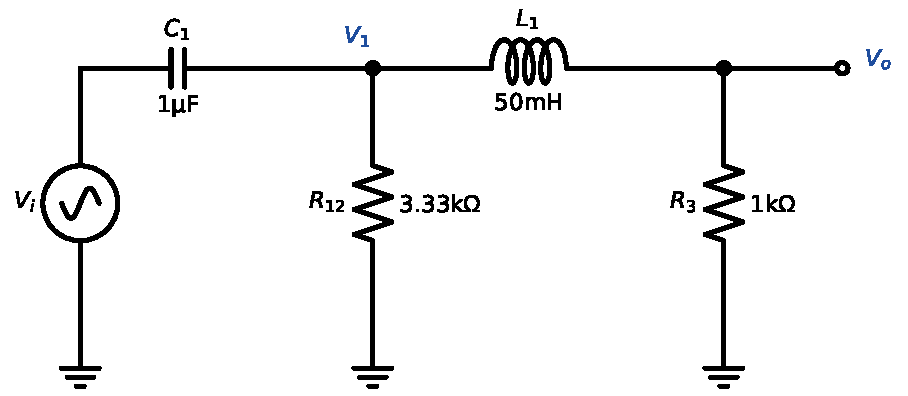
\includegraphics[width=0.95\linewidth,height=5.2cm,keepaspectratio]{p11_ac}\end{center}

\solstep{4}{Transfer function by a chain of dividers}Walk from the input to the output through the named nodes: $V_{i} \to V_{1} \to V_{o}$. The transfer function is the product of the node-to-node ratios (each one is a simple divider, tool T2, or a dependent source, tool T4):
\[
H(s) = \frac{V_o}{V_i} = \frac{V_{1}}{V_{i}}\cdot\frac{V_{o}}{V_{1}}
\]

Impedances seen \emph{looking right} from a node (everything from that node to ground, excluding what is on its left). Compute them from the far right toward the input:
\begin{align*}
Z_{1} &= R_{12} \parallel \left(sL_{1} + R_{3}\right) = \dfrac{3330\,s + 6.67\times 10^{7}}{s + 86700}
\end{align*}

Now each link. {\small (Algebra tip: to simplify a fraction that contains fractions, multiply its top and bottom by every inner denominator; then divide top and bottom by the leading coefficient of the denominator so that it starts with a plain $s^n$.)}
\begin{align*}
\frac{V_{1}}{V_{i}} &= \frac{Z_{1}}{\frac{1}{sC_{1}} + Z_{1}} = \dfrac{s^{2} + 20000\,s}{s^{2} + 20300\,s + 2.6\times 10^{7}} \\
\frac{V_{o}}{V_{1}} &= \frac{R_{3}}{sL_{1} + R_{3}} = \dfrac{20000}{s + 20000}
\end{align*}

Multiply the links and simplify (common factors cancel):\[
H(s) = \dfrac{20000\,s}{s^{2} + 20300\,s + 2.6\times 10^{7}}
\]

\solstep{5}{Standard (Bode-ready) form}Find the roots. Every root $s=-p$ of the denominator is a \emph{pole}, every root $s=-z$ of the numerator is a \emph{zero}; $|p|$ and $|z|$ are the corner frequencies (rad/s).
\begin{itemize}[leftmargin=*,itemsep=2pt]
\item Numerator: it has the factor $s$ $\Rightarrow$ 1 zero at $s=0$.
\item Denominator: $s^{2} + 20300\,s + 2.6\times 10^{7}$; quadratic formula:\[
s = \frac{-20300 \pm \sqrt{(20300)^2 - 4(2.6\times 10^{7})}}{2} = \frac{-20300 \pm 17600}{2} \Rightarrow s = -1370,\ -18900
\]

\end{itemize}

Factored form (leading coefficient in front):
\[
H(s) = 20000\,\dfrac{s}{(s+1370)(s+18900)}
\]

Bode-ready form: rewrite every $(s+p) = p\left(1+\frac{s}{p}\right)$ and $(s+z) = z\left(1+\frac{s}{z}\right)$, and collect all constants into $K$. Each $s$ in the numerator is paired with one of the \emph{lowest} poles as $\frac{s}{s+p}$ (that factor is $\approx 1$ above $p$). Then every factor except $K$ is $\approx 1$ inside the pass-band:
\[
H(s) = 1.06\,\dfrac{s}{s+2\pi\cdot 219}\,\dfrac{1}{1+\dfrac{s}{2\pi\cdot 3.01\mathrm{k}}},\qquad K = 1.06
\]

\begin{center}\renewcommand{\arraystretch}{1.35}
\begin{tabular}{cccc}
\toprule
type & $\omega_c$ (rad/s) & $f_c=\omega_c/2\pi$ & slope change \\
\midrule
pole & $1370$ & 219 Hz & $-20$ dB/dec \\
pole & $18900$ & 3.01 kHz & $-20$ dB/dec \\
\bottomrule
\end{tabular}\end{center}

\solstep{6}{Magnitude Bode plot}Below every corner $|H(s)|\approx 7.69\times 10^{-4}\,s$, so the plot starts with a slope of $+20$\,dB/dec. Then, moving right, each pole bends the line down by 20\,dB/dec and each zero bends it up by 20\,dB/dec (tool T6):
\begin{center}\renewcommand{\arraystretch}{1.35}
\begin{tabular}{lcl}
\toprule
frequency range & slope & asymptote level \\
\midrule
$f<$ 219 Hz & $+20$ dB/dec & 0.479 dB at end \\
219 Hz -- 3.01 kHz & $0$ dB/dec (flat) & 0.479 dB at start, 0.479 dB at end \\
$f>$ 3.01 kHz & $-20$ dB/dec & 0.479 dB at start \\
\bottomrule
\end{tabular}\end{center}

The flat (pass-band) level is $20\log_{10}|K| = 20\log_{10}1.06 = 0.479$\,dB.
\begin{center}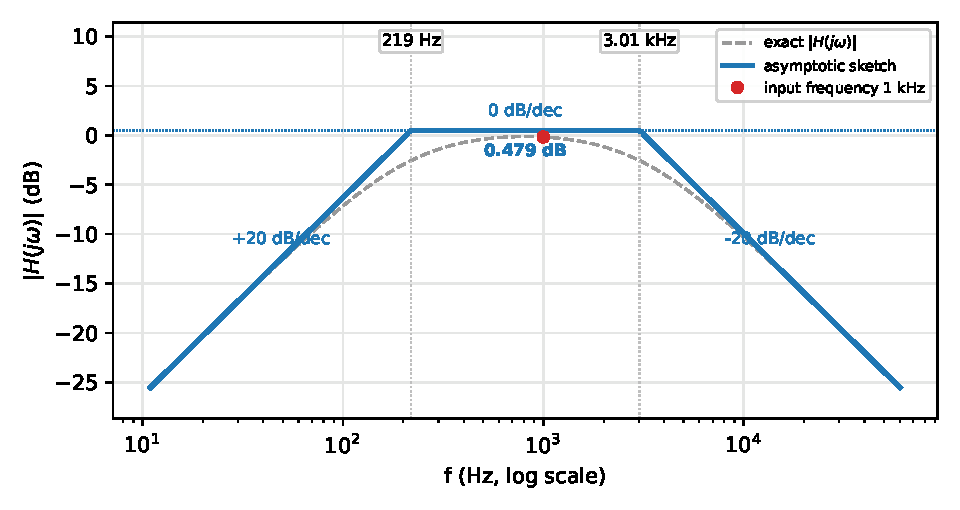
\includegraphics[width=0.78\linewidth,height=6.5cm,keepaspectratio]{p11_bode}\end{center}

{\small Blue: the straight-line sketch you are expected to draw. Dashed grey: the exact curve (about 3\,dB below the corner of an isolated pole). Red dot: the input frequency of Step 7.}
\solstep{7}{Steady-state output}The input is $V_i(t) = 2\sin\left(2\pi\cdot 1000\,t\right)$, so $\omega_{in} = 2\pi\cdot 1000 = 6280$\,rad/s. Put $s=j\omega_{in}$ in each factor (tool T5): magnitudes multiply, angles add.
{\small Rules: $\left|\frac{s}{s+p}\right| = \frac{\omega}{\sqrt{\omega^2+p^2}}$, $\angle = \frac{\pi}{2}-\tan^{-1}\frac{\omega}{p}$;\quad $\left|\frac{1}{1+s/p}\right| = \frac{1}{\sqrt{1+(\omega/p)^2}}$, $\angle = -\tan^{-1}\frac{\omega}{p}$;\quad $\left|1+\frac{s}{z}\right| = \sqrt{1+(\omega/z)^2}$, $\angle = \tan^{-1}\frac{\omega}{z}$;\quad a negative $K$ adds $-\pi$.}
\begin{center}\renewcommand{\arraystretch}{1.35}
\begin{tabular}{ccc}
\toprule
factor & magnitude & angle (rad) \\
\midrule
$1.06$ & $1.057$ & $0$ \\
$\rule[-1.1em]{0pt}{2.8em}\dfrac{s}{s+2\pi\cdot 219}$ & $0.9769$ & $0.215$ \\
$\rule[-1.7em]{0pt}{4em}\dfrac{1}{1+\dfrac{s}{2\pi\cdot 3.01\mathrm{k}}}$ & $0.9491$ & $-0.321$ \\
\textbf{total} & $\mathbf{0.9798}$ (product) & $\mathbf{-0.105}$ (sum) \\
\bottomrule
\end{tabular}\end{center}

\begin{align*}
|H(j\omega_{in})| &= 0.98, \qquad \angle H(j\omega_{in}) = -0.105\ \mathrm{rad} \\
v_{o,ac}(t) &= 0.98\times 2\,\sin\left(2\pi\cdot 1000\,t - 0.105\right) = 1.96\,\sin\left(2\pi\cdot 1000\,t - 0.105\right)
\end{align*}

Add the DC part from Step 2 (superposition):
\[
\boxed{V_o(t) = -0.923 + 1.96\,\sin\left(2\pi\cdot 1000\,t - 0.105\right)\ \mathrm{V}}
\]

\begin{ansbox}
$H(s) = 1.06\,\dfrac{s}{s+2\pi\cdot 219}\,\dfrac{1}{1+\dfrac{s}{2\pi\cdot 3.01\mathrm{k}}}$\quad (corners: 219 Hz, 3.01 kHz)\\[4pt]
$V_o(t) = -0.923 + 1.96\,\sin\left(2\pi\cdot 1000\,t - 0.105\right)\ \mathrm{V}$
\end{ansbox}

\newpage
\subsection*{Solution 1B.12 \hfill Medium}
\begin{center}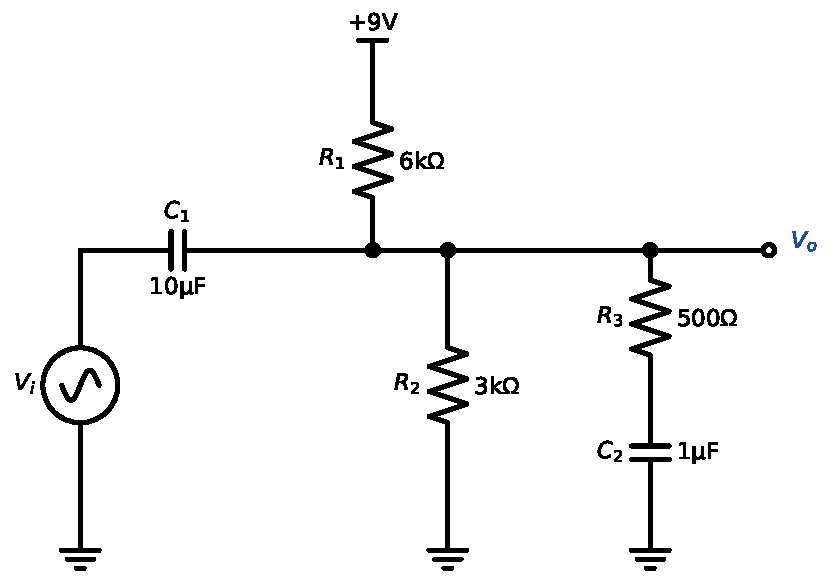
\includegraphics[width=0.8\linewidth,height=4.5cm,keepaspectratio]{p12_circuit}\end{center}
\solstep{1}{Identify the sources}Independent sources: the AC input $V_i(t)$ and the DC supplies $+9\,\mathrm{V}$. Because there are both DC and AC sources, use superposition: $V_o(t) = V_{o,dc} + v_{o,ac}(t)$. Solve the DC circuit (Step 2) and the AC circuit (Steps 3--7) separately, then add.
\solstep{2}{DC circuit $\Rightarrow V_{o,dc}$}DC rules: the AC input is set to zero ($V_i=0$: a wire to ground); every capacitor is an open circuit ($C_{1}, C_{2}$). Only the part of the circuit that is still connected to $V_o$ matters:
\begin{center}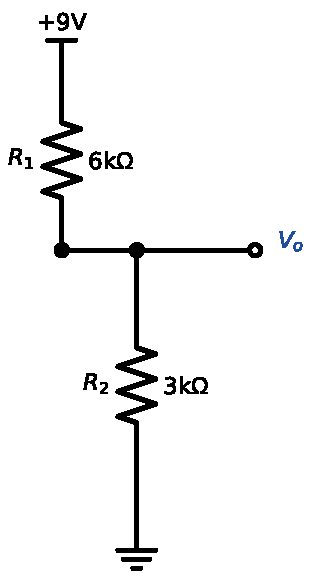
\includegraphics[width=0.55\linewidth,height=5cm,keepaspectratio]{p12_dc}\end{center}

Reduce the circuit with one tool only --- the \emph{divider between two voltages} (tool T3) --- walking toward $V_o$ and keeping a Thevenin pair $(V_{th},R_{th})$ for everything already visited.
\begin{enumerate}[leftmargin=*,itemsep=2pt]
\item Start at the input node: since $V_i=0$ it is tied to ground, i.e. it is an ideal $0\,\mathrm{V}$ source: $(V_{th},R_{th})=(0\,\mathrm{V},\,0\,\Omega)$.
\item $C_{1}$ is a capacitor $\Rightarrow$ open at DC. No DC current can cross it, so everything on its left is disconnected: start fresh after it.
\item Finally, collect everything at the output node $V_o$.
\item First DC path here: $R_{1}$ to the $+9\,\mathrm{V}$ supply, so $(V_{th},R_{th}) = (9\,\mathrm{V},\ 6\,\mathrm{k}\Omega)$.
\item Add $R_{2}$ to ground. Divider between $V_a=9\,\mathrm{V}$ (through $R_a=6\,\mathrm{k}\Omega$) and $V_b=0\,\mathrm{V}$ (through $R_b=3\,\mathrm{k}\Omega$):\[
V_{th} = V_b + (V_a-V_b)\frac{R_b}{R_a+R_b} = 0 + \left(9 - (0)\right)\frac{3\,\mathrm{k}}{6\,\mathrm{k} + 3\,\mathrm{k}} = 3\,\mathrm{V},\qquad R_{th} = R_a\parallel R_b = 2\,\mathrm{k}\Omega
\]

\item $R_{3} + C_{2}$ (at $V_{o}$) contains a capacitor: open at DC, ignore it.
\end{enumerate}

\[
\boxed{V_{o,dc} = 3\,\mathrm{V}}
\]

\solstep{3}{AC circuit}Set every DC supply to zero: each supply rail becomes AC ground. Replace every capacitor by $\frac{1}{sC}$ and every inductor by $sL$.
\begin{itemize}[leftmargin=*,itemsep=2pt]
\item $R_{1}$, $R_{2}$ both go from the same node to (AC) ground, so they are in parallel: $R_{12} = R_{1} \parallel R_{2} = 6\,\mathrm{k} \parallel 3\,\mathrm{k} = 2\,\mathrm{k}\Omega$.
\end{itemize}

AC equivalent circuit (nodes named for the next step):
\begin{center}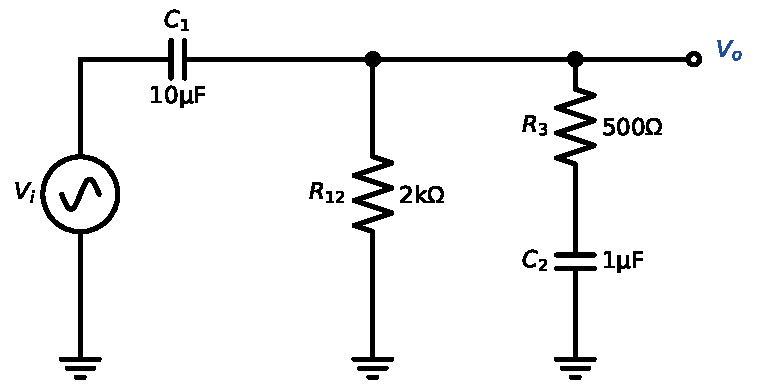
\includegraphics[width=0.95\linewidth,height=5.2cm,keepaspectratio]{p12_ac}\end{center}

\solstep{4}{Transfer function by a chain of dividers}Walk from the input to the output through the named nodes: $V_{i} \to V_{o}$. There is a single link, so $H(s)$ is just one voltage divider (tool T2).
Impedances seen \emph{looking right} from a node (everything from that node to ground, excluding what is on its left). Compute them from the far right toward the input:
\begin{align*}
Z_{o} &= R_{12} \parallel \left(R_{3} + \frac{1}{sC_{2}}\right) = \dfrac{400\,s + 8\times 10^{5}}{s + 400}
\end{align*}

Now each link. {\small (Algebra tip: to simplify a fraction that contains fractions, multiply its top and bottom by every inner denominator; then divide top and bottom by the leading coefficient of the denominator so that it starts with a plain $s^n$.)}
\begin{align*}
\frac{V_{o}}{V_{i}} &= \frac{Z_{o}}{\frac{1}{sC_{1}} + Z_{o}} = \dfrac{s^{2} + 2000\,s}{s^{2} + 2250\,s + 10^{5}}
\end{align*}

So:\[
H(s) = \dfrac{s^{2} + 2000\,s}{s^{2} + 2250\,s + 10^{5}}
\]

\solstep{5}{Standard (Bode-ready) form}Find the roots. Every root $s=-p$ of the denominator is a \emph{pole}, every root $s=-z$ of the numerator is a \emph{zero}; $|p|$ and $|z|$ are the corner frequencies (rad/s).
\begin{itemize}[leftmargin=*,itemsep=2pt]
\item Numerator: it has the factor $s$ $\Rightarrow$ 1 zero at $s=0$.
\item Numerator (after taking out the $s$ factor): $s + 2000$; $s + 2000 = 0 \Rightarrow s = -2000$.
\item Denominator: $s^{2} + 2250\,s + 10^{5}$; quadratic formula:\[
s = \frac{-2250 \pm \sqrt{(2250)^2 - 4(10^{5})}}{2} = \frac{-2250 \pm 2160}{2} \Rightarrow s = -45.4,\ -2200
\]

\end{itemize}

Factored form (leading coefficient in front):
\[
H(s) = 1\,\dfrac{s(s+2000)}{(s+45.4)(s+2200)}
\]

Bode-ready form: rewrite every $(s+p) = p\left(1+\frac{s}{p}\right)$ and $(s+z) = z\left(1+\frac{s}{z}\right)$, and collect all constants into $K$. Each $s$ in the numerator is paired with one of the \emph{lowest} poles as $\frac{s}{s+p}$ (that factor is $\approx 1$ above $p$). Then every factor except $K$ is $\approx 1$ inside the pass-band:
\[
H(s) = 0.907\,\dfrac{s}{s+2\pi\cdot 7.22}\,\left(1+\dfrac{s}{2\pi\cdot 318}\right)\,\dfrac{1}{1+\dfrac{s}{2\pi\cdot 351}},\qquad K = 0.907
\]

\begin{center}\renewcommand{\arraystretch}{1.35}
\begin{tabular}{cccc}
\toprule
type & $\omega_c$ (rad/s) & $f_c=\omega_c/2\pi$ & slope change \\
\midrule
pole & $45.4$ & 7.22 Hz & $-20$ dB/dec \\
zero & $2000$ & 318 Hz & $+20$ dB/dec \\
pole & $2200$ & 351 Hz & $-20$ dB/dec \\
\bottomrule
\end{tabular}\end{center}

\solstep{6}{Magnitude Bode plot}Below every corner $|H(s)|\approx 0.02\,s$, so the plot starts with a slope of $+20$\,dB/dec. Then, moving right, each pole bends the line down by 20\,dB/dec and each zero bends it up by 20\,dB/dec (tool T6):
\begin{center}\renewcommand{\arraystretch}{1.35}
\begin{tabular}{lcl}
\toprule
frequency range & slope & asymptote level \\
\midrule
$f<$ 7.22 Hz & $+20$ dB/dec & -0.846 dB at end \\
7.22 Hz -- 318 Hz & $0$ dB/dec (flat) & -0.846 dB at start, -0.846 dB at end \\
318 Hz -- 351 Hz & $+20$ dB/dec & -0.846 dB at start, 0 dB at end \\
$f>$ 351 Hz & $0$ dB/dec (flat) & 0 dB at start \\
\bottomrule
\end{tabular}\end{center}

\begin{center}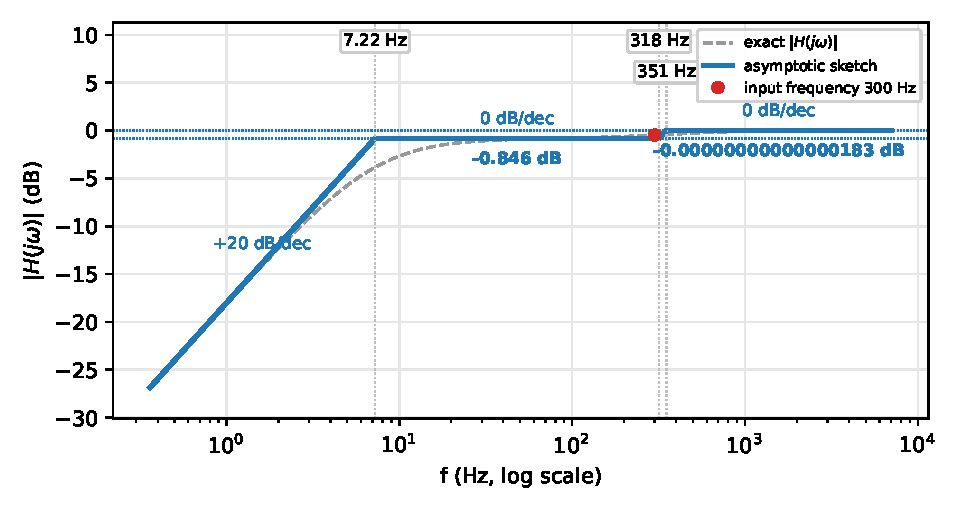
\includegraphics[width=0.78\linewidth,height=6.5cm,keepaspectratio]{p12_bode}\end{center}

{\small Blue: the straight-line sketch you are expected to draw. Dashed grey: the exact curve (about 3\,dB below the corner of an isolated pole). Red dot: the input frequency of Step 7.}
\solstep{7}{Steady-state output}The input is $V_i(t) = 0.4\sin\left(2\pi\cdot 300\,t\right)$, so $\omega_{in} = 2\pi\cdot 300 = 1880$\,rad/s. Put $s=j\omega_{in}$ in each factor (tool T5): magnitudes multiply, angles add.
{\small Rules: $\left|\frac{s}{s+p}\right| = \frac{\omega}{\sqrt{\omega^2+p^2}}$, $\angle = \frac{\pi}{2}-\tan^{-1}\frac{\omega}{p}$;\quad $\left|\frac{1}{1+s/p}\right| = \frac{1}{\sqrt{1+(\omega/p)^2}}$, $\angle = -\tan^{-1}\frac{\omega}{p}$;\quad $\left|1+\frac{s}{z}\right| = \sqrt{1+(\omega/z)^2}$, $\angle = \tan^{-1}\frac{\omega}{z}$;\quad a negative $K$ adds $-\pi$.}
\begin{center}\renewcommand{\arraystretch}{1.35}
\begin{tabular}{ccc}
\toprule
factor & magnitude & angle (rad) \\
\midrule
$0.907$ & $0.9072$ & $0$ \\
$\rule[-1.1em]{0pt}{2.8em}\dfrac{s}{s+2\pi\cdot 7.22}$ & $0.9997$ & $0.0241$ \\
$\rule[-1.1em]{0pt}{2.8em}\left(1+\dfrac{s}{2\pi\cdot 318}\right)$ & $1.374$ & $0.756$ \\
$\rule[-1.7em]{0pt}{4em}\dfrac{1}{1+\dfrac{s}{2\pi\cdot 351}}$ & $0.7601$ & $-0.707$ \\
\textbf{total} & $\mathbf{0.9472}$ (product) & $\mathbf{0.0725}$ (sum) \\
\bottomrule
\end{tabular}\end{center}

\begin{align*}
|H(j\omega_{in})| &= 0.947, \qquad \angle H(j\omega_{in}) = 0.0725\ \mathrm{rad} \\
v_{o,ac}(t) &= 0.947\times 0.4\,\sin\left(2\pi\cdot 300\,t + 0.0725\right) = 0.379\,\sin\left(2\pi\cdot 300\,t + 0.0725\right)
\end{align*}

Add the DC part from Step 2 (superposition):
\[
\boxed{V_o(t) = 3 + 0.379\,\sin\left(2\pi\cdot 300\,t + 0.0725\right)\ \mathrm{V}}
\]

\begin{ansbox}
$H(s) = 0.907\,\dfrac{s}{s+2\pi\cdot 7.22}\,\left(1+\dfrac{s}{2\pi\cdot 318}\right)\,\dfrac{1}{1+\dfrac{s}{2\pi\cdot 351}}$\quad (corners: 7.22 Hz, 318 Hz, 351 Hz)\\[4pt]
$V_o(t) = 3 + 0.379\,\sin\left(2\pi\cdot 300\,t + 0.0725\right)\ \mathrm{V}$
\end{ansbox}

\newpage
\subsection*{Solution 1B.13 \hfill Hard}
\begin{center}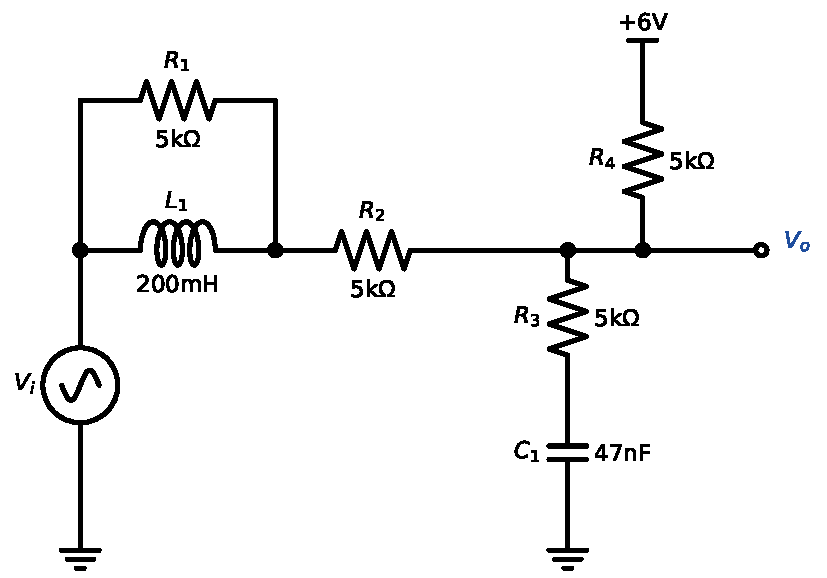
\includegraphics[width=0.8\linewidth,height=4.5cm,keepaspectratio]{p13_circuit}\end{center}
\solstep{1}{Identify the sources}Independent sources: the AC input $V_i(t)$ and the DC supplies $+6\,\mathrm{V}$. Because there are both DC and AC sources, use superposition: $V_o(t) = V_{o,dc} + v_{o,ac}(t)$. Solve the DC circuit (Step 2) and the AC circuit (Steps 3--7) separately, then add.
\solstep{2}{DC circuit $\Rightarrow V_{o,dc}$}DC rules: the AC input is set to zero ($V_i=0$: a wire to ground); every capacitor is an open circuit ($C_{1}$); every inductor is a short circuit ($L_{1}$). Only the part of the circuit that is still connected to $V_o$ matters:
\begin{center}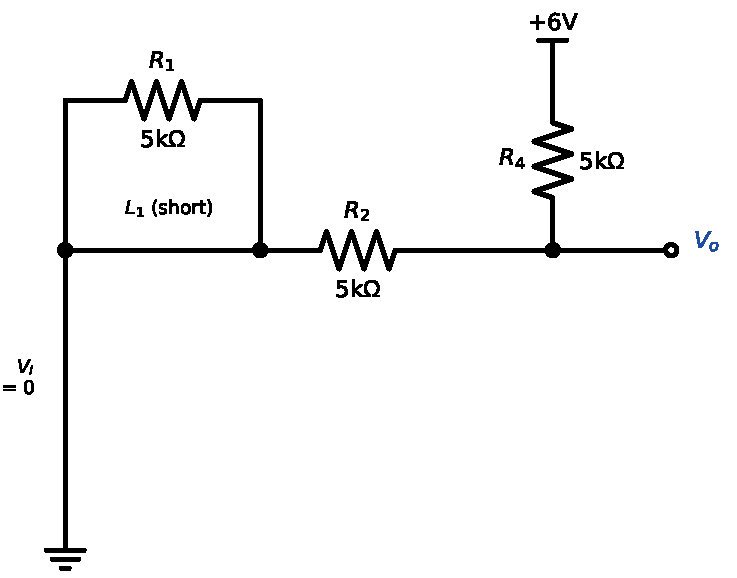
\includegraphics[width=0.55\linewidth,height=5cm,keepaspectratio]{p13_dc}\end{center}

Reduce the circuit with one tool only --- the \emph{divider between two voltages} (tool T3) --- walking toward $V_o$ and keeping a Thevenin pair $(V_{th},R_{th})$ for everything already visited.
\begin{enumerate}[leftmargin=*,itemsep=2pt]
\item Start at the input node: since $V_i=0$ it is tied to ground, i.e. it is an ideal $0\,\mathrm{V}$ source: $(V_{th},R_{th})=(0\,\mathrm{V},\,0\,\Omega)$.
\item $L_{1} \parallel R_{1}$ is a short at DC (inductor), so the pair is unchanged.
\item Walk through $R_{2}$ ($5\,\mathrm{k}\Omega$ at DC). A series resistor just adds to $R_{th}$: $(V_{th},R_{th}) = (0\,\mathrm{V},\ 5\,\mathrm{k}\Omega)$.
\item Finally, collect everything at the output node $V_o$.
\item $R_{3} + C_{1}$ (at $V_{o}$) contains a capacitor: open at DC, ignore it.
\item Add $R_{4}$ to the $+6\,\mathrm{V}$ supply. Divider between $V_a=0\,\mathrm{V}$ (through $R_a=5\,\mathrm{k}\Omega$) and $V_b=6\,\mathrm{V}$ (through $R_b=5\,\mathrm{k}\Omega$):\[
V_{th} = V_b + (V_a-V_b)\frac{R_b}{R_a+R_b} = 6 + \left(0 - (6)\right)\frac{5\,\mathrm{k}}{5\,\mathrm{k} + 5\,\mathrm{k}} = 3\,\mathrm{V},\qquad R_{th} = R_a\parallel R_b = 2.5\,\mathrm{k}\Omega
\]

\end{enumerate}

\[
\boxed{V_{o,dc} = 3\,\mathrm{V}}
\]

\solstep{3}{AC circuit}Set every DC supply to zero: each supply rail becomes AC ground. Replace every capacitor by $\frac{1}{sC}$ and every inductor by $sL$.
AC equivalent circuit (nodes named for the next step):
\begin{center}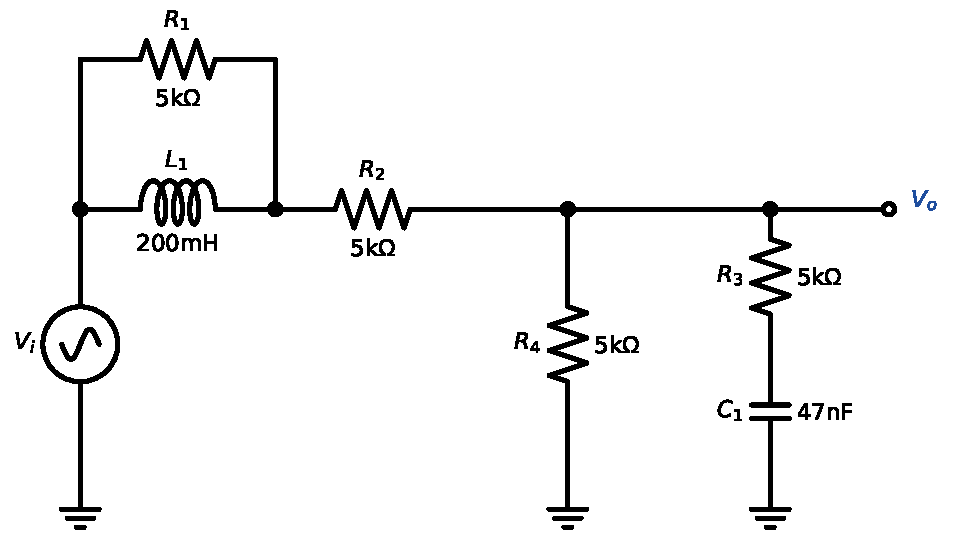
\includegraphics[width=0.95\linewidth,height=5.2cm,keepaspectratio]{p13_ac}\end{center}

\solstep{4}{Transfer function by a chain of dividers}Walk from the input to the output through the named nodes: $V_{i} \to V_{o}$. There is a single link, so $H(s)$ is just one voltage divider (tool T2).
Impedances seen \emph{looking right} from a node (everything from that node to ground, excluding what is on its left). Compute them from the far right toward the input:
\begin{align*}
Z_{o} &= R_{4} \parallel \left(R_{3} + \frac{1}{sC_{1}}\right) = \dfrac{2500\,s + 1.06\times 10^{7}}{s + 2130}
\end{align*}

Now each link. {\small (Algebra tip: to simplify a fraction that contains fractions, multiply its top and bottom by every inner denominator; then divide top and bottom by the leading coefficient of the denominator so that it starts with a plain $s^n$.)}
\begin{align*}
\frac{V_{o}}{V_{i}} &= \frac{Z_{o}}{\left(sL_{1} \parallel R_{1}\right) + R_{2} + Z_{o}} = \dfrac{0.2\,s^{2} + 5850\,s + 2.13\times 10^{7}}{s^{2} + 17600\,s + 4.26\times 10^{7}}
\end{align*}

So:\[
H(s) = \dfrac{0.2\,s^{2} + 5850\,s + 2.13\times 10^{7}}{s^{2} + 17600\,s + 4.26\times 10^{7}}
\]

\solstep{5}{Standard (Bode-ready) form}Find the roots. Every root $s=-p$ of the denominator is a \emph{pole}, every root $s=-z$ of the numerator is a \emph{zero}; $|p|$ and $|z|$ are the corner frequencies (rad/s).
\begin{itemize}[leftmargin=*,itemsep=2pt]
\item Numerator: $0.2\,s^{2} + 5850\,s + 2.13\times 10^{7}$; divide by the leading coefficient $0.2$ (this does not move the roots): $s^{2} + 29300\,s + 1.06\times 10^{8}$; quadratic formula:\[
s = \frac{-29300 \pm \sqrt{(29300)^2 - 4(1.06\times 10^{8})}}{2} = \frac{-29300 \pm 20700}{2} \Rightarrow s = -4260,\ -25000
\]

\item Denominator: $s^{2} + 17600\,s + 4.26\times 10^{7}$; quadratic formula:\[
s = \frac{-17600 \pm \sqrt{(17600)^2 - 4(4.26\times 10^{7})}}{2} = \frac{-17600 \pm 11700}{2} \Rightarrow s = -2910,\ -14600
\]

\end{itemize}

Factored form (leading coefficient in front):
\[
H(s) = 0.2\,\dfrac{(s+4260)(s+25000)}{(s+2910)(s+14600)}
\]

Bode-ready form: rewrite every $(s+p) = p\left(1+\frac{s}{p}\right)$ and $(s+z) = z\left(1+\frac{s}{z}\right)$, and collect all constants into $K$. Then every factor except $K$ is $\approx 1$ inside the pass-band:
\[
H(s) = 0.5\,\dfrac{1}{1+\dfrac{s}{2\pi\cdot 462}}\,\left(1+\dfrac{s}{2\pi\cdot 677}\right)\,\dfrac{1}{1+\dfrac{s}{2\pi\cdot 2.33\mathrm{k}}}\,\left(1+\dfrac{s}{2\pi\cdot 3.98\mathrm{k}}\right),\qquad K = 0.5
\]

\begin{center}\renewcommand{\arraystretch}{1.35}
\begin{tabular}{cccc}
\toprule
type & $\omega_c$ (rad/s) & $f_c=\omega_c/2\pi$ & slope change \\
\midrule
pole & $2910$ & 462 Hz & $-20$ dB/dec \\
zero & $4260$ & 677 Hz & $+20$ dB/dec \\
pole & $14600$ & 2.33 kHz & $-20$ dB/dec \\
zero & $25000$ & 3.98 kHz & $+20$ dB/dec \\
\bottomrule
\end{tabular}\end{center}

\solstep{6}{Magnitude Bode plot}Below every corner, all factors are $\approx$ constant: $|H| \approx 0.5$ $= -6.02$\,dB (flat, 0 dB/dec). Then, moving right, each pole bends the line down by 20\,dB/dec and each zero bends it up by 20\,dB/dec (tool T6):
\begin{center}\renewcommand{\arraystretch}{1.35}
\begin{tabular}{lcl}
\toprule
frequency range & slope & asymptote level \\
\midrule
$f<$ 462 Hz & $0$ dB/dec (flat) & -6.02 dB at end \\
462 Hz -- 677 Hz & $-20$ dB/dec & -6.02 dB at start, -9.34 dB at end \\
677 Hz -- 2.33 kHz & $0$ dB/dec (flat) & -9.34 dB at start, -9.34 dB at end \\
2.33 kHz -- 3.98 kHz & $-20$ dB/dec & -9.34 dB at start, -14 dB at end \\
$f>$ 3.98 kHz & $0$ dB/dec (flat) & -14 dB at start \\
\bottomrule
\end{tabular}\end{center}

\begin{center}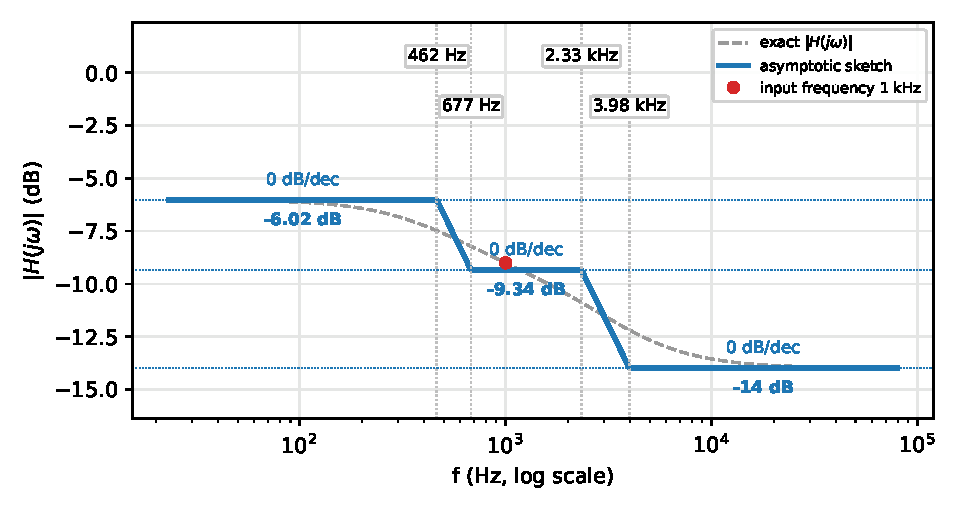
\includegraphics[width=0.78\linewidth,height=6.5cm,keepaspectratio]{p13_bode}\end{center}

{\small Blue: the straight-line sketch you are expected to draw. Dashed grey: the exact curve (about 3\,dB below the corner of an isolated pole). Red dot: the input frequency of Step 7.}
\solstep{7}{Steady-state output}The input is $V_i(t) = 1.5\sin\left(2\pi\cdot 1000\,t+\frac{\pi}{4}\right)$, so $\omega_{in} = 2\pi\cdot 1000 = 6280$\,rad/s. Put $s=j\omega_{in}$ in each factor (tool T5): magnitudes multiply, angles add.
{\small Rules: $\left|\frac{s}{s+p}\right| = \frac{\omega}{\sqrt{\omega^2+p^2}}$, $\angle = \frac{\pi}{2}-\tan^{-1}\frac{\omega}{p}$;\quad $\left|\frac{1}{1+s/p}\right| = \frac{1}{\sqrt{1+(\omega/p)^2}}$, $\angle = -\tan^{-1}\frac{\omega}{p}$;\quad $\left|1+\frac{s}{z}\right| = \sqrt{1+(\omega/z)^2}$, $\angle = \tan^{-1}\frac{\omega}{z}$;\quad a negative $K$ adds $-\pi$.}
\begin{center}\renewcommand{\arraystretch}{1.35}
\begin{tabular}{ccc}
\toprule
factor & magnitude & angle (rad) \\
\midrule
$0.5$ & $0.5$ & $0$ \\
$\rule[-1.7em]{0pt}{4em}\dfrac{1}{1+\dfrac{s}{2\pi\cdot 462}}$ & $0.4197$ & $-1.14$ \\
$\rule[-1.1em]{0pt}{2.8em}\left(1+\dfrac{s}{2\pi\cdot 677}\right)$ & $1.783$ & $0.975$ \\
$\rule[-1.7em]{0pt}{4em}\dfrac{1}{1+\dfrac{s}{2\pi\cdot 2.33\mathrm{k}}}$ & $0.919$ & $-0.405$ \\
$\rule[-1.1em]{0pt}{2.8em}\left(1+\dfrac{s}{2\pi\cdot 3.98\mathrm{k}}\right)$ & $1.031$ & $0.246$ \\
\textbf{total} & $\mathbf{0.3546}$ (product) & $\mathbf{-0.321}$ (sum) \\
\bottomrule
\end{tabular}\end{center}

\begin{align*}
|H(j\omega_{in})| &= 0.355, \qquad \angle H(j\omega_{in}) = -0.321\ \mathrm{rad} \\
v_{o,ac}(t) &= 0.355\times 1.5\,\sin\left(2\pi\cdot 1000\,t + 0.464\right) = 0.532\,\sin\left(2\pi\cdot 1000\,t + 0.464\right)
\end{align*}

(phase: $\theta + \angle H = \frac{\pi}{4} + (-0.321) = 0.464$\,rad.)
Add the DC part from Step 2 (superposition):
\[
\boxed{V_o(t) = 3 + 0.532\,\sin\left(2\pi\cdot 1000\,t + 0.464\right)\ \mathrm{V}}
\]

\begin{ansbox}
$H(s) = 0.5\,\dfrac{1}{1+\dfrac{s}{2\pi\cdot 462}}\,\left(1+\dfrac{s}{2\pi\cdot 677}\right)\,\dfrac{1}{1+\dfrac{s}{2\pi\cdot 2.33\mathrm{k}}}\,\left(1+\dfrac{s}{2\pi\cdot 3.98\mathrm{k}}\right)$\quad (corners: 462 Hz, 677 Hz, 2.33 kHz, 3.98 kHz)\\[4pt]
$V_o(t) = 3 + 0.532\,\sin\left(2\pi\cdot 1000\,t + 0.464\right)\ \mathrm{V}$
\end{ansbox}

\newpage
\subsection*{Solution 1B.14 \hfill Hard}
\begin{center}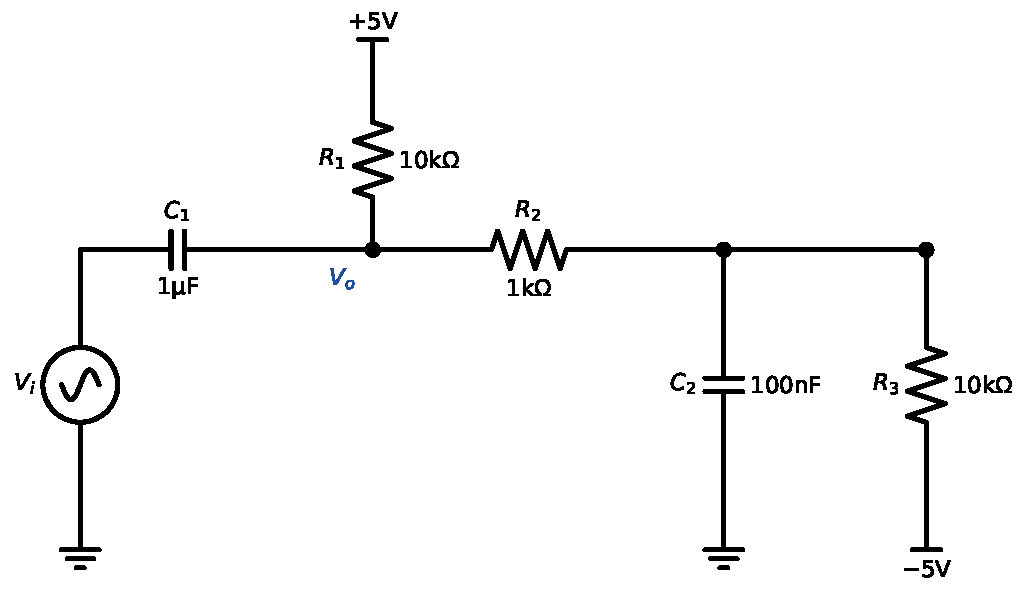
\includegraphics[width=0.8\linewidth,height=4.5cm,keepaspectratio]{p14_circuit}\end{center}
\solstep{1}{Identify the sources}Independent sources: the AC input $V_i(t)$ and the DC supplies $-5\,\mathrm{V}$, $+5\,\mathrm{V}$. Because there are both DC and AC sources, use superposition: $V_o(t) = V_{o,dc} + v_{o,ac}(t)$. Solve the DC circuit (Step 2) and the AC circuit (Steps 3--7) separately, then add.
\solstep{2}{DC circuit $\Rightarrow V_{o,dc}$}DC rules: the AC input is set to zero ($V_i=0$: a wire to ground); every capacitor is an open circuit ($C_{1}, C_{2}$). Only the part of the circuit that is still connected to $V_o$ matters:
\begin{center}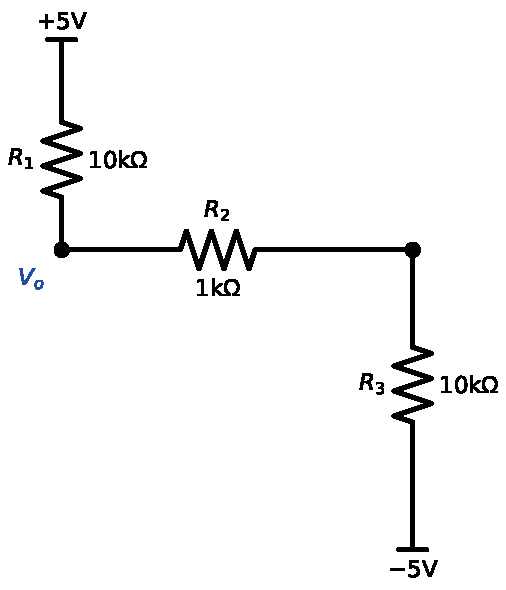
\includegraphics[width=0.55\linewidth,height=5cm,keepaspectratio]{p14_dc}\end{center}

Reduce the circuit with one tool only --- the \emph{divider between two voltages} (tool T3) --- walking toward $V_o$ and keeping a Thevenin pair $(V_{th},R_{th})$ for everything already visited.
\begin{enumerate}[leftmargin=*,itemsep=2pt]
\item Start at the input node: since $V_i=0$ it is tied to ground, i.e. it is an ideal $0\,\mathrm{V}$ source: $(V_{th},R_{th})=(0\,\mathrm{V},\,0\,\Omega)$.
\item $C_{1}$ is a capacitor $\Rightarrow$ open at DC. No DC current can cross it, so everything on its left is disconnected: start fresh after it.
\item Now reduce the part to the \emph{right} of $V_o$ the same way, starting at the far right end and moving toward $V_o$.
\item $C_{2}$ (at $V_{1}$) is a capacitor: open at DC, ignore it.
\item First DC path here: $R_{3}$ to the $-5\,\mathrm{V}$ supply, so $(V_{th},R_{th}) = (-5\,\mathrm{V},\ 10\,\mathrm{k}\Omega)$.
\item Walk through $R_{2}$ ($1\,\mathrm{k}\Omega$ at DC). A series resistor just adds to $R_{th}$: $(V_{th},R_{th}) = (-5\,\mathrm{V},\ 11\,\mathrm{k}\Omega)$.
\item Finally, collect everything at the output node $V_o$.
\item First DC path here: $R_{1}$ to the $+5\,\mathrm{V}$ supply, so $(V_{th},R_{th}) = (5\,\mathrm{V},\ 10\,\mathrm{k}\Omega)$.
\item $V_o$ sits between the left pair $(5\,\mathrm{V},\ 10\,\mathrm{k}\Omega)$ and the right pair $(-5\,\mathrm{V},\ 11\,\mathrm{k}\Omega)$:\[
V_{o,dc} = -5 + \left(5 - (-5)\right)\frac{11\,\mathrm{k}}{10\,\mathrm{k} + 11\,\mathrm{k}} = 238\,\mathrm{m}\mathrm{V}
\]

\end{enumerate}

\[
\boxed{V_{o,dc} = 238\,\mathrm{m}\mathrm{V}}
\]

\solstep{3}{AC circuit}Set every DC supply to zero: each supply rail becomes AC ground. Replace every capacitor by $\frac{1}{sC}$ and every inductor by $sL$.
AC equivalent circuit (nodes named for the next step):
\begin{center}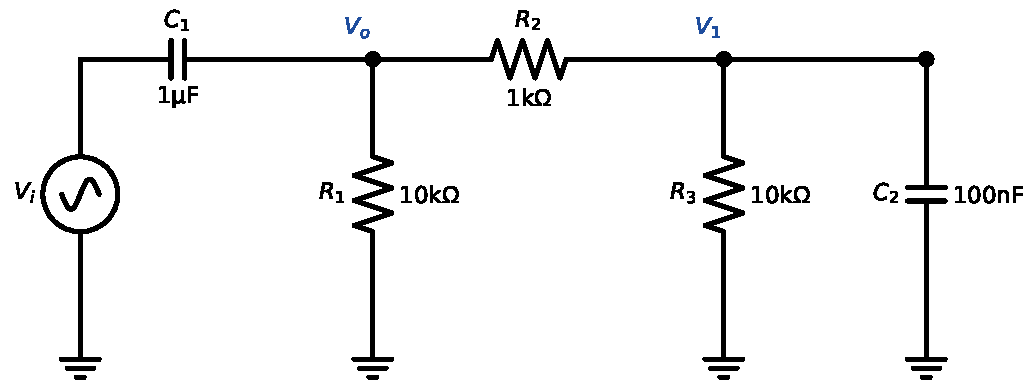
\includegraphics[width=0.95\linewidth,height=5.2cm,keepaspectratio]{p14_ac}\end{center}

\solstep{4}{Transfer function by a chain of dividers}Walk from the input to the output through the named nodes: $V_{i} \to V_{o}$. There is a single link, so $H(s)$ is just one voltage divider (tool T2).
Impedances seen \emph{looking right} from a node (everything from that node to ground, excluding what is on its left). Compute them from the far right toward the input:
\begin{align*}
Z_{1} &= R_{3} \parallel \frac{1}{sC_{2}} = \dfrac{10^{7}}{s + 1000} \\
Z_{o} &= R_{1} \parallel \left(R_{2} + Z_{1}\right) = \dfrac{909\,s + 10^{7}}{s + 1910}
\end{align*}

Now each link. {\small (Algebra tip: to simplify a fraction that contains fractions, multiply its top and bottom by every inner denominator; then divide top and bottom by the leading coefficient of the denominator so that it starts with a plain $s^n$.)}
\begin{align*}
\frac{V_{o}}{V_{i}} &= \frac{Z_{o}}{\frac{1}{sC_{1}} + Z_{o}} = \dfrac{s^{2} + 11000\,s}{s^{2} + 12100\,s + 2.1\times 10^{6}}
\end{align*}

So:\[
H(s) = \dfrac{s^{2} + 11000\,s}{s^{2} + 12100\,s + 2.1\times 10^{6}}
\]

\solstep{5}{Standard (Bode-ready) form}Find the roots. Every root $s=-p$ of the denominator is a \emph{pole}, every root $s=-z$ of the numerator is a \emph{zero}; $|p|$ and $|z|$ are the corner frequencies (rad/s).
\begin{itemize}[leftmargin=*,itemsep=2pt]
\item Numerator: it has the factor $s$ $\Rightarrow$ 1 zero at $s=0$.
\item Numerator (after taking out the $s$ factor): $s + 11000$; $s + 11000 = 0 \Rightarrow s = -11000$.
\item Denominator: $s^{2} + 12100\,s + 2.1\times 10^{6}$; quadratic formula:\[
s = \frac{-12100 \pm \sqrt{(12100)^2 - 4(2.1\times 10^{6})}}{2} = \frac{-12100 \pm 11700}{2} \Rightarrow s = -176,\ -11900
\]

\end{itemize}

Factored form (leading coefficient in front):
\[
H(s) = 1\,\dfrac{s(s+11000)}{(s+176)(s+11900)}
\]

Bode-ready form: rewrite every $(s+p) = p\left(1+\frac{s}{p}\right)$ and $(s+z) = z\left(1+\frac{s}{z}\right)$, and collect all constants into $K$. Each $s$ in the numerator is paired with one of the \emph{lowest} poles as $\frac{s}{s+p}$ (that factor is $\approx 1$ above $p$). Then every factor except $K$ is $\approx 1$ inside the pass-band:
\[
H(s) = 0.923\,\dfrac{s}{s+2\pi\cdot 28}\,\left(1+\dfrac{s}{2\pi\cdot 1.75\mathrm{k}}\right)\,\dfrac{1}{1+\dfrac{s}{2\pi\cdot 1.9\mathrm{k}}},\qquad K = 0.923
\]

\begin{center}\renewcommand{\arraystretch}{1.35}
\begin{tabular}{cccc}
\toprule
type & $\omega_c$ (rad/s) & $f_c=\omega_c/2\pi$ & slope change \\
\midrule
pole & $176$ & 28 Hz & $-20$ dB/dec \\
zero & $11000$ & 1.75 kHz & $+20$ dB/dec \\
pole & $11900$ & 1.9 kHz & $-20$ dB/dec \\
\bottomrule
\end{tabular}\end{center}

\solstep{6}{Magnitude Bode plot}Below every corner $|H(s)|\approx 0.00524\,s$, so the plot starts with a slope of $+20$\,dB/dec. Then, moving right, each pole bends the line down by 20\,dB/dec and each zero bends it up by 20\,dB/dec (tool T6):
\begin{center}\renewcommand{\arraystretch}{1.35}
\begin{tabular}{lcl}
\toprule
frequency range & slope & asymptote level \\
\midrule
$f<$ 28 Hz & $+20$ dB/dec & -0.701 dB at end \\
28 Hz -- 1.75 kHz & $0$ dB/dec (flat) & -0.701 dB at start, -0.701 dB at end \\
1.75 kHz -- 1.9 kHz & $+20$ dB/dec & -0.701 dB at start, 0 dB at end \\
$f>$ 1.9 kHz & $0$ dB/dec (flat) & 0 dB at start \\
\bottomrule
\end{tabular}\end{center}

\begin{center}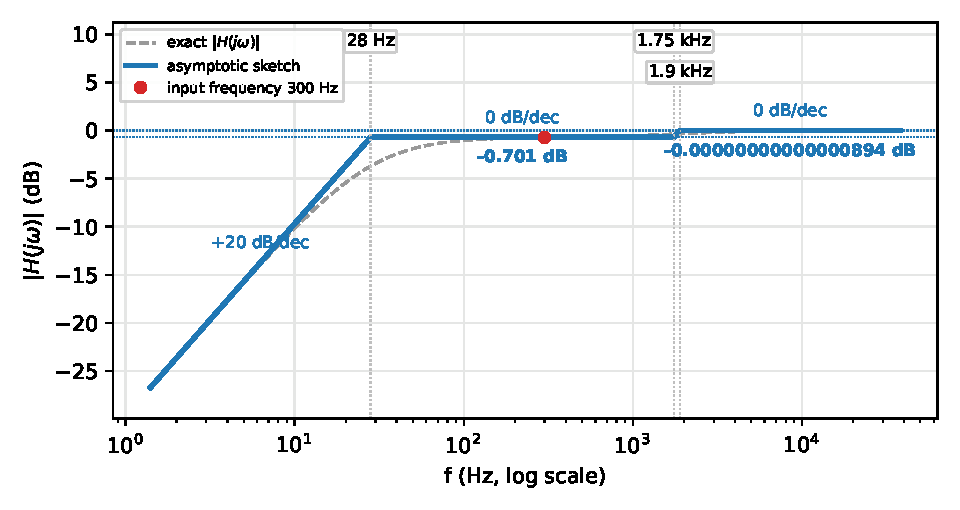
\includegraphics[width=0.78\linewidth,height=6.5cm,keepaspectratio]{p14_bode}\end{center}

{\small Blue: the straight-line sketch you are expected to draw. Dashed grey: the exact curve (about 3\,dB below the corner of an isolated pole). Red dot: the input frequency of Step 7.}
\solstep{7}{Steady-state output}The input is $V_i(t) = 0.5\sin\left(2\pi\cdot 300\,t\right)$, so $\omega_{in} = 2\pi\cdot 300 = 1880$\,rad/s. Put $s=j\omega_{in}$ in each factor (tool T5): magnitudes multiply, angles add.
{\small Rules: $\left|\frac{s}{s+p}\right| = \frac{\omega}{\sqrt{\omega^2+p^2}}$, $\angle = \frac{\pi}{2}-\tan^{-1}\frac{\omega}{p}$;\quad $\left|\frac{1}{1+s/p}\right| = \frac{1}{\sqrt{1+(\omega/p)^2}}$, $\angle = -\tan^{-1}\frac{\omega}{p}$;\quad $\left|1+\frac{s}{z}\right| = \sqrt{1+(\omega/z)^2}$, $\angle = \tan^{-1}\frac{\omega}{z}$;\quad a negative $K$ adds $-\pi$.}
\begin{center}\renewcommand{\arraystretch}{1.35}
\begin{tabular}{ccc}
\toprule
factor & magnitude & angle (rad) \\
\midrule
$0.923$ & $0.9225$ & $0$ \\
$\rule[-1.1em]{0pt}{2.8em}\dfrac{s}{s+2\pi\cdot 28}$ & $0.9957$ & $0.0932$ \\
$\rule[-1.1em]{0pt}{2.8em}\left(1+\dfrac{s}{2\pi\cdot 1.75\mathrm{k}}\right)$ & $1.015$ & $0.17$ \\
$\rule[-1.7em]{0pt}{4em}\dfrac{1}{1+\dfrac{s}{2\pi\cdot 1.9\mathrm{k}}}$ & $0.9877$ & $-0.157$ \\
\textbf{total} & $\mathbf{0.9205}$ (product) & $\mathbf{0.106}$ (sum) \\
\bottomrule
\end{tabular}\end{center}

\begin{align*}
|H(j\omega_{in})| &= 0.92, \qquad \angle H(j\omega_{in}) = 0.106\ \mathrm{rad} \\
v_{o,ac}(t) &= 0.92\times 0.5\,\sin\left(2\pi\cdot 300\,t + 0.106\right) = 0.46\,\sin\left(2\pi\cdot 300\,t + 0.106\right)
\end{align*}

Add the DC part from Step 2 (superposition):
\[
\boxed{V_o(t) = 0.238 + 0.46\,\sin\left(2\pi\cdot 300\,t + 0.106\right)\ \mathrm{V}}
\]

\begin{ansbox}
$H(s) = 0.923\,\dfrac{s}{s+2\pi\cdot 28}\,\left(1+\dfrac{s}{2\pi\cdot 1.75\mathrm{k}}\right)\,\dfrac{1}{1+\dfrac{s}{2\pi\cdot 1.9\mathrm{k}}}$\quad (corners: 28 Hz, 1.75 kHz, 1.9 kHz)\\[4pt]
$V_o(t) = 0.238 + 0.46\,\sin\left(2\pi\cdot 300\,t + 0.106\right)\ \mathrm{V}$
\end{ansbox}

\newpage
\subsection*{Solution 1B.15 \hfill Hard}
\begin{center}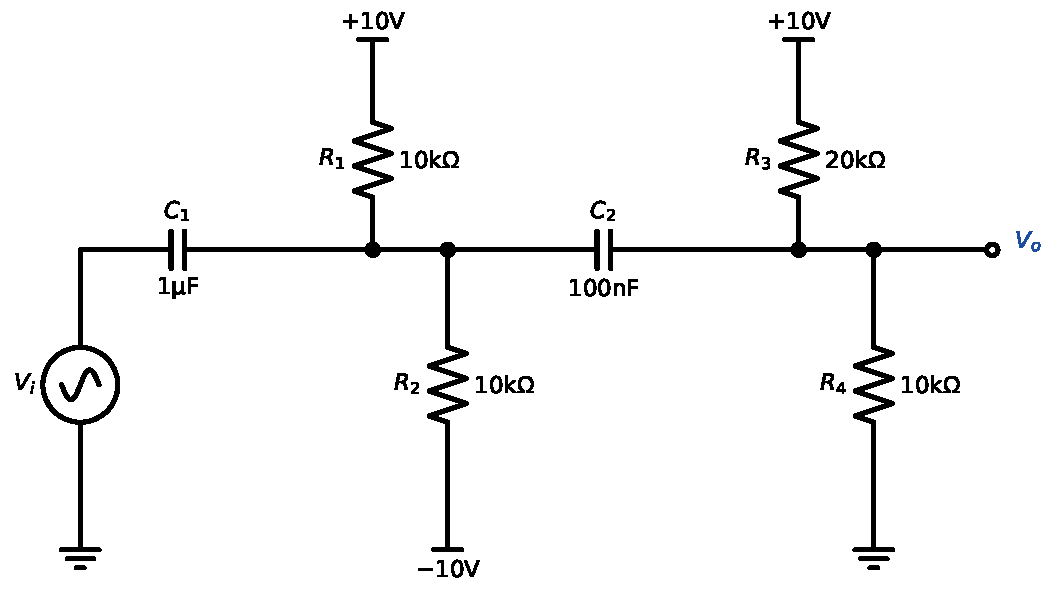
\includegraphics[width=0.8\linewidth,height=4.5cm,keepaspectratio]{p15_circuit}\end{center}
\solstep{1}{Identify the sources}Independent sources: the AC input $V_i(t)$ and the DC supplies $-10\,\mathrm{V}$, $+10\,\mathrm{V}$. Because there are both DC and AC sources, use superposition: $V_o(t) = V_{o,dc} + v_{o,ac}(t)$. Solve the DC circuit (Step 2) and the AC circuit (Steps 3--7) separately, then add.
\solstep{2}{DC circuit $\Rightarrow V_{o,dc}$}DC rules: the AC input is set to zero ($V_i=0$: a wire to ground); every capacitor is an open circuit ($C_{1}, C_{2}$). Only the part of the circuit that is still connected to $V_o$ matters:
\begin{center}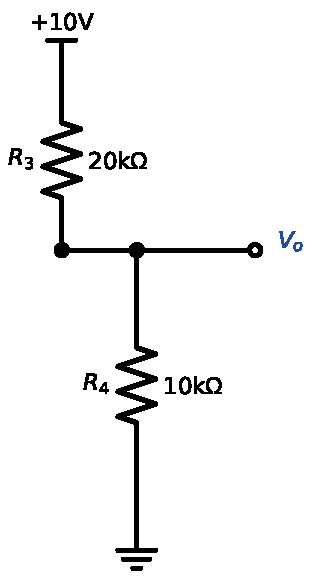
\includegraphics[width=0.55\linewidth,height=5cm,keepaspectratio]{p15_dc}\end{center}

Reduce the circuit with one tool only --- the \emph{divider between two voltages} (tool T3) --- walking toward $V_o$ and keeping a Thevenin pair $(V_{th},R_{th})$ for everything already visited.
\begin{enumerate}[leftmargin=*,itemsep=2pt]
\item Start at the input node: since $V_i=0$ it is tied to ground, i.e. it is an ideal $0\,\mathrm{V}$ source: $(V_{th},R_{th})=(0\,\mathrm{V},\,0\,\Omega)$.
\item $C_{1}$ is a capacitor $\Rightarrow$ open at DC. No DC current can cross it, so everything on its left is disconnected: start fresh after it.
\item First DC path here: $R_{1}$ to the $+10\,\mathrm{V}$ supply, so $(V_{th},R_{th}) = (10\,\mathrm{V},\ 10\,\mathrm{k}\Omega)$.
\item Add $R_{2}$ to the $-10\,\mathrm{V}$ supply. Divider between $V_a=10\,\mathrm{V}$ (through $R_a=10\,\mathrm{k}\Omega$) and $V_b=-10\,\mathrm{V}$ (through $R_b=10\,\mathrm{k}\Omega$):\[
V_{th} = V_b + (V_a-V_b)\frac{R_b}{R_a+R_b} = -10 + \left(10 - (-10)\right)\frac{10\,\mathrm{k}}{10\,\mathrm{k} + 10\,\mathrm{k}} = 0\,\mathrm{V},\qquad R_{th} = R_a\parallel R_b = 5\,\mathrm{k}\Omega
\]

\item $C_{2}$ is a capacitor $\Rightarrow$ open at DC. No DC current can cross it, so everything on its left is disconnected: start fresh after it.
\item Finally, collect everything at the output node $V_o$.
\item First DC path here: $R_{3}$ to the $+10\,\mathrm{V}$ supply, so $(V_{th},R_{th}) = (10\,\mathrm{V},\ 20\,\mathrm{k}\Omega)$.
\item Add $R_{4}$ to ground. Divider between $V_a=10\,\mathrm{V}$ (through $R_a=20\,\mathrm{k}\Omega$) and $V_b=0\,\mathrm{V}$ (through $R_b=10\,\mathrm{k}\Omega$):\[
V_{th} = V_b + (V_a-V_b)\frac{R_b}{R_a+R_b} = 0 + \left(10 - (0)\right)\frac{10\,\mathrm{k}}{20\,\mathrm{k} + 10\,\mathrm{k}} = 3.33\,\mathrm{V},\qquad R_{th} = R_a\parallel R_b = 6.67\,\mathrm{k}\Omega
\]

\end{enumerate}

\[
\boxed{V_{o,dc} = 3.33\,\mathrm{V}}
\]

\solstep{3}{AC circuit}Set every DC supply to zero: each supply rail becomes AC ground. Replace every capacitor by $\frac{1}{sC}$ and every inductor by $sL$.
\begin{itemize}[leftmargin=*,itemsep=2pt]
\item $R_{1}$, $R_{2}$ both go from the same node to (AC) ground, so they are in parallel: $R_{12} = R_{1} \parallel R_{2} = 10\,\mathrm{k} \parallel 10\,\mathrm{k} = 5\,\mathrm{k}\Omega$.
\item $R_{3}$, $R_{4}$ both go from the same node to (AC) ground, so they are in parallel: $R_{34} = R_{3} \parallel R_{4} = 20\,\mathrm{k} \parallel 10\,\mathrm{k} = 6.67\,\mathrm{k}\Omega$.
\end{itemize}

AC equivalent circuit (nodes named for the next step):
\begin{center}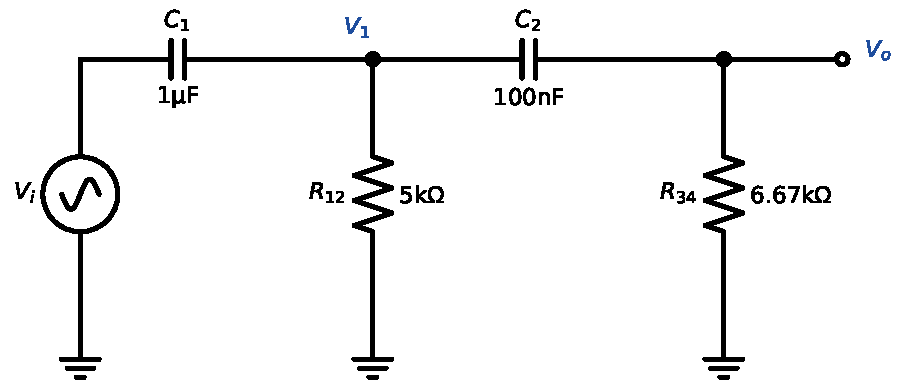
\includegraphics[width=0.95\linewidth,height=5.2cm,keepaspectratio]{p15_ac}\end{center}

\solstep{4}{Transfer function by a chain of dividers}Walk from the input to the output through the named nodes: $V_{i} \to V_{1} \to V_{o}$. The transfer function is the product of the node-to-node ratios (each one is a simple divider, tool T2, or a dependent source, tool T4):
\[
H(s) = \frac{V_o}{V_i} = \frac{V_{1}}{V_{i}}\cdot\frac{V_{o}}{V_{1}}
\]

Impedances seen \emph{looking right} from a node (everything from that node to ground, excluding what is on its left). Compute them from the far right toward the input:
\begin{align*}
Z_{1} &= R_{12} \parallel \left(\frac{1}{sC_{2}} + R_{34}\right) = \dfrac{2860\,s + 4.29\times 10^{6}}{s + 857}
\end{align*}

Now each link. {\small (Algebra tip: to simplify a fraction that contains fractions, multiply its top and bottom by every inner denominator; then divide top and bottom by the leading coefficient of the denominator so that it starts with a plain $s^n$.)}
\begin{align*}
\frac{V_{1}}{V_{i}} &= \frac{Z_{1}}{\frac{1}{sC_{1}} + Z_{1}} = \dfrac{s^{2} + 1500\,s}{s^{2} + 1850\,s + 3\times 10^{5}} \\
\frac{V_{o}}{V_{1}} &= \frac{R_{34}}{\frac{1}{sC_{2}} + R_{34}} = \dfrac{s}{s + 1500}
\end{align*}

Multiply the links and simplify (common factors cancel):\[
H(s) = \dfrac{s^{2}}{s^{2} + 1850\,s + 3\times 10^{5}}
\]

\solstep{5}{Standard (Bode-ready) form}Find the roots. Every root $s=-p$ of the denominator is a \emph{pole}, every root $s=-z$ of the numerator is a \emph{zero}; $|p|$ and $|z|$ are the corner frequencies (rad/s).
\begin{itemize}[leftmargin=*,itemsep=2pt]
\item Numerator: it has the factor $s^2$ $\Rightarrow$ 2 zeros at $s=0$.
\item Denominator: $s^{2} + 1850\,s + 3\times 10^{5}$; quadratic formula:\[
s = \frac{-1850 \pm \sqrt{(1850)^2 - 4(3\times 10^{5})}}{2} = \frac{-1850 \pm 1490}{2} \Rightarrow s = -180,\ -1670
\]

\end{itemize}

Factored form (leading coefficient in front):
\[
H(s) = 1\,\dfrac{s^{2}}{(s+180)(s+1670)}
\]

Bode-ready form: rewrite every $(s+p) = p\left(1+\frac{s}{p}\right)$ and $(s+z) = z\left(1+\frac{s}{z}\right)$, and collect all constants into $K$. Each $s$ in the numerator is paired with one of the \emph{lowest} poles as $\frac{s}{s+p}$ (that factor is $\approx 1$ above $p$). Then every factor except $K$ is $\approx 1$ inside the pass-band:
\[
H(s) = 1\,\dfrac{s}{s+2\pi\cdot 28.6}\,\dfrac{s}{s+2\pi\cdot 266},\qquad K = 1
\]

\begin{center}\renewcommand{\arraystretch}{1.35}
\begin{tabular}{cccc}
\toprule
type & $\omega_c$ (rad/s) & $f_c=\omega_c/2\pi$ & slope change \\
\midrule
pole & $180$ & 28.6 Hz & $-20$ dB/dec \\
pole & $1670$ & 266 Hz & $-20$ dB/dec \\
\bottomrule
\end{tabular}\end{center}

\solstep{6}{Magnitude Bode plot}Below every corner $|H(s)|\approx 3.33\times 10^{-6}\,s^2$, so the plot starts with a slope of $+40$\,dB/dec. Then, moving right, each pole bends the line down by 20\,dB/dec and each zero bends it up by 20\,dB/dec (tool T6):
\begin{center}\renewcommand{\arraystretch}{1.35}
\begin{tabular}{lcl}
\toprule
frequency range & slope & asymptote level \\
\midrule
$f<$ 28.6 Hz & $+40$ dB/dec & -19.4 dB at end \\
28.6 Hz -- 266 Hz & $+20$ dB/dec & -19.4 dB at start, 0 dB at end \\
$f>$ 266 Hz & $0$ dB/dec (flat) & 0 dB at start \\
\bottomrule
\end{tabular}\end{center}

The flat (pass-band) level is $20\log_{10}|K| = 20\log_{10}1 = 0$\,dB.
\begin{center}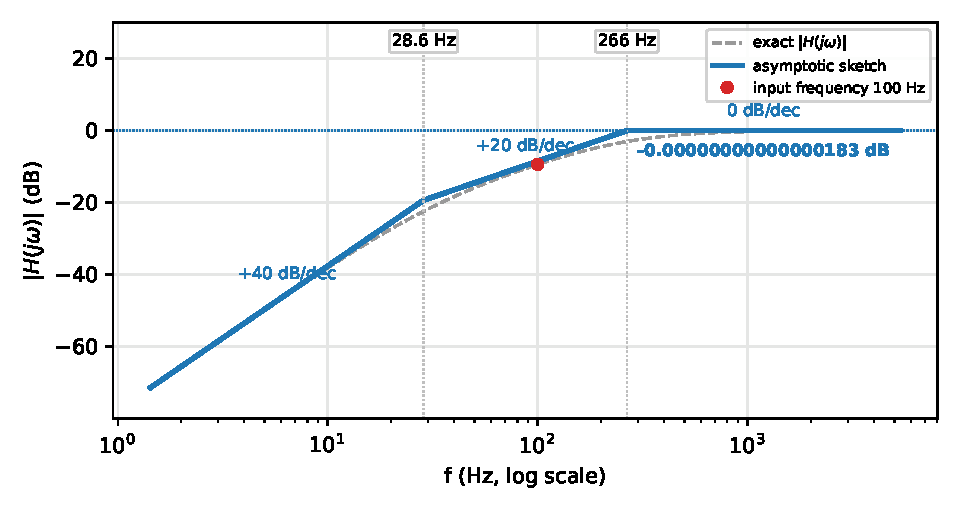
\includegraphics[width=0.78\linewidth,height=6.5cm,keepaspectratio]{p15_bode}\end{center}

{\small Blue: the straight-line sketch you are expected to draw. Dashed grey: the exact curve (about 3\,dB below the corner of an isolated pole). Red dot: the input frequency of Step 7.}
\solstep{7}{Steady-state output}The input is $V_i(t) = 0.3\sin\left(2\pi\cdot 100\,t\right)$, so $\omega_{in} = 2\pi\cdot 100 = 628$\,rad/s. Put $s=j\omega_{in}$ in each factor (tool T5): magnitudes multiply, angles add.
{\small Rules: $\left|\frac{s}{s+p}\right| = \frac{\omega}{\sqrt{\omega^2+p^2}}$, $\angle = \frac{\pi}{2}-\tan^{-1}\frac{\omega}{p}$;\quad $\left|\frac{1}{1+s/p}\right| = \frac{1}{\sqrt{1+(\omega/p)^2}}$, $\angle = -\tan^{-1}\frac{\omega}{p}$;\quad $\left|1+\frac{s}{z}\right| = \sqrt{1+(\omega/z)^2}$, $\angle = \tan^{-1}\frac{\omega}{z}$;\quad a negative $K$ adds $-\pi$.}
\begin{center}\renewcommand{\arraystretch}{1.35}
\begin{tabular}{ccc}
\toprule
factor & magnitude & angle (rad) \\
\midrule
$1$ & $1$ & $0$ \\
$\rule[-1.1em]{0pt}{2.8em}\dfrac{s}{s+2\pi\cdot 28.6}$ & $0.9615$ & $0.278$ \\
$\rule[-1.1em]{0pt}{2.8em}\dfrac{s}{s+2\pi\cdot 266}$ & $0.3521$ & $1.21$ \\
\textbf{total} & $\mathbf{0.3385}$ (product) & $\mathbf{1.49}$ (sum) \\
\bottomrule
\end{tabular}\end{center}

\begin{align*}
|H(j\omega_{in})| &= 0.339, \qquad \angle H(j\omega_{in}) = 1.49\ \mathrm{rad} \\
v_{o,ac}(t) &= 0.339\times 0.3\,\sin\left(2\pi\cdot 100\,t + 1.49\right) = 0.102\,\sin\left(2\pi\cdot 100\,t + 1.49\right)
\end{align*}

Add the DC part from Step 2 (superposition):
\[
\boxed{V_o(t) = 3.33 + 0.102\,\sin\left(2\pi\cdot 100\,t + 1.49\right)\ \mathrm{V}}
\]

\begin{ansbox}
$H(s) = 1\,\dfrac{s}{s+2\pi\cdot 28.6}\,\dfrac{s}{s+2\pi\cdot 266}$\quad (corners: 28.6 Hz, 266 Hz)\\[4pt]
$V_o(t) = 3.33 + 0.102\,\sin\left(2\pi\cdot 100\,t + 1.49\right)\ \mathrm{V}$
\end{ansbox}

\newpage
\subsection*{Solution 1B.16 \hfill Hard}
\begin{center}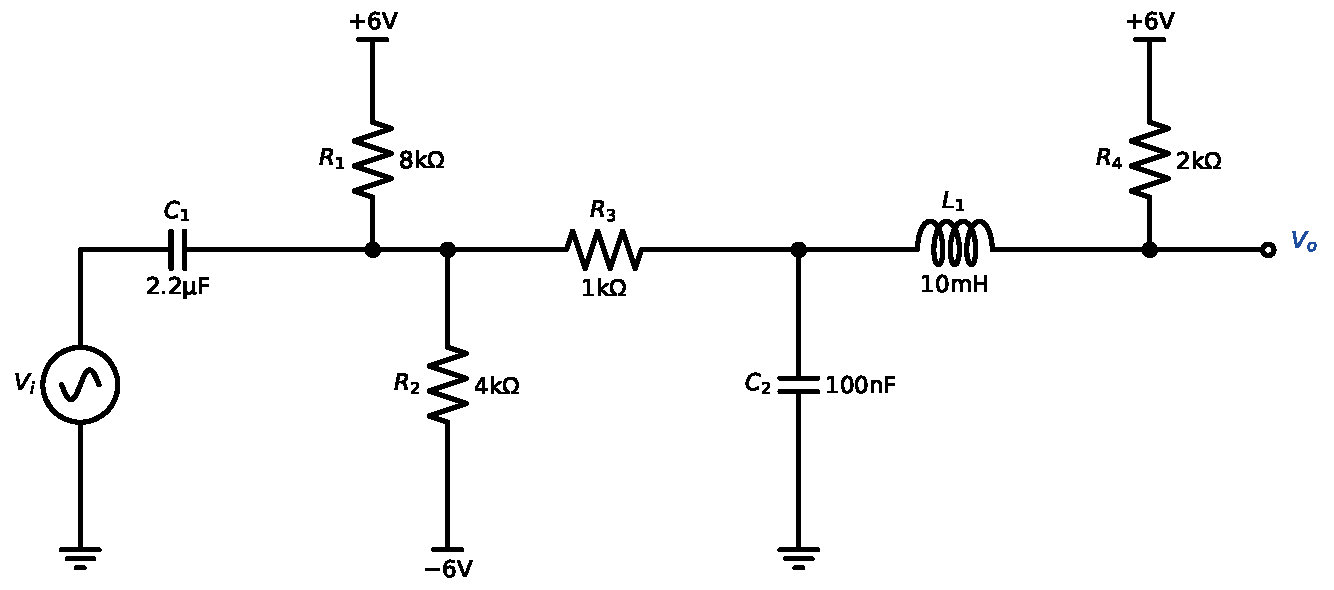
\includegraphics[width=0.8\linewidth,height=4.5cm,keepaspectratio]{p16_circuit}\end{center}
\solstep{1}{Identify the sources}Independent sources: the AC input $V_i(t)$ and the DC supplies $-6\,\mathrm{V}$, $+6\,\mathrm{V}$. Because there are both DC and AC sources, use superposition: $V_o(t) = V_{o,dc} + v_{o,ac}(t)$. Solve the DC circuit (Step 2) and the AC circuit (Steps 3--7) separately, then add.
\solstep{2}{DC circuit $\Rightarrow V_{o,dc}$}DC rules: the AC input is set to zero ($V_i=0$: a wire to ground); every capacitor is an open circuit ($C_{1}, C_{2}$); every inductor is a short circuit ($L_{1}$). Only the part of the circuit that is still connected to $V_o$ matters:
\begin{center}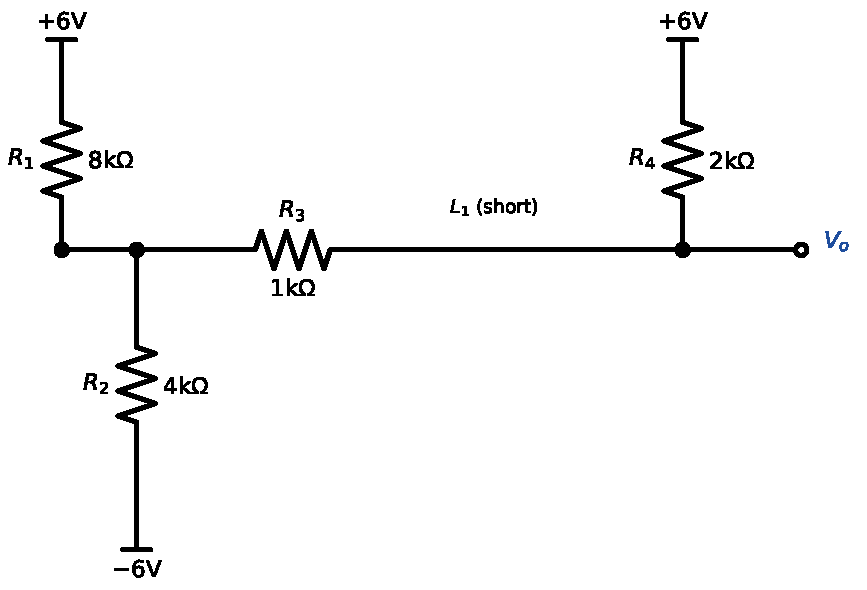
\includegraphics[width=0.55\linewidth,height=5cm,keepaspectratio]{p16_dc}\end{center}

Reduce the circuit with one tool only --- the \emph{divider between two voltages} (tool T3) --- walking toward $V_o$ and keeping a Thevenin pair $(V_{th},R_{th})$ for everything already visited.
\begin{enumerate}[leftmargin=*,itemsep=2pt]
\item Start at the input node: since $V_i=0$ it is tied to ground, i.e. it is an ideal $0\,\mathrm{V}$ source: $(V_{th},R_{th})=(0\,\mathrm{V},\,0\,\Omega)$.
\item $C_{1}$ is a capacitor $\Rightarrow$ open at DC. No DC current can cross it, so everything on its left is disconnected: start fresh after it.
\item First DC path here: $R_{1}$ to the $+6\,\mathrm{V}$ supply, so $(V_{th},R_{th}) = (6\,\mathrm{V},\ 8\,\mathrm{k}\Omega)$.
\item Add $R_{2}$ to the $-6\,\mathrm{V}$ supply. Divider between $V_a=6\,\mathrm{V}$ (through $R_a=8\,\mathrm{k}\Omega$) and $V_b=-6\,\mathrm{V}$ (through $R_b=4\,\mathrm{k}\Omega$):\[
V_{th} = V_b + (V_a-V_b)\frac{R_b}{R_a+R_b} = -6 + \left(6 - (-6)\right)\frac{4\,\mathrm{k}}{8\,\mathrm{k} + 4\,\mathrm{k}} = -2\,\mathrm{V},\qquad R_{th} = R_a\parallel R_b = 2.67\,\mathrm{k}\Omega
\]

\item Walk through $R_{3}$ ($1\,\mathrm{k}\Omega$ at DC). A series resistor just adds to $R_{th}$: $(V_{th},R_{th}) = (-2\,\mathrm{V},\ 3.67\,\mathrm{k}\Omega)$.
\item $C_{2}$ (at $V_{2}$) is a capacitor: open at DC, ignore it.
\item $L_{1}$ is a short at DC (inductor), so the pair is unchanged.
\item Finally, collect everything at the output node $V_o$.
\item Add $R_{4}$ to the $+6\,\mathrm{V}$ supply. Divider between $V_a=-2\,\mathrm{V}$ (through $R_a=3.67\,\mathrm{k}\Omega$) and $V_b=6\,\mathrm{V}$ (through $R_b=2\,\mathrm{k}\Omega$):\[
V_{th} = V_b + (V_a-V_b)\frac{R_b}{R_a+R_b} = 6 + \left(-2 - (6)\right)\frac{2\,\mathrm{k}}{3.67\,\mathrm{k} + 2\,\mathrm{k}} = 3.18\,\mathrm{V},\qquad R_{th} = R_a\parallel R_b = 1.29\,\mathrm{k}\Omega
\]

\end{enumerate}

\[
\boxed{V_{o,dc} = 3.18\,\mathrm{V}}
\]

\solstep{3}{AC circuit}Set every DC supply to zero: each supply rail becomes AC ground. Replace every capacitor by $\frac{1}{sC}$ and every inductor by $sL$.
\begin{itemize}[leftmargin=*,itemsep=2pt]
\item $R_{1}$, $R_{2}$ both go from the same node to (AC) ground, so they are in parallel: $R_{12} = R_{1} \parallel R_{2} = 8\,\mathrm{k} \parallel 4\,\mathrm{k} = 2.67\,\mathrm{k}\Omega$.
\end{itemize}

AC equivalent circuit (nodes named for the next step):
\begin{center}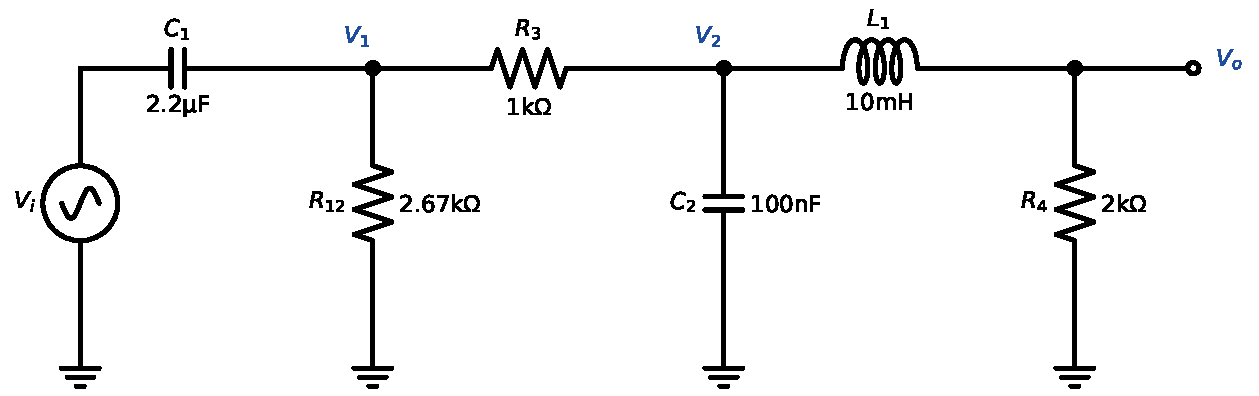
\includegraphics[width=0.95\linewidth,height=5.2cm,keepaspectratio]{p16_ac}\end{center}

\solstep{4}{Transfer function by a chain of dividers}Walk from the input to the output through the named nodes: $V_{i} \to V_{1} \to V_{2} \to V_{o}$. The transfer function is the product of the node-to-node ratios (each one is a simple divider, tool T2, or a dependent source, tool T4):
\[
H(s) = \frac{V_o}{V_i} = \frac{V_{1}}{V_{i}}\cdot\frac{V_{2}}{V_{1}}\cdot\frac{V_{o}}{V_{2}}
\]

Impedances seen \emph{looking right} from a node (everything from that node to ground, excluding what is on its left). Compute them from the far right toward the input:
\begin{align*}
Z_{2} &= \frac{1}{sC_{2}} \parallel \left(sL_{1} + R_{4}\right) = \dfrac{10^{7}\,s + 2\times 10^{12}}{s^{2} + 2\times 10^{5}\,s + 10^{9}} \\
Z_{1} &= R_{12} \parallel \left(R_{3} + Z_{2}\right) = \dfrac{727\,s^{2} + 1.53\times 10^{8}\,s + 2.18\times 10^{12}}{s^{2} + 2.03\times 10^{5}\,s + 1.55\times 10^{9}}
\end{align*}

Now each link. {\small (Algebra tip: to simplify a fraction that contains fractions, multiply its top and bottom by every inner denominator; then divide top and bottom by the leading coefficient of the denominator so that it starts with a plain $s^n$.)}
\begin{align*}
\frac{V_{1}}{V_{i}} &= \frac{Z_{1}}{\frac{1}{sC_{1}} + Z_{1}} = \dfrac{s^{3} + 2.1\times 10^{5}\,s^{2} + 3\times 10^{9}\,s}{s^{3} + 2.11\times 10^{5}\,s^{2} + 3.13\times 10^{9}\,s + 9.66\times 10^{11}} \\
\frac{V_{2}}{V_{1}} &= \frac{Z_{2}}{R_{3} + Z_{2}} = \dfrac{10000\,s + 2\times 10^{9}}{s^{2} + 2.1\times 10^{5}\,s + 3\times 10^{9}} \\
\frac{V_{o}}{V_{2}} &= \frac{R_{4}}{sL_{1} + R_{4}} = \dfrac{2\times 10^{5}}{s + 2\times 10^{5}}
\end{align*}

Multiply the links and simplify (common factors cancel):\[
H(s) = \dfrac{2\times 10^{9}\,s}{s^{3} + 2.11\times 10^{5}\,s^{2} + 3.13\times 10^{9}\,s + 9.66\times 10^{11}}
\]

\solstep{5}{Standard (Bode-ready) form}Find the roots. Every root $s=-p$ of the denominator is a \emph{pole}, every root $s=-z$ of the numerator is a \emph{zero}; $|p|$ and $|z|$ are the corner frequencies (rad/s).
\begin{itemize}[leftmargin=*,itemsep=2pt]
\item Numerator: it has the factor $s$ $\Rightarrow$ 1 zero at $s=0$.
\item Denominator: $s^{3} + 2.11\times 10^{5}\,s^{2} + 3.13\times 10^{9}\,s + 9.66\times 10^{11}$; this is degree 3: use a calculator's polynomial solver (or \texttt{numpy.roots}) $\Rightarrow s = -316,\ -15700,\ -1.95\times 10^{5}$.
\end{itemize}

Factored form (leading coefficient in front):
\[
H(s) = 2\times 10^{9}\,\dfrac{s}{(s+316)(s+15700)(s+1.95\times 10^{5})}
\]

Bode-ready form: rewrite every $(s+p) = p\left(1+\frac{s}{p}\right)$ and $(s+z) = z\left(1+\frac{s}{z}\right)$, and collect all constants into $K$. Each $s$ in the numerator is paired with one of the \emph{lowest} poles as $\frac{s}{s+p}$ (that factor is $\approx 1$ above $p$). Then every factor except $K$ is $\approx 1$ inside the pass-band:
\[
H(s) = 0.654\,\dfrac{s}{s+2\pi\cdot 50.2}\,\dfrac{1}{1+\dfrac{s}{2\pi\cdot 2.5\mathrm{k}}}\,\dfrac{1}{1+\dfrac{s}{2\pi\cdot 31\mathrm{k}}},\qquad K = 0.654
\]

\begin{center}\renewcommand{\arraystretch}{1.35}
\begin{tabular}{cccc}
\toprule
type & $\omega_c$ (rad/s) & $f_c=\omega_c/2\pi$ & slope change \\
\midrule
pole & $316$ & 50.2 Hz & $-20$ dB/dec \\
pole & $15700$ & 2.5 kHz & $-20$ dB/dec \\
pole & $1.95\times 10^{5}$ & 31 kHz & $-20$ dB/dec \\
\bottomrule
\end{tabular}\end{center}

\solstep{6}{Magnitude Bode plot}Below every corner $|H(s)|\approx 0.00207\,s$, so the plot starts with a slope of $+20$\,dB/dec. Then, moving right, each pole bends the line down by 20\,dB/dec and each zero bends it up by 20\,dB/dec (tool T6):
\begin{center}\renewcommand{\arraystretch}{1.35}
\begin{tabular}{lcl}
\toprule
frequency range & slope & asymptote level \\
\midrule
$f<$ 50.2 Hz & $+20$ dB/dec & -3.69 dB at end \\
50.2 Hz -- 2.5 kHz & $0$ dB/dec (flat) & -3.69 dB at start, -3.69 dB at end \\
2.5 kHz -- 31 kHz & $-20$ dB/dec & -3.69 dB at start, -25.5 dB at end \\
$f>$ 31 kHz & $-40$ dB/dec & -25.5 dB at start \\
\bottomrule
\end{tabular}\end{center}

The flat (pass-band) level is $20\log_{10}|K| = 20\log_{10}0.654 = -3.69$\,dB.
\begin{center}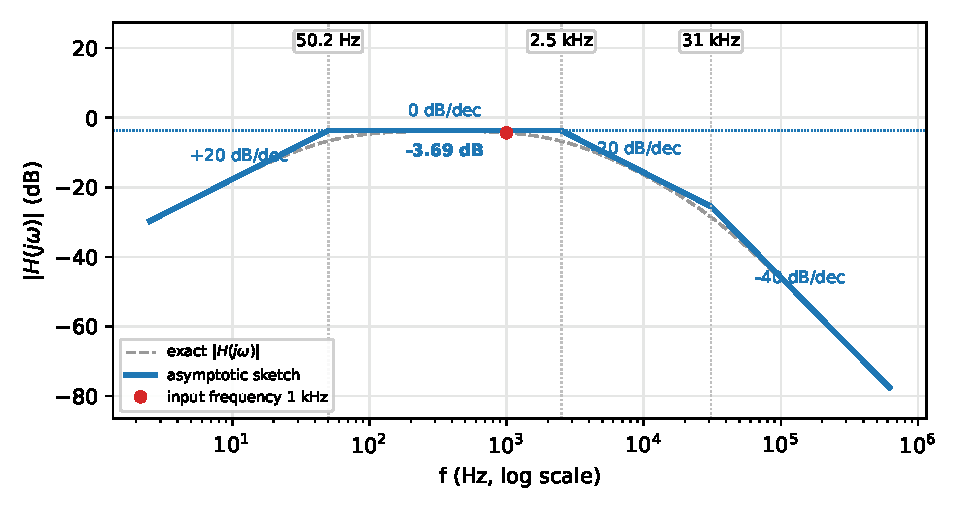
\includegraphics[width=0.78\linewidth,height=6.5cm,keepaspectratio]{p16_bode}\end{center}

{\small Blue: the straight-line sketch you are expected to draw. Dashed grey: the exact curve (about 3\,dB below the corner of an isolated pole). Red dot: the input frequency of Step 7.}
\solstep{7}{Steady-state output}The input is $V_i(t) = 1\cos\left(2\pi\cdot 1000\,t\right)$, so $\omega_{in} = 2\pi\cdot 1000 = 6280$\,rad/s. Put $s=j\omega_{in}$ in each factor (tool T5): magnitudes multiply, angles add.
{\small Rules: $\left|\frac{s}{s+p}\right| = \frac{\omega}{\sqrt{\omega^2+p^2}}$, $\angle = \frac{\pi}{2}-\tan^{-1}\frac{\omega}{p}$;\quad $\left|\frac{1}{1+s/p}\right| = \frac{1}{\sqrt{1+(\omega/p)^2}}$, $\angle = -\tan^{-1}\frac{\omega}{p}$;\quad $\left|1+\frac{s}{z}\right| = \sqrt{1+(\omega/z)^2}$, $\angle = \tan^{-1}\frac{\omega}{z}$;\quad a negative $K$ adds $-\pi$.}
\begin{center}\renewcommand{\arraystretch}{1.35}
\begin{tabular}{ccc}
\toprule
factor & magnitude & angle (rad) \\
\midrule
$0.654$ & $0.6535$ & $0$ \\
$\rule[-1.1em]{0pt}{2.8em}\dfrac{s}{s+2\pi\cdot 50.2}$ & $0.9987$ & $0.0502$ \\
$\rule[-1.7em]{0pt}{4em}\dfrac{1}{1+\dfrac{s}{2\pi\cdot 2.5\mathrm{k}}}$ & $0.9286$ & $-0.38$ \\
$\rule[-1.7em]{0pt}{4em}\dfrac{1}{1+\dfrac{s}{2\pi\cdot 31\mathrm{k}}}$ & $0.9995$ & $-0.0323$ \\
\textbf{total} & $\mathbf{0.6058}$ (product) & $\mathbf{-0.362}$ (sum) \\
\bottomrule
\end{tabular}\end{center}

\begin{align*}
|H(j\omega_{in})| &= 0.606, \qquad \angle H(j\omega_{in}) = -0.362\ \mathrm{rad} \\
v_{o,ac}(t) &= 0.606\times 1\,\cos\left(2\pi\cdot 1000\,t - 0.362\right) = 0.606\,\cos\left(2\pi\cdot 1000\,t - 0.362\right)
\end{align*}

Add the DC part from Step 2 (superposition):
\[
\boxed{V_o(t) = 3.18 + 0.606\,\cos\left(2\pi\cdot 1000\,t - 0.362\right)\ \mathrm{V}}
\]

\begin{ansbox}
$H(s) = 0.654\,\dfrac{s}{s+2\pi\cdot 50.2}\,\dfrac{1}{1+\dfrac{s}{2\pi\cdot 2.5\mathrm{k}}}\,\dfrac{1}{1+\dfrac{s}{2\pi\cdot 31\mathrm{k}}}$\quad (corners: 50.2 Hz, 2.5 kHz, 31 kHz)\\[4pt]
$V_o(t) = 3.18 + 0.606\,\cos\left(2\pi\cdot 1000\,t - 0.362\right)\ \mathrm{V}$
\end{ansbox}

\newpage
\subsection*{Solution 1B.17 \hfill Hard}
\begin{center}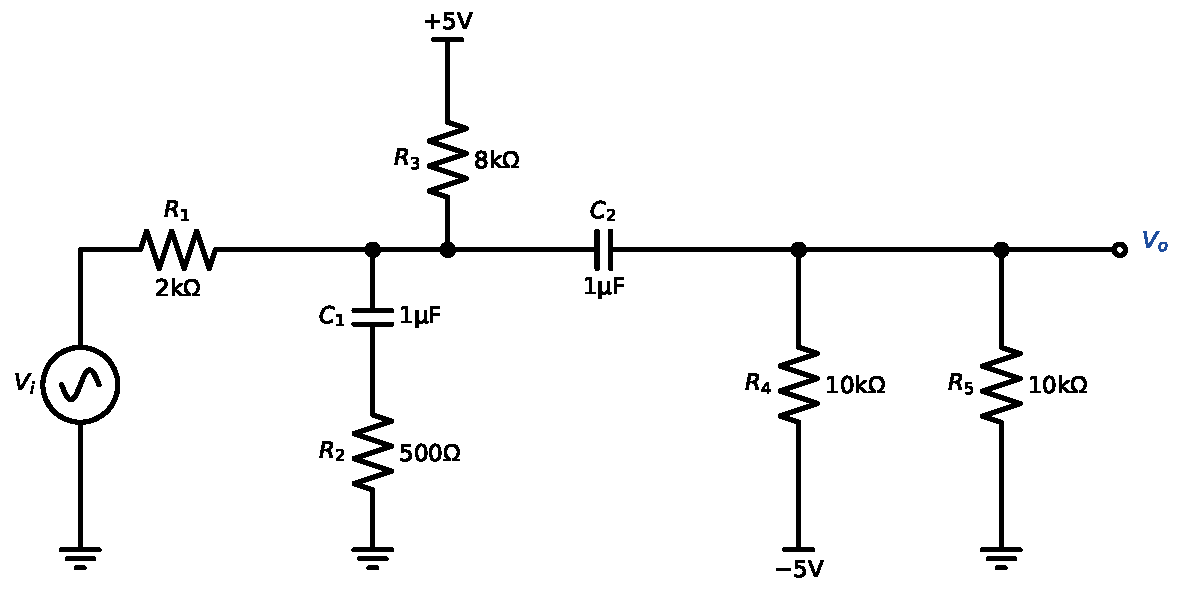
\includegraphics[width=0.8\linewidth,height=4.5cm,keepaspectratio]{p17_circuit}\end{center}
\solstep{1}{Identify the sources}Independent sources: the AC input $V_i(t)$ and the DC supplies $-5\,\mathrm{V}$, $+5\,\mathrm{V}$. Because there are both DC and AC sources, use superposition: $V_o(t) = V_{o,dc} + v_{o,ac}(t)$. Solve the DC circuit (Step 2) and the AC circuit (Steps 3--7) separately, then add.
\solstep{2}{DC circuit $\Rightarrow V_{o,dc}$}DC rules: the AC input is set to zero ($V_i=0$: a wire to ground); every capacitor is an open circuit ($C_{1}, C_{2}$). Only the part of the circuit that is still connected to $V_o$ matters:
\begin{center}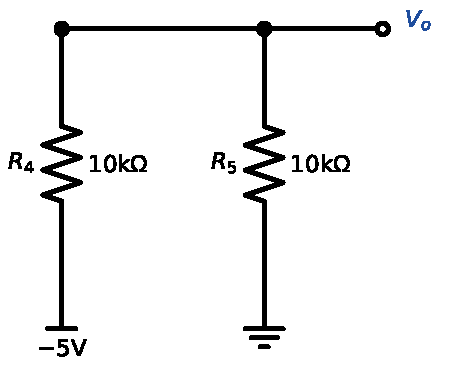
\includegraphics[width=0.55\linewidth,height=5cm,keepaspectratio]{p17_dc}\end{center}

Reduce the circuit with one tool only --- the \emph{divider between two voltages} (tool T3) --- walking toward $V_o$ and keeping a Thevenin pair $(V_{th},R_{th})$ for everything already visited.
\begin{enumerate}[leftmargin=*,itemsep=2pt]
\item Start at the input node: since $V_i=0$ it is tied to ground, i.e. it is an ideal $0\,\mathrm{V}$ source: $(V_{th},R_{th})=(0\,\mathrm{V},\,0\,\Omega)$.
\item Walk through $R_{1}$ ($2\,\mathrm{k}\Omega$ at DC). A series resistor just adds to $R_{th}$: $(V_{th},R_{th}) = (0\,\mathrm{V},\ 2\,\mathrm{k}\Omega)$.
\item $C_{1} + R_{2}$ (at $V_{1}$) contains a capacitor: open at DC, ignore it.
\item Add $R_{3}$ to the $+5\,\mathrm{V}$ supply. Divider between $V_a=0\,\mathrm{V}$ (through $R_a=2\,\mathrm{k}\Omega$) and $V_b=5\,\mathrm{V}$ (through $R_b=8\,\mathrm{k}\Omega$):\[
V_{th} = V_b + (V_a-V_b)\frac{R_b}{R_a+R_b} = 5 + \left(0 - (5)\right)\frac{8\,\mathrm{k}}{2\,\mathrm{k} + 8\,\mathrm{k}} = 1\,\mathrm{V},\qquad R_{th} = R_a\parallel R_b = 1.6\,\mathrm{k}\Omega
\]

\item $C_{2}$ is a capacitor $\Rightarrow$ open at DC. No DC current can cross it, so everything on its left is disconnected: start fresh after it.
\item Finally, collect everything at the output node $V_o$.
\item First DC path here: $R_{4}$ to the $-5\,\mathrm{V}$ supply, so $(V_{th},R_{th}) = (-5\,\mathrm{V},\ 10\,\mathrm{k}\Omega)$.
\item Add $R_{5}$ to ground. Divider between $V_a=-5\,\mathrm{V}$ (through $R_a=10\,\mathrm{k}\Omega$) and $V_b=0\,\mathrm{V}$ (through $R_b=10\,\mathrm{k}\Omega$):\[
V_{th} = V_b + (V_a-V_b)\frac{R_b}{R_a+R_b} = 0 + \left(-5 - (0)\right)\frac{10\,\mathrm{k}}{10\,\mathrm{k} + 10\,\mathrm{k}} = -2.5\,\mathrm{V},\qquad R_{th} = R_a\parallel R_b = 5\,\mathrm{k}\Omega
\]

\end{enumerate}

\[
\boxed{V_{o,dc} = -2.5\,\mathrm{V}}
\]

\solstep{3}{AC circuit}Set every DC supply to zero: each supply rail becomes AC ground. Replace every capacitor by $\frac{1}{sC}$ and every inductor by $sL$.
\begin{itemize}[leftmargin=*,itemsep=2pt]
\item $R_{4}$, $R_{5}$ both go from the same node to (AC) ground, so they are in parallel: $R_{45} = R_{4} \parallel R_{5} = 10\,\mathrm{k} \parallel 10\,\mathrm{k} = 5\,\mathrm{k}\Omega$.
\end{itemize}

AC equivalent circuit (nodes named for the next step):
\begin{center}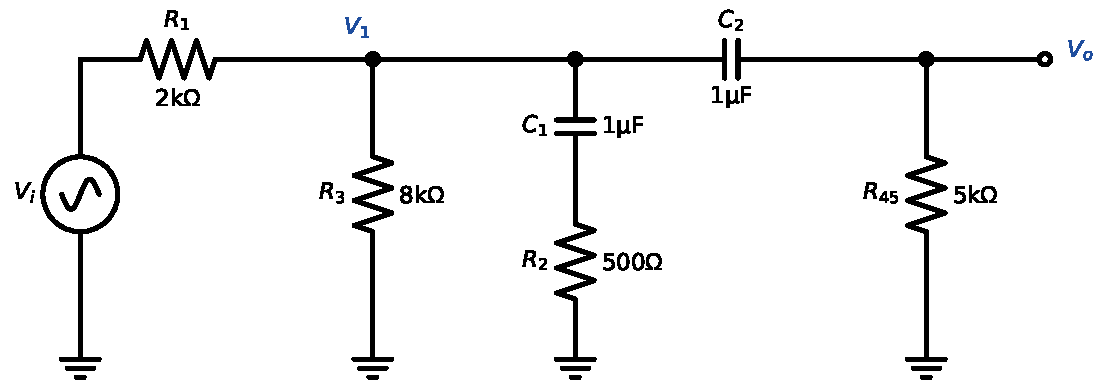
\includegraphics[width=0.95\linewidth,height=5.2cm,keepaspectratio]{p17_ac}\end{center}

\solstep{4}{Transfer function by a chain of dividers}Walk from the input to the output through the named nodes: $V_{i} \to V_{1} \to V_{o}$. The transfer function is the product of the node-to-node ratios (each one is a simple divider, tool T2, or a dependent source, tool T4):
\[
H(s) = \frac{V_o}{V_i} = \frac{V_{1}}{V_{i}}\cdot\frac{V_{o}}{V_{1}}
\]

Impedances seen \emph{looking right} from a node (everything from that node to ground, excluding what is on its left). Compute them from the far right toward the input:
\begin{align*}
Z_{1} &= R_{3} \parallel \left(\frac{1}{sC_{1}} + R_{2}\right) \parallel \left(\frac{1}{sC_{2}} + R_{45}\right) = \dfrac{430\,s^{2} + 9.46\times 10^{5}\,s + 1.72\times 10^{8}}{s^{2} + 462\,s + 21500}
\end{align*}

Now each link. {\small (Algebra tip: to simplify a fraction that contains fractions, multiply its top and bottom by every inner denominator; then divide top and bottom by the leading coefficient of the denominator so that it starts with a plain $s^n$.)}
\begin{align*}
\frac{V_{1}}{V_{i}} &= \frac{Z_{1}}{R_{1} + Z_{1}} = \dfrac{0.177\,s^{2} + 389\,s + 70800}{s^{2} + 770\,s + 88500} \\
\frac{V_{o}}{V_{1}} &= \frac{R_{45}}{\frac{1}{sC_{2}} + R_{45}} = \dfrac{s}{s + 200}
\end{align*}

Multiply the links and simplify (common factors cancel):\[
H(s) = \dfrac{0.177\,s^{2} + 354\,s}{s^{2} + 770\,s + 88500}
\]

\solstep{5}{Standard (Bode-ready) form}Find the roots. Every root $s=-p$ of the denominator is a \emph{pole}, every root $s=-z$ of the numerator is a \emph{zero}; $|p|$ and $|z|$ are the corner frequencies (rad/s).
\begin{itemize}[leftmargin=*,itemsep=2pt]
\item Numerator: it has the factor $s$ $\Rightarrow$ 1 zero at $s=0$.
\item Numerator (after taking out the $s$ factor): $0.177\,s + 354$; divide by the leading coefficient $0.177$ (this does not move the roots): $s + 2000$; $s + 2000 = 0 \Rightarrow s = -2000$.
\item Denominator: $s^{2} + 770\,s + 88500$; quadratic formula:\[
s = \frac{-770 \pm \sqrt{(770)^2 - 4(88500)}}{2} = \frac{-770 \pm 489}{2} \Rightarrow s = -141,\ -629
\]

\end{itemize}

Factored form (leading coefficient in front):
\[
H(s) = 0.177\,\dfrac{s(s+2000)}{(s+141)(s+629)}
\]

Bode-ready form: rewrite every $(s+p) = p\left(1+\frac{s}{p}\right)$ and $(s+z) = z\left(1+\frac{s}{z}\right)$, and collect all constants into $K$. Each $s$ in the numerator is paired with one of the \emph{lowest} poles as $\frac{s}{s+p}$ (that factor is $\approx 1$ above $p$). Then every factor except $K$ is $\approx 1$ inside the pass-band:
\[
H(s) = 0.563\,\dfrac{s}{s+2\pi\cdot 22.4}\,\dfrac{1}{1+\dfrac{s}{2\pi\cdot 100}}\,\left(1+\dfrac{s}{2\pi\cdot 318}\right),\qquad K = 0.563
\]

\begin{center}\renewcommand{\arraystretch}{1.35}
\begin{tabular}{cccc}
\toprule
type & $\omega_c$ (rad/s) & $f_c=\omega_c/2\pi$ & slope change \\
\midrule
pole & $141$ & 22.4 Hz & $-20$ dB/dec \\
pole & $629$ & 100 Hz & $-20$ dB/dec \\
zero & $2000$ & 318 Hz & $+20$ dB/dec \\
\bottomrule
\end{tabular}\end{center}

\solstep{6}{Magnitude Bode plot}Below every corner $|H(s)|\approx 0.004\,s$, so the plot starts with a slope of $+20$\,dB/dec. Then, moving right, each pole bends the line down by 20\,dB/dec and each zero bends it up by 20\,dB/dec (tool T6):
\begin{center}\renewcommand{\arraystretch}{1.35}
\begin{tabular}{lcl}
\toprule
frequency range & slope & asymptote level \\
\midrule
$f<$ 22.4 Hz & $+20$ dB/dec & -5 dB at end \\
22.4 Hz -- 100 Hz & $0$ dB/dec (flat) & -5 dB at start, -5 dB at end \\
100 Hz -- 318 Hz & $-20$ dB/dec & -5 dB at start, -15 dB at end \\
$f>$ 318 Hz & $0$ dB/dec (flat) & -15 dB at start \\
\bottomrule
\end{tabular}\end{center}

\begin{center}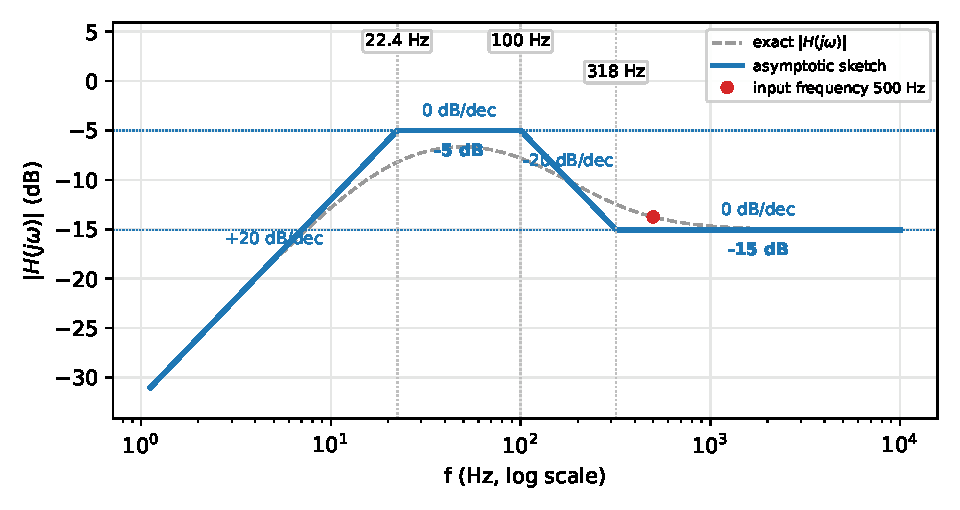
\includegraphics[width=0.78\linewidth,height=6.5cm,keepaspectratio]{p17_bode}\end{center}

{\small Blue: the straight-line sketch you are expected to draw. Dashed grey: the exact curve (about 3\,dB below the corner of an isolated pole). Red dot: the input frequency of Step 7.}
\solstep{7}{Steady-state output}The input is $V_i(t) = 1\cos\left(2\pi\cdot 500\,t-\frac{\pi}{3}\right)$, so $\omega_{in} = 2\pi\cdot 500 = 3140$\,rad/s. Put $s=j\omega_{in}$ in each factor (tool T5): magnitudes multiply, angles add.
{\small Rules: $\left|\frac{s}{s+p}\right| = \frac{\omega}{\sqrt{\omega^2+p^2}}$, $\angle = \frac{\pi}{2}-\tan^{-1}\frac{\omega}{p}$;\quad $\left|\frac{1}{1+s/p}\right| = \frac{1}{\sqrt{1+(\omega/p)^2}}$, $\angle = -\tan^{-1}\frac{\omega}{p}$;\quad $\left|1+\frac{s}{z}\right| = \sqrt{1+(\omega/z)^2}$, $\angle = \tan^{-1}\frac{\omega}{z}$;\quad a negative $K$ adds $-\pi$.}
\begin{center}\renewcommand{\arraystretch}{1.35}
\begin{tabular}{ccc}
\toprule
factor & magnitude & angle (rad) \\
\midrule
$0.563$ & $0.5625$ & $0$ \\
$\rule[-1.1em]{0pt}{2.8em}\dfrac{s}{s+2\pi\cdot 22.4}$ & $0.999$ & $0.0447$ \\
$\rule[-1.7em]{0pt}{4em}\dfrac{1}{1+\dfrac{s}{2\pi\cdot 100}}$ & $0.1964$ & $-1.37$ \\
$\rule[-1.1em]{0pt}{2.8em}\left(1+\dfrac{s}{2\pi\cdot 318}\right)$ & $1.862$ & $1$ \\
\textbf{total} & $\mathbf{0.2055}$ (product) & $\mathbf{-0.324}$ (sum) \\
\bottomrule
\end{tabular}\end{center}

\begin{align*}
|H(j\omega_{in})| &= 0.206, \qquad \angle H(j\omega_{in}) = -0.324\ \mathrm{rad} \\
v_{o,ac}(t) &= 0.206\times 1\,\cos\left(2\pi\cdot 500\,t - 1.37\right) = 0.206\,\cos\left(2\pi\cdot 500\,t - 1.37\right)
\end{align*}

(phase: $\theta + \angle H = -\frac{\pi}{3} + (-0.324) = -1.37$\,rad.)
Add the DC part from Step 2 (superposition):
\[
\boxed{V_o(t) = -2.5 + 0.206\,\cos\left(2\pi\cdot 500\,t - 1.37\right)\ \mathrm{V}}
\]

\begin{ansbox}
$H(s) = 0.563\,\dfrac{s}{s+2\pi\cdot 22.4}\,\dfrac{1}{1+\dfrac{s}{2\pi\cdot 100}}\,\left(1+\dfrac{s}{2\pi\cdot 318}\right)$\quad (corners: 22.4 Hz, 100 Hz, 318 Hz)\\[4pt]
$V_o(t) = -2.5 + 0.206\,\cos\left(2\pi\cdot 500\,t - 1.37\right)\ \mathrm{V}$
\end{ansbox}

\newpage
\subsection*{Solution 1B.18 \hfill Hard}
\begin{center}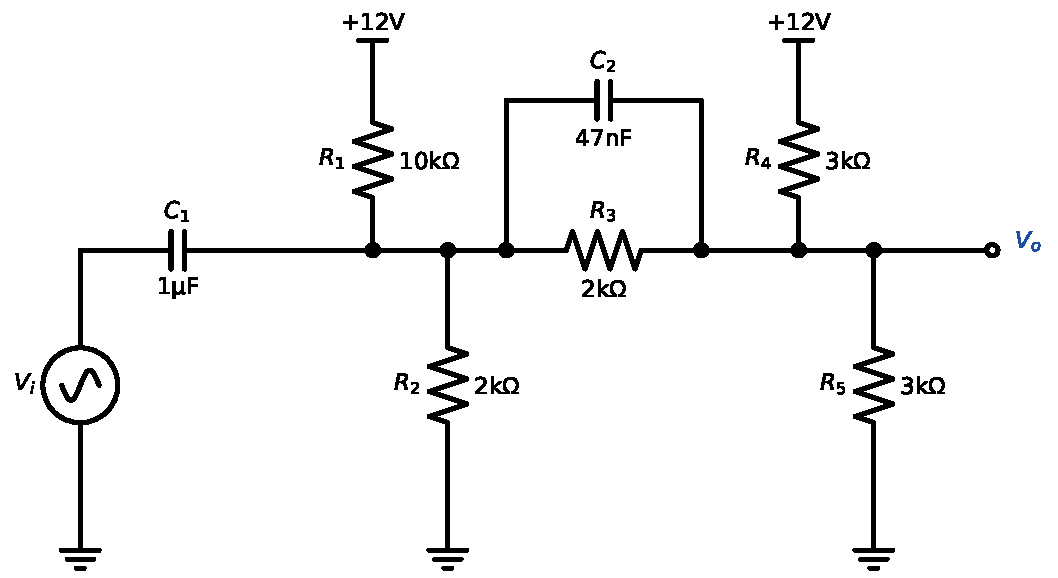
\includegraphics[width=0.8\linewidth,height=4.5cm,keepaspectratio]{p18_circuit}\end{center}
\solstep{1}{Identify the sources}Independent sources: the AC input $V_i(t)$ and the DC supplies $+12\,\mathrm{V}$. Because there are both DC and AC sources, use superposition: $V_o(t) = V_{o,dc} + v_{o,ac}(t)$. Solve the DC circuit (Step 2) and the AC circuit (Steps 3--7) separately, then add.
\solstep{2}{DC circuit $\Rightarrow V_{o,dc}$}DC rules: the AC input is set to zero ($V_i=0$: a wire to ground); every capacitor is an open circuit ($C_{1}, C_{2}$). Only the part of the circuit that is still connected to $V_o$ matters:
\begin{center}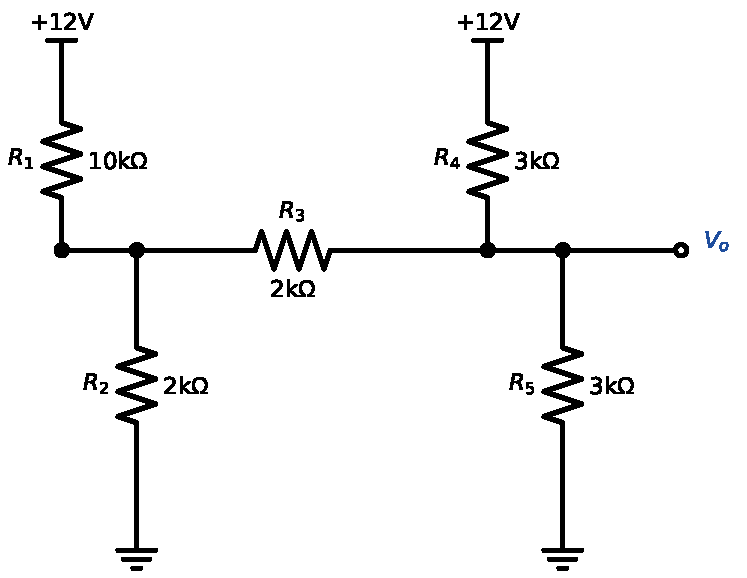
\includegraphics[width=0.55\linewidth,height=5cm,keepaspectratio]{p18_dc}\end{center}

Reduce the circuit with one tool only --- the \emph{divider between two voltages} (tool T3) --- walking toward $V_o$ and keeping a Thevenin pair $(V_{th},R_{th})$ for everything already visited.
\begin{enumerate}[leftmargin=*,itemsep=2pt]
\item Start at the input node: since $V_i=0$ it is tied to ground, i.e. it is an ideal $0\,\mathrm{V}$ source: $(V_{th},R_{th})=(0\,\mathrm{V},\,0\,\Omega)$.
\item $C_{1}$ is a capacitor $\Rightarrow$ open at DC. No DC current can cross it, so everything on its left is disconnected: start fresh after it.
\item First DC path here: $R_{1}$ to the $+12\,\mathrm{V}$ supply, so $(V_{th},R_{th}) = (12\,\mathrm{V},\ 10\,\mathrm{k}\Omega)$.
\item Add $R_{2}$ to ground. Divider between $V_a=12\,\mathrm{V}$ (through $R_a=10\,\mathrm{k}\Omega$) and $V_b=0\,\mathrm{V}$ (through $R_b=2\,\mathrm{k}\Omega$):\[
V_{th} = V_b + (V_a-V_b)\frac{R_b}{R_a+R_b} = 0 + \left(12 - (0)\right)\frac{2\,\mathrm{k}}{10\,\mathrm{k} + 2\,\mathrm{k}} = 2\,\mathrm{V},\qquad R_{th} = R_a\parallel R_b = 1.67\,\mathrm{k}\Omega
\]

\item Walk through $R_{3} \parallel C_{2}$ ($2\,\mathrm{k}\Omega$ at DC). A series resistor just adds to $R_{th}$: $(V_{th},R_{th}) = (2\,\mathrm{V},\ 3.67\,\mathrm{k}\Omega)$.
\item Finally, collect everything at the output node $V_o$.
\item Add $R_{4}$ to the $+12\,\mathrm{V}$ supply. Divider between $V_a=2\,\mathrm{V}$ (through $R_a=3.67\,\mathrm{k}\Omega$) and $V_b=12\,\mathrm{V}$ (through $R_b=3\,\mathrm{k}\Omega$):\[
V_{th} = V_b + (V_a-V_b)\frac{R_b}{R_a+R_b} = 12 + \left(2 - (12)\right)\frac{3\,\mathrm{k}}{3.67\,\mathrm{k} + 3\,\mathrm{k}} = 7.5\,\mathrm{V},\qquad R_{th} = R_a\parallel R_b = 1.65\,\mathrm{k}\Omega
\]

\item Add $R_{5}$ to ground. Divider between $V_a=7.5\,\mathrm{V}$ (through $R_a=1.65\,\mathrm{k}\Omega$) and $V_b=0\,\mathrm{V}$ (through $R_b=3\,\mathrm{k}\Omega$):\[
V_{th} = V_b + (V_a-V_b)\frac{R_b}{R_a+R_b} = 0 + \left(7.5 - (0)\right)\frac{3\,\mathrm{k}}{1.65\,\mathrm{k} + 3\,\mathrm{k}} = 4.84\,\mathrm{V},\qquad R_{th} = R_a\parallel R_b = 1.06\,\mathrm{k}\Omega
\]

\end{enumerate}

\[
\boxed{V_{o,dc} = 4.84\,\mathrm{V}}
\]

\solstep{3}{AC circuit}Set every DC supply to zero: each supply rail becomes AC ground. Replace every capacitor by $\frac{1}{sC}$ and every inductor by $sL$.
\begin{itemize}[leftmargin=*,itemsep=2pt]
\item $R_{1}$, $R_{2}$ both go from the same node to (AC) ground, so they are in parallel: $R_{12} = R_{1} \parallel R_{2} = 10\,\mathrm{k} \parallel 2\,\mathrm{k} = 1.67\,\mathrm{k}\Omega$.
\item $R_{4}$, $R_{5}$ both go from the same node to (AC) ground, so they are in parallel: $R_{45} = R_{4} \parallel R_{5} = 3\,\mathrm{k} \parallel 3\,\mathrm{k} = 1.5\,\mathrm{k}\Omega$.
\end{itemize}

AC equivalent circuit (nodes named for the next step):
\begin{center}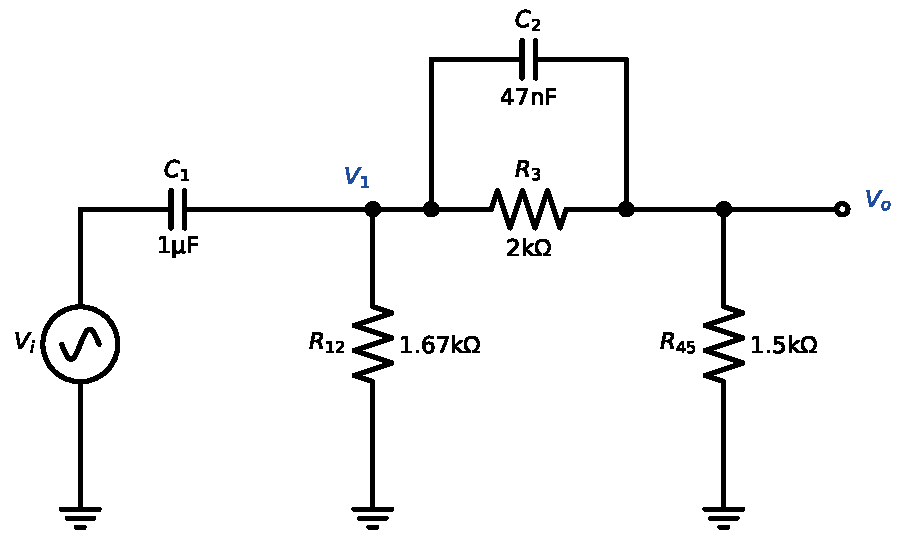
\includegraphics[width=0.95\linewidth,height=5.2cm,keepaspectratio]{p18_ac}\end{center}

\solstep{4}{Transfer function by a chain of dividers}Walk from the input to the output through the named nodes: $V_{i} \to V_{1} \to V_{o}$. The transfer function is the product of the node-to-node ratios (each one is a simple divider, tool T2, or a dependent source, tool T4):
\[
H(s) = \frac{V_o}{V_i} = \frac{V_{1}}{V_{i}}\cdot\frac{V_{o}}{V_{1}}
\]

Impedances seen \emph{looking right} from a node (everything from that node to ground, excluding what is on its left). Compute them from the far right toward the input:
\begin{align*}
Z_{1} &= R_{12} \parallel \left(\left(R_{3} \parallel \frac{1}{sC_{2}}\right) + R_{45}\right) = \dfrac{789\,s + 1.96\times 10^{7}}{s + 17400}
\end{align*}

Now each link. {\small (Algebra tip: to simplify a fraction that contains fractions, multiply its top and bottom by every inner denominator; then divide top and bottom by the leading coefficient of the denominator so that it starts with a plain $s^n$.)}
\begin{align*}
\frac{V_{1}}{V_{i}} &= \frac{Z_{1}}{\frac{1}{sC_{1}} + Z_{1}} = \dfrac{s^{2} + 24800\,s}{s^{2} + 26100\,s + 2.2\times 10^{7}} \\
\frac{V_{o}}{V_{1}} &= \frac{R_{45}}{R_{3} \parallel \frac{1}{sC_{2}} + R_{45}} = \dfrac{s + 10600}{s + 24800}
\end{align*}

Multiply the links and simplify (common factors cancel):\[
H(s) = \dfrac{s^{2} + 10600\,s}{s^{2} + 26100\,s + 2.2\times 10^{7}}
\]

\solstep{5}{Standard (Bode-ready) form}Find the roots. Every root $s=-p$ of the denominator is a \emph{pole}, every root $s=-z$ of the numerator is a \emph{zero}; $|p|$ and $|z|$ are the corner frequencies (rad/s).
\begin{itemize}[leftmargin=*,itemsep=2pt]
\item Numerator: it has the factor $s$ $\Rightarrow$ 1 zero at $s=0$.
\item Numerator (after taking out the $s$ factor): $s + 10600$; $s + 10600 = 0 \Rightarrow s = -10600$.
\item Denominator: $s^{2} + 26100\,s + 2.2\times 10^{7}$; quadratic formula:\[
s = \frac{-26100 \pm \sqrt{(26100)^2 - 4(2.2\times 10^{7})}}{2} = \frac{-26100 \pm 24300}{2} \Rightarrow s = -872,\ -25200
\]

\end{itemize}

Factored form (leading coefficient in front):
\[
H(s) = 1\,\dfrac{s(s+10600)}{(s+872)(s+25200)}
\]

Bode-ready form: rewrite every $(s+p) = p\left(1+\frac{s}{p}\right)$ and $(s+z) = z\left(1+\frac{s}{z}\right)$, and collect all constants into $K$. Each $s$ in the numerator is paired with one of the \emph{lowest} poles as $\frac{s}{s+p}$ (that factor is $\approx 1$ above $p$). Then every factor except $K$ is $\approx 1$ inside the pass-band:
\[
H(s) = 0.422\,\dfrac{s}{s+2\pi\cdot 139}\,\left(1+\dfrac{s}{2\pi\cdot 1.69\mathrm{k}}\right)\,\dfrac{1}{1+\dfrac{s}{2\pi\cdot 4.01\mathrm{k}}},\qquad K = 0.422
\]

\begin{center}\renewcommand{\arraystretch}{1.35}
\begin{tabular}{cccc}
\toprule
type & $\omega_c$ (rad/s) & $f_c=\omega_c/2\pi$ & slope change \\
\midrule
pole & $872$ & 139 Hz & $-20$ dB/dec \\
zero & $10600$ & 1.69 kHz & $+20$ dB/dec \\
pole & $25200$ & 4.01 kHz & $-20$ dB/dec \\
\bottomrule
\end{tabular}\end{center}

\solstep{6}{Magnitude Bode plot}Below every corner $|H(s)|\approx 4.84\times 10^{-4}\,s$, so the plot starts with a slope of $+20$\,dB/dec. Then, moving right, each pole bends the line down by 20\,dB/dec and each zero bends it up by 20\,dB/dec (tool T6):
\begin{center}\renewcommand{\arraystretch}{1.35}
\begin{tabular}{lcl}
\toprule
frequency range & slope & asymptote level \\
\midrule
$f<$ 139 Hz & $+20$ dB/dec & -7.5 dB at end \\
139 Hz -- 1.69 kHz & $0$ dB/dec (flat) & -7.5 dB at start, -7.5 dB at end \\
1.69 kHz -- 4.01 kHz & $+20$ dB/dec & -7.5 dB at start, 0 dB at end \\
$f>$ 4.01 kHz & $0$ dB/dec (flat) & 0 dB at start \\
\bottomrule
\end{tabular}\end{center}

\begin{center}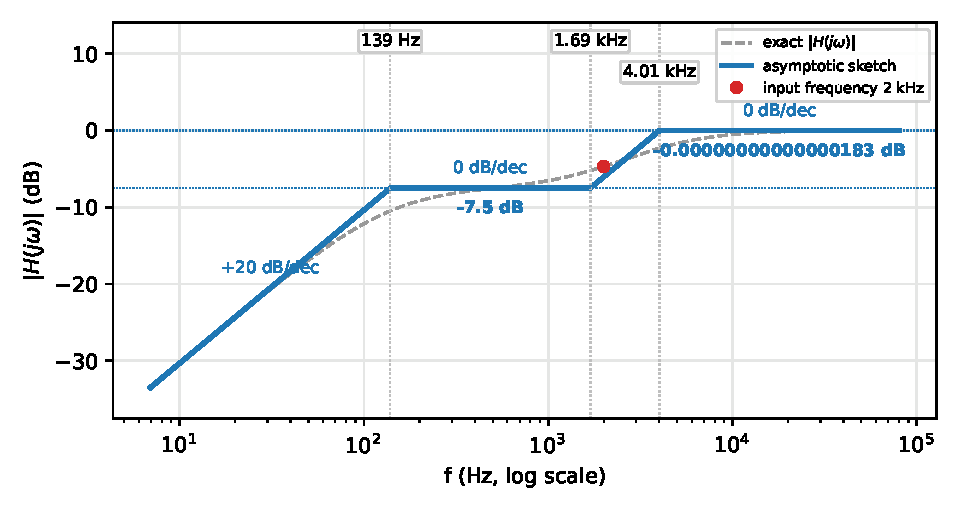
\includegraphics[width=0.78\linewidth,height=6.5cm,keepaspectratio]{p18_bode}\end{center}

{\small Blue: the straight-line sketch you are expected to draw. Dashed grey: the exact curve (about 3\,dB below the corner of an isolated pole). Red dot: the input frequency of Step 7.}
\solstep{7}{Steady-state output}The input is $V_i(t) = 0.5\sin\left(2\pi\cdot 2000\,t+\frac{\pi}{6}\right)$, so $\omega_{in} = 2\pi\cdot 2000 = 12600$\,rad/s. Put $s=j\omega_{in}$ in each factor (tool T5): magnitudes multiply, angles add.
{\small Rules: $\left|\frac{s}{s+p}\right| = \frac{\omega}{\sqrt{\omega^2+p^2}}$, $\angle = \frac{\pi}{2}-\tan^{-1}\frac{\omega}{p}$;\quad $\left|\frac{1}{1+s/p}\right| = \frac{1}{\sqrt{1+(\omega/p)^2}}$, $\angle = -\tan^{-1}\frac{\omega}{p}$;\quad $\left|1+\frac{s}{z}\right| = \sqrt{1+(\omega/z)^2}$, $\angle = \tan^{-1}\frac{\omega}{z}$;\quad a negative $K$ adds $-\pi$.}
\begin{center}\renewcommand{\arraystretch}{1.35}
\begin{tabular}{ccc}
\toprule
factor & magnitude & angle (rad) \\
\midrule
$0.422$ & $0.4219$ & $0$ \\
$\rule[-1.1em]{0pt}{2.8em}\dfrac{s}{s+2\pi\cdot 139}$ & $0.9976$ & $0.0693$ \\
$\rule[-1.1em]{0pt}{2.8em}\left(1+\dfrac{s}{2\pi\cdot 1.69\mathrm{k}}\right)$ & $1.548$ & $0.868$ \\
$\rule[-1.7em]{0pt}{4em}\dfrac{1}{1+\dfrac{s}{2\pi\cdot 4.01\mathrm{k}}}$ & $0.895$ & $-0.462$ \\
\textbf{total} & $\mathbf{0.583}$ (product) & $\mathbf{0.475}$ (sum) \\
\bottomrule
\end{tabular}\end{center}

\begin{align*}
|H(j\omega_{in})| &= 0.583, \qquad \angle H(j\omega_{in}) = 0.475\ \mathrm{rad} \\
v_{o,ac}(t) &= 0.583\times 0.5\,\sin\left(2\pi\cdot 2000\,t + 0.999\right) = 0.291\,\sin\left(2\pi\cdot 2000\,t + 0.999\right)
\end{align*}

(phase: $\theta + \angle H = \frac{\pi}{6} + (0.475) = 0.999$\,rad.)
Add the DC part from Step 2 (superposition):
\[
\boxed{V_o(t) = 4.84 + 0.291\,\sin\left(2\pi\cdot 2000\,t + 0.999\right)\ \mathrm{V}}
\]

\begin{ansbox}
$H(s) = 0.422\,\dfrac{s}{s+2\pi\cdot 139}\,\left(1+\dfrac{s}{2\pi\cdot 1.69\mathrm{k}}\right)\,\dfrac{1}{1+\dfrac{s}{2\pi\cdot 4.01\mathrm{k}}}$\quad (corners: 139 Hz, 1.69 kHz, 4.01 kHz)\\[4pt]
$V_o(t) = 4.84 + 0.291\,\sin\left(2\pi\cdot 2000\,t + 0.999\right)\ \mathrm{V}$
\end{ansbox}

\end{document}
